\documentclass[a4paper,11pt,twoside]{report}
\usepackage[left=3cm,right=2.5cm,top=2.5cm,bottom=2.5cm]{geometry}
\usepackage{graphicx}
\graphicspath{{LateX images/}}
\usepackage{caption}
\usepackage{subcaption}
\usepackage[parfill]{parskip}
\usepackage{setspace}
\usepackage[hidelinks]{hyperref}
\usepackage{bookmark}
\usepackage{cite}
\usepackage{float}
\usepackage{titlesec}
\titleformat{\chapter}[display]
{\normalfont\huge\bfseries\filcenter}{\chaptertitlename\ \thechapter}{20pt}{\Huge}
\titlespacing*{\chapter}
{0pt}{30pt}{20pt}
\usepackage{fontspec}
\setmainfont{Roboto}
\setsansfont{Roboto}
\newfontfamily{\greekfont}{Roboto}
\newfontfamily{\greekfontsf}{Roboto}
\usepackage{polyglossia}
\setdefaultlanguage{greek}
\setotherlanguage{english}
\usepackage{fancyhdr}
\pagestyle{fancy}
\fancyhf{}
\fancypagestyle{plain}{}
\fancyhead[RE,LO]{\leftmark}
\fancyfoot[LO,RE]{Βασίλειος Ασημακόπουλος}
\fancyfoot[LE,RO]{\thepage}
\renewcommand{\headrulewidth}{0.2pt}
\renewcommand{\footrulewidth}{0.4pt}
\renewcommand{\figurename}{Fig.}
\makeatletter 
\renewcommand{\thesubfigure}{\@roman\c@subfigure}
\makeatother
\usepackage{listings}
\lstset{breaklines}
\usepackage{pythonhighlight}
\usepackage{afterpage}
\newcommand\blankpage{
	\null
	\thispagestyle{empty}
	\addtocounter{page}{-1}
	\newpage}
%%%

%\usepackage[sfdefault]{Roboto}	
\usepackage{amsmath}
\usepackage{unicode-math}
\setmathfont{Fira Math}
\setmathfont[range=it]{Roboto}
\setmathfont[range=\int]{Fira Math}
%\doublespacin


%%%



\begin{document}
	
	\begin{titlepage}
	
\begin{figure}[H]
		\begin{center}
			
\includegraphics[width=3cm]{LateX images/auth}
			\label{fig:cover_auth_logo}
		\end{center}
	\end{figure}
	
	\centering
	\Large Αριστοτέλειο Πανεπιστήμιο Θεσσαλονίκης\\
	\Large Σχολή θετικών Επιστημών\\
	\large Τμήμα Φυσικής\\
	\large Εργαστήριο Μη-Γραμμικών Κυκλωμάτων, Συστημάτων και Πολυπλοκότητας
	
	\vspace{\fill}
	
	\LARGE Έλεγχος  της  Κίνησης  Αυτόνομων  Ρομποτικών  Οχημάτων  με  τη   Χρήση Χαοτικών Συστημάτων
	
	\vspace{\fill}
	
	\Large Πτυχιακή Εργασία\\
	\Large του\\
	\Large Βασίλειου Ασημακόπουλου
	
	\vspace{\fill}
	\raggedright
	
	\begin{tabular}{ll}
		\textbf{Επιβλέπων:} & Χρήστος Βόλος\\
		& Καθηγητής Α.Π.Θ.\\
	\end{tabular}
	
	\centering
	\vspace{\fill}
	\today
	
\end{titlepage}

\begin{abstract}
	H παρούσα πτυχιακή εργασία  αρχικά μελετάει παραλλαγές γνωστών μη - γραμμικών διακριτών δυναμικών συστημάτων που εμφανίζουν χαοτικη συμπεριφορά και αναλύει τα φαινόμενα που παρατηρούνται με την μεταβολή διάφορων παραμέτρων.Σε επόμενο χρόνο ελέγχεται η δυνατότητα τους να χρησιμοποιηθούν για την μελέτη ενός ρομποτικού συστήματος και εκτίμηση της αποτελεσματικότητας αυτών.
	
	Η ανάλυση χωρίζεται σε πέντε κεφάλαια.
	
	Στο πρώτο κεφάλαιο αναπτύσσεται  το απαραίτητο θεωρητικό υπόβαθρο για την κατανόηση της μελέτης των συστημάτων. Ειδικότερα αναλύεται ο ορισμός των δυναμικών συστηματων και η σχέση τους με το χάος. Ορίζονται τα εργαλεία που αξιοποιούνται στην παρούσα εργασία για την μελέτη των συστημάτων, όπως και τα φαινόμενα που παρατηρήθηκαν μέσα σπο αυτήν.
	
	
	Στα επόμενα τρία κεφάλαια μελετούνται οι παραλλαγες τριών μη - γραμμικών διακριτών δυναμικών συστημάτων. Συγκεκριμένα στο δεύτερο κεφάλαιο μελετάται η παραλλαγή του \emph{λογιστικού Χάρτη} και οι συμπεριφορές που εμφανίζει στο διάγραμμα διακλάδωσης και Lyapunov όσο μεταβάλλεται μία παράμετρος. Στο τρίτο κεφάλαιο μελετάται η παραλλαγή του \emph{sine-sinh-sine Χάρτη} και οι συμπεριφορές που εμφανίζει όσο μεταβάλλεται μία παράμετρος. Τέλος συμβαίνει το ίδιο και για τέταρτο κεφάλαιο για την παραλλαγή του  \emph{Chebysev Χάρτη}.
	
	Στο πέμπτο κεφάλαιο μελετήθηκε η κίνηση του ρομποτικού συστήματος και η κάλυψη μιας συγκεκριμένης περιοχής του χώρου, με την αξιοποίηση του \emph{λογιστικού Χάρτη} συναρτήσει διαφόρων παραμέτρων.Στην αρχή του κεφαλαίου  αναπτύσσεται μαθηματικά η μελέτη του ρομποτικού συστήματος.
	
	
\end{abstract}

\begin{otherlanguage}{english} 
\begin{abstract}
	The following thesis studies variations of known non-linear discrete dynamic systems that display chaotic behavior and analyzes the phenomena observed with the change of various parameters. Next it analyzes the possibility to be used for the study of a robotic system and evaluates their effectiveness.
	
	The theis is divided into five chapters.
	
	The first chapter develops the necessary theoretical background for understanding non-linear discrete dynamic systems. Specifically, the definition of dynamic systems and their relationship with chaos is analyzed . The tools used in this work to study the systems are defined, as well as the phenomena observed in it.
	
	In the next three chapters, the variants of three non-linear discrete dynamical systems are studied. Specifically, in the second chapter, the variant of the \emph{Logistics Map} is studied and the behaviors it displays in the bifurcation and Lyapunov diagram as one parameter changes. In the third chapter, the variation of the \emph{sine-sinh-sine Map} is studied and the behaviors it displays as one parameter changes aswell. Finally, the same thing happens for the fourth chapter for the variation of \emph{Chebysev Map}.
	
	In the fifth chapter, the movement of the robotic system and the coverage of a specific area of ​​space was studied, with the utilization of the \emph{Logistic Map} as a function of various parameters. At the beginning of the chapter, the study of the robotic system is developed mathematically.
	
	
\end{abstract}
\end{otherlanguage}
\thispagestyle{empty}


\section*{Ευχαριστίες}
\thispagestyle{empty}

Θα ήθελα να ευχαριστήσω τον επιβλέποντα καθηγητή κ. Χρήστο Βόλο για τον χρόνο που αφιέρωσε για να μου απαντήσει σε ό,τι απορία είχα γύρω απο το θέμα της πτυχιακής εργασίας , αλλά και την υπομονή που έδειξε μέσα σε αυτό το χρονικό διάστημα , μετατρέποντας την εργασία σε μία ευχάριστη εμπειρία.

Επίσης θα ήθελα να ευχαριστήσω δύο κοντινά μου άτομα για την υπομονή που δείξανε και τον χρόνο που αφιέρωσαν στο να με βοηθήσουν στον κώδικα που έγραψα, όπως και τους ανθρώπους του εργαστηρίου Lanscom που ήταν εκεί για να απαντήσουν κάθε μου ερώτηση.

Τέλος θα ήθελα να ευχαριστήσω τους κοντινούς μου ανθρώπους, που χωρίς την συμπαράσταση τους, τα θερμά τους λόγια, και τις στιγμές που πίστευαν περισσότερο αυτοί σε εμένα, δεν θα μπορούσα να τελειώσω αυτή την εργασία.

\clearpage

	\pagenumbering{arabic}
	\tableofcontents
	\lstlistoflistings
	
	
	
	\newpage
	\null
	\thispagestyle{empty}
	\newpage
	
	\chapter{Θεωρητικό Υπόβαθρο}
	Στο συγκεκριμένο κεφάλαιο παρουσιάζεται το θεωρητικό υπόβαθρο πάνω στο οποίο βασίστηκε η μελέτη στα πλαίσια της παρούσας πτυχιακής εργασίας.
Ειδικότερα, παρουσιάζονται η απαραίτητη θεωρία των μη-γραμμικών δυναμικών συστημάτων, τα εργαλεία που χρησημοποιήθηκαν για την μελέτη των συστημάτων, όπως και τα φαινόμενα που παρατηρήθηκαν κατά την διάρκεια της μελέτης.

\section{Δυναμικά Συστήματα}

Δυναμικά συστήματα ονομάζονται τα φυσικά συτήμτα και οι φυσικές διεργασίες που περιγράφονται απο συστήματα είτε διαφορικων εξισώσεων είτε εξισώσεων διαφορών , των οποίων ανεξάρτητη μεταβλητή ειναι ο χρόνος \cite{b1}.

Αν θεωρήσουμε ένα Ν-διάστατο χώρο εξαρτημένων μεταβλητών $x_k(t)$, με $k =1, 2, ...., N$, που έχουν ώς μόνη ανεξάρτητη μεταβλητή τους το χρόνο  $t$ και αποτελούν συνιστώσες του διανύσματος:

\begin{equation}	
	x (t)= \bigl( x_1(t) , x_2(t), .... , x_N(t) \bigl) ,\quad t \in I= (α,β)
	\label{m:g1}
\end{equation}

όταν ο χρόνος είναι \textbf{συνεχής} στο διάστημα \textbf{I} (οι μεταβλητές θεωρούνται πραγματικές) ή ενός διανύσματος:

\begin{equation}	
	x_n = x(t_n)= \bigl( x_{1,n}, x_{2,n}, .... , x_{N,n} \bigl) , \quad x(k_n)= x_k(t_n)
	\label{m:g2}
\end{equation}

όταν ο χρόνος παίρνει \textbf{διακριτές} τιμές $t_n$ ($n$ ακέραιος).
Η εξέλιξη στο χρόνο των διανυσμάτων αυτών, δίνεται απο ένα σύστημα 
\emph{διαφορικών εξισώσεων} πρώτης τάξης αν το $t$ είναι συνεχές :
\begin{equation}
	\frac{d\textbf{x}}{dt} = \textbf{x} = \textbf{f}(\textbf{x},t)  \quad  \text{ή} \quad  
	x_k = f_k (\textbf{x},t), \quad k=1,2, .... , N ,
	\label{m:g3}
\end{equation}

ή ένα σύστημα εξισώσεων διαφορών

\begin{equation}	
	x_{n+1} = \textbf{g}(\textbf{x}_n), \quad \text{ή}  \quad x_{k,n+1}= g_k(\textbf{x}_n), \quad k=1,2, .... , N
	\label{m:g4}
\end{equation}

αν $t$ διακριτό και ορίζεται ως το δυναμικό σύστημα που περιγράφει το φυσικό φαινόμενο που μας ενδιαφέρει. Οι διανυσματικές συναρτήσεις \textbf{f} και \textbf{g} αποτελούν την "μαθητικοποίηση"
του φαινομένου και φυσικά διαφέρουν ανάλογα με τους φυσικούς νόμους που διέπουv κάθε φαινόμενο. Ο Ευκλείδιος χώρος $ \mathbb{R} ^Ν$ στον οποίον εξελίσσονται τα διανύσματa $\textbf{x}(t)$ και $\textbf{x}(n)$ λέγεται \textbf{χώρος φάσεων του συστήματος} \cite{b1}.

\newpage

Συμβολικά, λοιπόν, μπορούμε να ορίσουμε ένα δυναμικό σύστημα ως μια \textbf{ροή} (ή απεικόνιση)  $φ(x,t)$  στο χώρο φάσεων:
\begin{equation}
	φ: R\times E \to E ,
\end{equation}
η οποία μεταφέρει (ή απεικονίζει) ένα σημείο $\textbf{x}=(x_1,x_2,....,x_n)$ , το οποίο αντιστοιχεί στη θέση του
συστήματος τη χρονική στιγμή $t$, σε ένα
σημείο $\textbf{x'}=(x_1,x_2,....,x_n)$, το οποίο αντιστοιχεί στη θέση του συστήματος τη χρονική στιγμή $t'$,

\begin{equation}
	\textbf{x}=φ(x,t)
\end{equation}

Μια ροή έχει τις ιδιότητες:

\begin{gather}
	φ(\textbf{x},0)=\textbf{x} \\
	φ(φ(\textbf{x},t_1),t_2)=φ(\textbf{x},t_1+t_2)
\end{gather}
Μπορούμε να ορίσουμε τη θέση $x_0 = (x_{10}, x_{20},...., x_{n0})$ σε μια χρονική στιγμή $t_0$ ως την αρχική θέση του
συστήματος. Αρχική θέση για το σύστημα μπορεί να αποτελεί κάθε σημείο του χώρου των φάσεων και η ροή $φ(x,t)$ του δυναμικού συστήματος μπορεί να εφαρμοστεί σε οποιαδήποτε αρχική θέση του συστήματος. Εν γένει, η εξέλιξη του συστήματος που αντιστοιχεί σε διαφορετική αρχική θέση είναι επίσης διαφορετική. Αν ο κανόνας εξέλιξης που εκφράζεται με την ροή δεν εμπλέκει «τυχαιότητα» τότε το σύστημα ονομάζεται \textbf{αιτιοκρατικό} (deterministic). Ένα αιτιοκρατικό σύστημα δίνει πάντα την ίδια εξέλιξη για μια δοθείσα αρχική θέση. Αν η ροή συμπεριλαμβάνει κάποιον βαθμό τυχαιότητας με τον ορισμό πιθανοτήτων στον κανόνα της εξέλιξης τότε το σύστημα ονομάζεται \textbf{στοχαστικό} (stochastic). 

Αν η ροή $φ(x,t)$ ενός αιτιοκρατικού συστήματος δεν εξαρτάται ρητά από το χρόνο $t$ τότε το σύστημα ονομάζεται αυτόνομο. Σε ένα τέτοιο σύστημα, η εξέλιξη του συστήματος είναι ανεξάρτητη από την αρχική
χρονική στιγμή. Αντίθετα, σε ένα μη-αυτόνομο σύστημα, αν το σύστημα βρεθεί σε ένα σημείο $x \in E$, η εξέλιξή του στο χρόνο εξαρτάται και από την χρονική στιγμή t στην οποία βρίσκεται στο \textbf{x}.

Αν και στη φύση ο χρόνος $t$ αποτελεί μια συνεχή μεταβλητή, σε ένα δυναμικό σύστημα ο χρόνος μπορεί να είναι συνεχής ή διακριτός \cite{b2}.


\subsection{Συνεχές Δυναμικό Σύστημα}

Στην πρώτη περίπτωση ο χρόνος μπορεί να πάρει μια οποιαδήποτε πραγματική τιμή και το δυναμικό σύστημα ονομάζεται \textbf{συνεχές} \cite{b2}.

\subsection{Διακριτό Δυναμικό Σύστημα}
Αν όμως η εξέλιξη του συστήματος περιγράφεται σε χρονικά βήματα ανά $Δt$, τότε ο χρόνος παίρνει τις διακριτές τιμές $t_k = t_0 + kΔt$ και το σύστημα ονομάζεται \textbf{διακριτό} (discrete). 
Για ένα διακριτό σύστημα μια χρονική στιγμή $t \in(t_k,t_{k+1}) $ δεν έχει νόημα \cite{b2}.

Στη συγκεκριμένη εργασία όλα τα συστήματα που μελετήθηκαν ανήκουν στην κατηγορία των διακριτών, μη - γραμμικών συστημάτων.

\clearpage

\section{Χαοτικά Συστήματα}

Τα χαοτικά συστήματα αποτελούν μια ξεχωριστή αυτοδύναμη κατηγορία δυναμικών συστημάτων. Αν και φαίνονται στοχαστικά όταν παρατηρούνται, παρ’ όλα αυτά περιγράφονται μαθηματικά από μη γραμμικές διαφορικές εξισώσεις (ροές) ή από μη
γραμμικές εξισώσεις διαφορών (απεικονίσεις) και ανήκουν στην κατηγορία των μη γραμμικών αιτιοκρατικών συστημάτων. Η τροχιά τους για ένα σύνολο αρχικών συνθηκών, περιορίζεται σε ένα υποχώρο του χώρου φάσεων που στην προκειμένη περίπτωση επειδή εμφανίζει πρωτότυπες (παράξενες) ιδιότητες λέγεται παράξενος ελκυστής. Αν και ο χώρος που εξελίσσεται η τροχιά είναι περιορισμένος, αυτή δεν διέρχεται ποτέ από το ίδιο σημείο δύο φορές, δηλαδή δεν κόβει τον εαυτό της, έχει άπειρο μήκος, είναι απεριοδική και τούτο φαίνεται καθαρά στο φάσμα ισχύος μια μεταβλητής του συστήματος που είναι συνεχές. Επίσης φαίνεται να περιφέρεται τυχαία, δηλαδή οι μελλοντικές θέσεις της να μην σχετίζονται με τις παρελθούσες, για αυτό και ο συντελεστής αυτοσυσχέτισης μια μεταβλητής ενός χαοτικού συστήματος μηδενίζεται
σε σχετικά μικρό χρονικό διάστημα \cite{b3}.


\section{Χαοτικά Χαρακτηριστηκά}

\begin{enumerate}
	\item Το χαοτικό σύστημα πρέπει να είναι τοπολογικά μεταβατικό. 
	Τοπολογική μεταβατικότητα (ή τοπολογική ανάμειξη), σημαίνει ότι το
	σύστημα θα εξελιχθεί με την πάροδο του χρόνου, έτσι ώστε κάθε συγκεκριμένη
	περιοχή ή ανοιχτό σύνολο του χώρου φάσης τελικά θα συμπίπτει με οποιαδήποτε
	άλλη περιοχή. H ανάμειξη των έγχρωμων βαφών ή υγρών είναι ένα παράδειγμα ενός χαοτικού συστήματος \cite{b11}.
	\item Eυθαισθησία στις αρχικές συνθήκες.
	Το κύριο χαρακτηριστικό των χαοτικών συστημάτων, είναι η
	ευαίσθητη εξάρτηση από τις αρχικές συνθήκες. Δηλαδή, αν δοθούν δύο τυχαίες διαφορετικές αρχικές συνθήκες $x_1(0)$ και $x_2(0) = x_1(0) + Δt(0) $, η μια κοντά στην άλλη, οι τροχιές που προκύπτουν αποκλίνουν μέχρι να καταστούν ασυσχέτιστες \cite{b2}.
\end{enumerate}


\section{Εργαλεία μελέτης χαοτικών συστημάτων}
Τα βασικά εργαλεία που χρησιμοποιήθηκαν στην μελέτη της εργασίας αναλύονται στη συνέχεια.

\subsection{Διάγραμμα Διακλάδωσης}

Tα διαγράμματα διακλάδωσης χρησιμοποιούνται κυρίως για την ποιοτική μελέτη της ροής ενός χαοτικού συστήματος αλλάζοντας μία παράμετρο k. Συγκεκριμένα σημεία ισορροπίας μπορούν να δημιουργηθούν ή να καταστραφούν ή να αλλάξει η ευστάθεια τους. Τέτοιες ποιοτικές μεταβολές σε ένα σύστημα της ονομάζουμε \textbf{διακλαδώσεις} και οι τιμές των παραμέτρων κατά τις οποίες εμφανίζονται αυτές οι αλλαγές ονομάζονται \textbf{σημεία διακλάδωσης}. Στα διαγράμματα διακλάδωσης, παρατηρούμε τόσο χαοτικές όσο και περιοδικές περιοχές, ενώ στην περίπτωση που εξετάζουμε ένα χαοτικό σύστημα, παρατηρούνται φαινόμενα όπως ο \emph{διπλασιασμός περιόδου}, η \emph{υστέρηση}, η \emph{συνύπαρξη ελκυστών}, 
η \emph{αντιμονοτονικότητα} και η \emph{κρίση ελκυστών}, τα οποία θα αναλυθούν στην επόμενη παράγραφο \cite{b4}.

\subsection{Εκθέτης Lyapunov}
Ο εκθέτης Lyapunov μιας απεικόνισης αποτελεί ένα μέτρος της ευαισθησίας της εξάρτησης από τις αρχικές συνθήκες, η οποία είναι χαρακτηριστική της χαοτικής συμπεριφοράς ενός συστήματος. Ο εκθέτης Lyapunov (συμβολίζεται με \emph{λ}), μπορεί να υπολογιστεί για μία μονοδιάστατη απεικόνιση. Αν ένα σύστημα μπορεί να εξελιχθεί απο δύο διαφορετικές καταστάσεις , $x$ και $ x + ε_0$ τότε μετά απο $n$ επαναλήψεις η απόκλιση των δύο καταστάσεων δίνεται από τη σχέση

\begin{equation}
	ε(n) = ε_02^λn
\end{equation}

όπου ο εκθέτης Lyapunov λ δίνει τη μέση τιμή του ρυθμού απόκλισης. Αν ο λ είναι αρνητικός, τότε η εξέλιξη του συστήματος δεν οδηγεί σε χαοτική συμπεριφορά γιατί οι τροχιές συγκλίνουν. Αν ο λ είναι θετικός, τότε οι γειτονικές τροχιές αποκλίνουν, οπότε η εξέλιξη του συστήματος είναι ευαίσθητη στις αρχικές συνθήκες που είναι το κύριο χαρακτηριστηκό του χάους \cite{b5}.

\subsection{To διάγραμμα $x_i - x_{i+1}$}

Στο διάγραμμα $x_i - x_{i+1}$ απεικονίζονται οι λύσεις των εξισώσεων σε σχέση με τις προηγούμενες. Όταν ένα σύστημα είναι σε περίοδο - 1 σημαίνει ότι η εξίσωση παράγει συνέχεια μια λύση. Άρα αυτή και η προηγούμενη ταυτίζονται. Επομένως στο διάγραμμα βλέπουμε ένα σημείο. Όταν  ένα σύστημα είναι σε χάος σημαίνει ότι η εξίσωση παράγει άπειρες λύσεις. Επομένως στο διάγραμμα βλέπουμε άπειρα σημεία τα οποία σχηματίζουν μια καμπύλη. το πλήθος των σημείων στο διάγραμμα αντιστοιχεί στο πλήθος των λύσεων που παράγει η εκάστοτε εξίσωση.
\begin{figure}[ht]
	\centering
	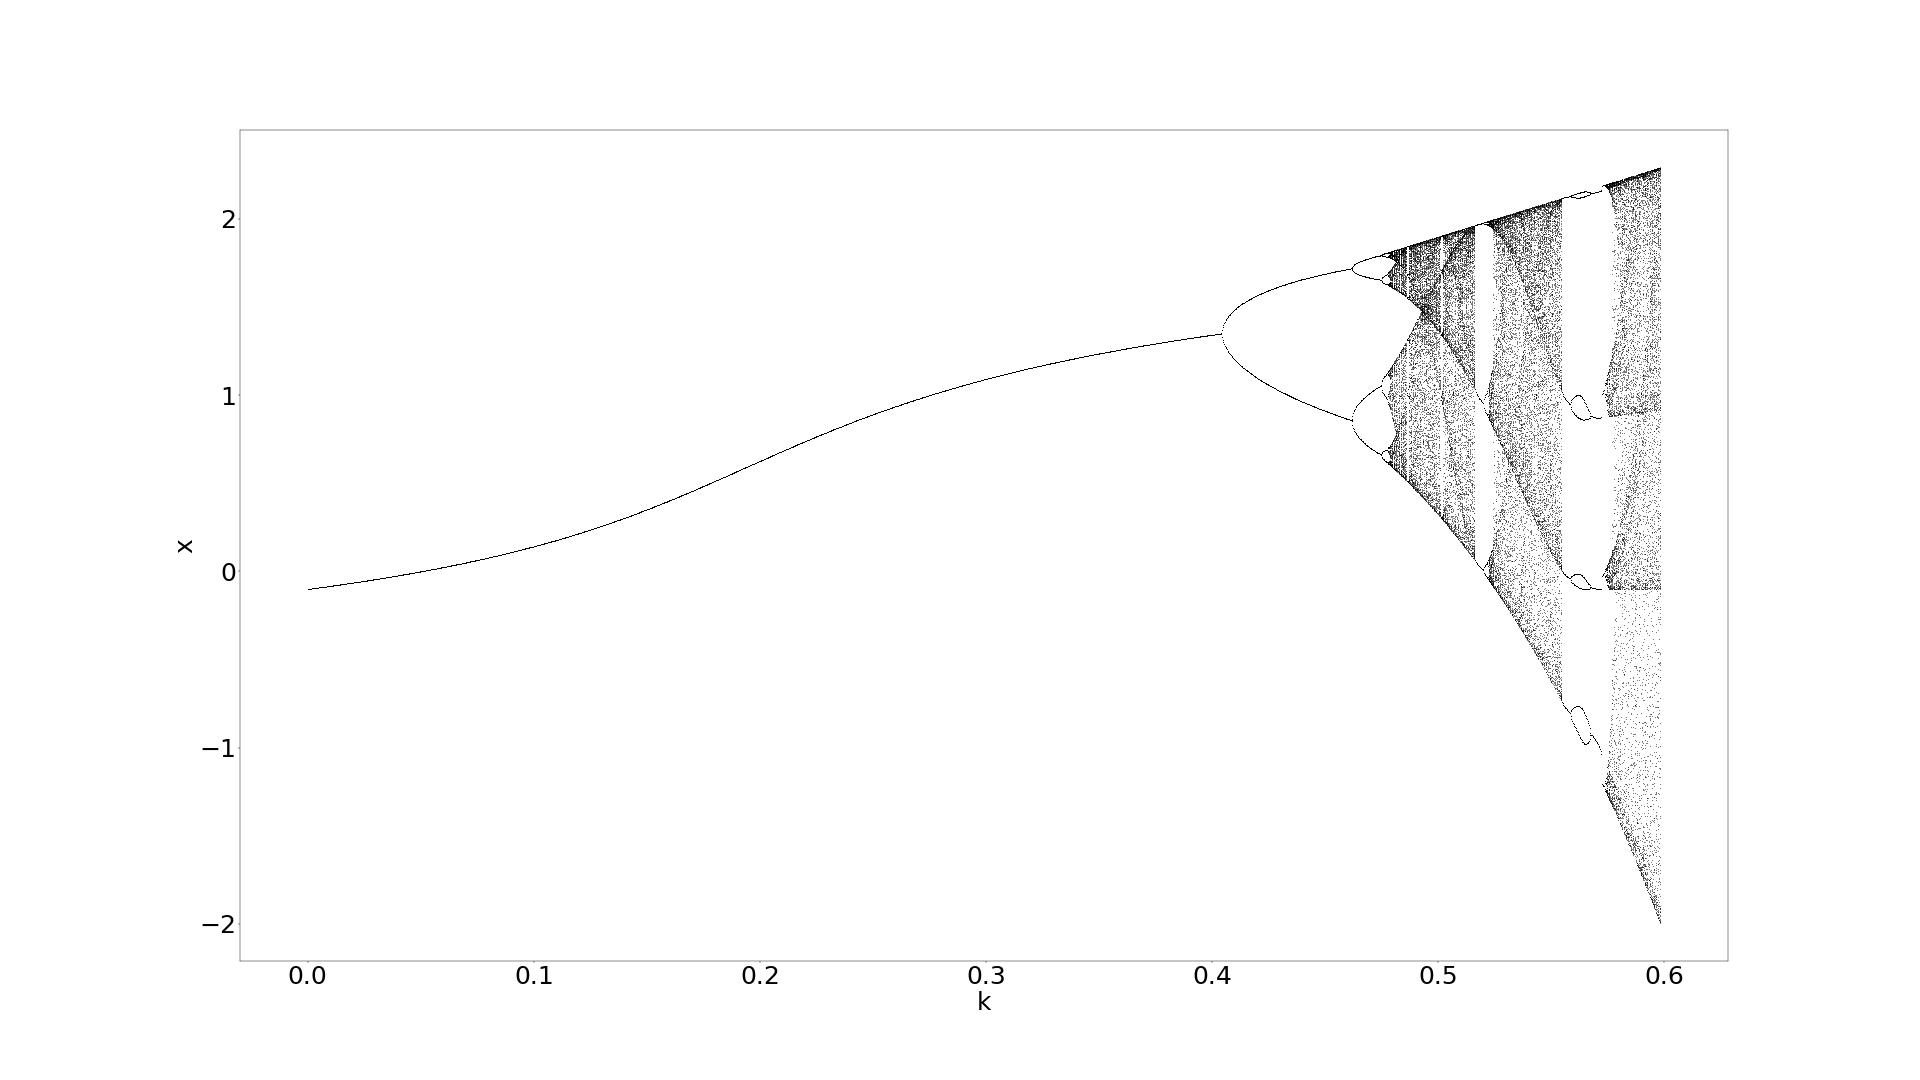
\includegraphics[width=1\linewidth]{LateX images/graphs/g1}
	\caption{ Διάγραμμα διακλάδωσης.}
	\label{th:g1}	
\end{figure}

\clearpage

\section{Φαινόμενα Χαοτικών Συστημάτων}
Τα φαινόμενα που θα αναλυθουν παρακάτω παρατηρήθηκαν στα συστήματα που μελετήθηκαν στα επόμενα κεφάλαια.

\subsection{Διπλασιασμός Περιόδου}

Αυτό το φαινόμενο παρατηρείται σε χαοτικά συστήματα όπως η λογιστική απεικόνιση. Ουσιαστικά οι διακλαδώσεις σε ένα διάγραμμα όπως στο Σχ. \ref{th:g1} όσο αυξάνεται η παράμετρος k διπλασιάζονται απο περίοδο-1 σε περίοδο-2 μέχρι που για συγκεκριμένο k το σύστημα εισέρχεται σε χάος \cite{b5}.

\subsection{Υστέρηση}
Όταν μεταξύ των ορίων διαφόρων περιοδικών περιοχών υπάρχει ασυνέχεια, τότε αυτό ονομάζεται φαινόμενο υστέρησης.

\subsection{Κρίση Ελκυστών}

Όταν παρατηρούμε μία απότομη ασυνεχή μεταβολή σε ένα χαοτικό ελκυστή
ενώ μεταβάλλεται μία παράμετρος του συστήματος,το ονομάζουμε κρίση ελκυστών. 
Οι ασυνεχείς μεταβολές είναι τυπικά τριών τύπων \cite{b5} :
\begin{enumerate}
	\item Ένας χαοτικός ελκυστής καταστρέφεται καθώς η παράμετρος περνά από μια κρίσιμη τιμή.Το είδος αυτής της κρίσης ονομάζεται συνοριακή κρίση (boundary crisis).
	\item Το μέγεθος του χαοτικού ελκυστή στο χώρο των φάσεων αυξάνεται ξαφνικά καθώς η παράμετρος περνά από την κρίσιμη τιμή της. Το είδος αυτής της κρίσης ονομάζεται
	εσωτερική κρίση, καθώς ο ελκυστής συγκρούεται με μία περιοδική τροχιά στο εσωτερικό της δεξαμενής έλξης του.
	\item Δύο ή περισσότεροι ελκυστές συγχωνεύονται για να σχηματίσουν ένα χαοτικό ελκυστή. 
\end{enumerate}
Το αντίστροφο αυτών των διαδικασιών επίσης συμβαίνουν καθώς η παράμετρος ελέγχου περνά από την κρίσιμη τιμή, κατά την αντίθετη κατεύθυνση.

\subsection{Aντιμονοτονικότητα}
Το φαινόμενo της αντιμονοτονικοτητας μπορει να εμφανιστεί με δύο τρόπους \cite{b5} :
\begin{enumerate}
	
	\item Μπορεί να παρατηρηθεί σε ένα διάγραμμα διακλάδωσης κατά την αύξηση της παραμέτρου k όταν το σύστημα ενώ μπαίνει με διπλασιασμό περιόδου στο χάος, στη συνέχεια εξέρχεται από αυτό με μία ανάστροφη ακολουθία διπλασιασμού της περιόδου και έτσι το σύστημα καταλήγει στην αρχική περίοδο του. Το σχήμα που προκύπτει στο διάγραμμα διακλάδωσης ονομάζεται χαοτική φυσαλίδα. Αυτό μπορεί να παρατηρηθεί στο Σχ. \ref{th:g3}.
	
	\item  Καθώς μεταβάλλεται η παράμετρος k, μεταξύ δύο χαοτικών περιοχών παρατηρείται μια ανάστροφη ακολουθία διπλασιασμού της περιόδου μέχρι να φτάσει σε περίοδο-1 και στη συνέχεια με διπλασιασμό της περιόδου καταλήγει πάλι στο χάος.Αυτό μπορεί να παρατηρηθεί στο Σχ. \ref{th:g4}.
	
\end{enumerate}


\subsection{Συνύπαρξη ελκυστών}
Το φαινόμενο της συνύπαρξης ελκυστών είναι το φαινόμενο κατά το οποίο το σύστημα για διαφορετικές αρχικές συνθήκες παρουσιάζει εντελώς διαφορετική δυναμική συμπεριφορά \cite{b5}.

\begin{figure}[ht]
	\centering
	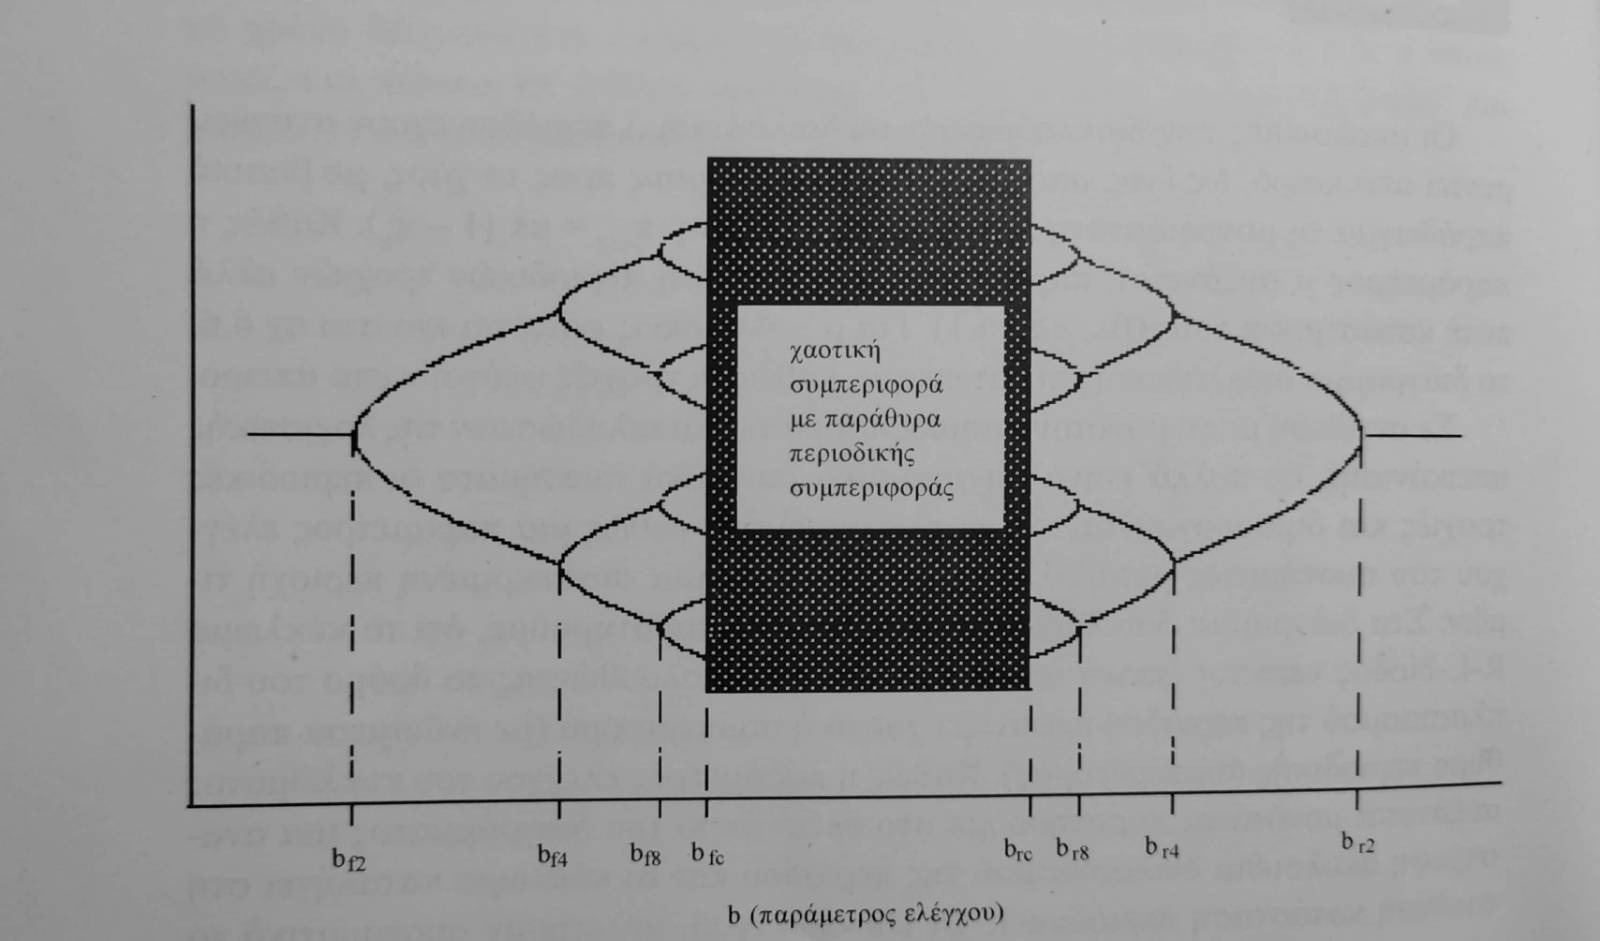
\includegraphics[width=1\linewidth]{LateX images/antimon1}
	\caption{ Σχηματικό διάγραμμα φυσαλίδας περιόδου-1.}
	\label{th:g3}	
\end{figure}

\begin{figure}[ht]
	\centering
	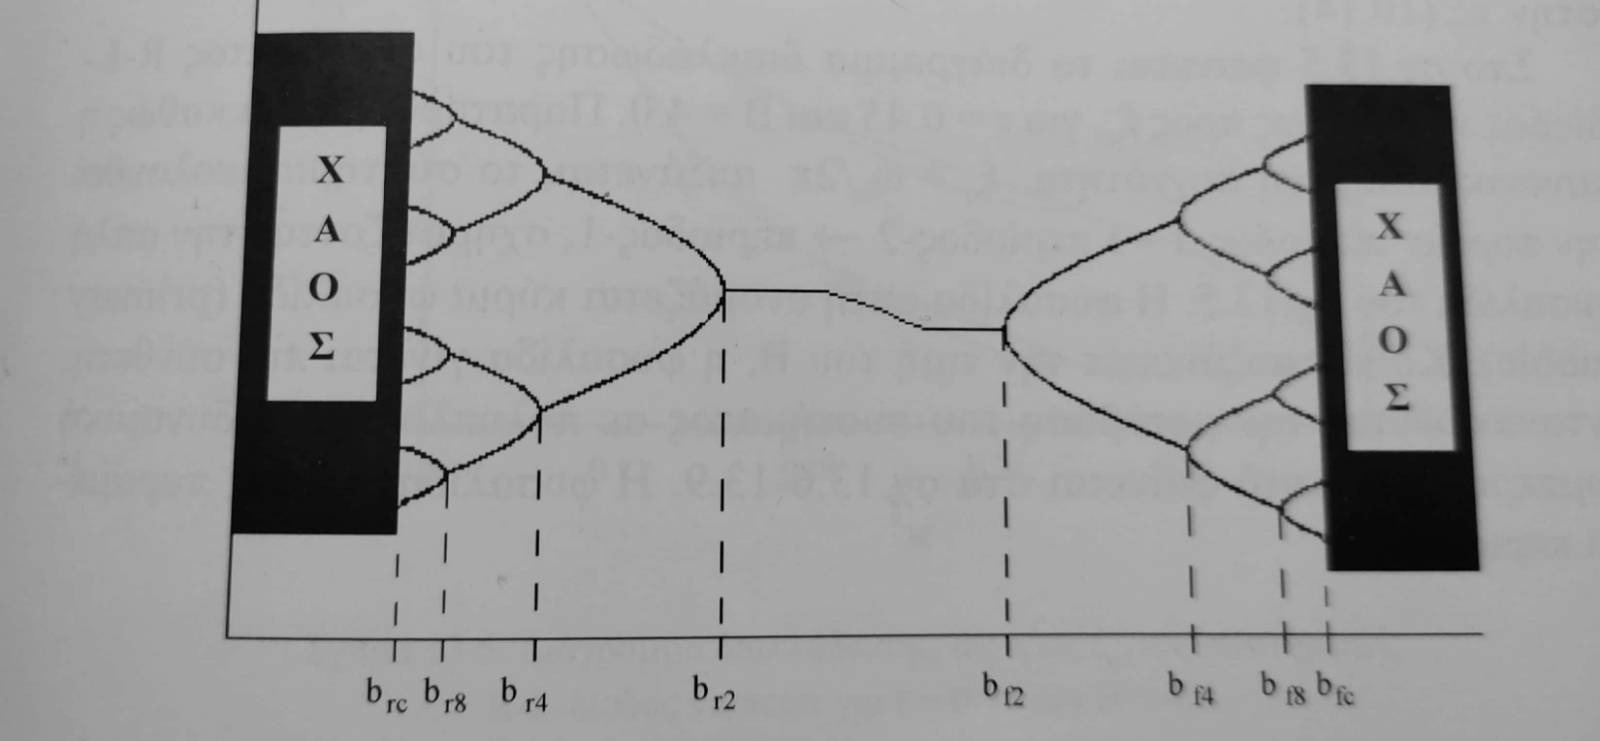
\includegraphics[width=1\linewidth]{LateX images/antimon2}
	\caption{ Σχηματικό διάγραμμα ανάστροφης φυσαλίδας περιόδου-1.}
	\label{th:g4}	
\end{figure}
\clearpage

	
	\chapter{Παραλλαγή του Λογιστικού Χάρτη}
	\label{chap:kef2}
	
\section{Παραλλαγή του Logistic Χάρτη}


Μελετήθηκε η δυναμική συμπεριφορά της εξίσωσης διακριτού χρόνου:

	\begin{equation}
		x_i=k*(a+x_{i-1})^2 *(b-x_{i-1}))
		\label{f:x1}
	\end{equation}


	όπου a,b,k, q:παράμετροι\\\\
	
	Για την εύρεση της δυναμικής συμπεριφοράς του συστήματος εξετάστηκε μια περιοχή τιμών των συγκεκριμένων παραμέτρων, ώστε να επιτευχθεί ταυτόχρονη σύγκριση της περιοδικής και χαοτικής συμπεριφοράς του. Πιο συγκεκριμένα, στη μελέτη που πραγματοποιήθηκε οι παράμετροι a, b, κρατήθηκαν αρχικά σταθερές με τιμές a=1, b=2  όπως και η αρχική συνθήκη του x1 =0.1 παρέμεινε  σταθερή,  ενώ η τιμή της παραμέτρου q μεταβάλλονταν στο διάστημα[0.1,1.7] με βήμα 0.2. Έτσι, για κάθε περίπτωση παράχθηκαν το διάγραμμα διακλάδωσης, ο εκθέτης Lyapunov και το διάγραμμά της τιμής xi σε συνάρτηση με την τιμή xi-1., τα οποία παρουσιάζονται και αναλύονται στη συνέχεια.
	
\subsection{Για q=-0.1}


	
Στο σχήμα \ref{f:g1} παρατίθεται το διάγραμμα διακλάδωσης του συστήματος \ref{f:x1}, ως προς την παράμετρο k, για a=1, b=2 και q =- 0.1. Για αυτές τις τιμές των παραμέτρων το σύστημα ξεκινάει από περίοδο-1 για k = 0.3 , ενώ για  k = 0.4 εμφανίζει τον πρώτο διπλασιασμό της περιόδου. Τον δεύτερο διπλασιασμό τον εμφανίζει για k=0.47 (περίοδος-4) ,τον τρίτο για k=0.476(περίοδος-8) . Ενώ ο τελευταίος διπλασιασμός εμφανίζεται λίγο πιο μετά τον τρίτο για k=0.478 (περίοδος-16). Στην συνέχεια για k>0.479το σύστημα εισέρχεται στο χάος , μέχρι να εξέλθει  για k=0.51(περίοδος-3) και να ξανά εισέλθει σε χάος μετά από δύο διπλασιασμούς k=0.52(περίοδος-6) και k=0.522(περίοδος-11) για k>0.524. To φαινόμενο αυτό είναι γνωστό ως συνοριακή κρίση .Εξέρχεται για τελευταία φορά από το χάος για k=0.555 (περίοδος-4). Για k=0.559 εμφανίζεται ένας διπλασιασμός (περίοδος-8) ο οποίος καταστρέφεται για k=0.567 , οπότε εδώ παρατηρούμε αντιμονοτονικότητα δηλαδή έχουμε μία ανάστροφη ακολουθία διπλασιασμού της περιόδου για k=0.568. Λόγω αυτού του φαινομένου το οποίο συνεχίζει μέχρι το q=-0.2,μελετήθηκε περαιτέρω το σύστημα από -0.1<q<-0.2.Τέλος για k=0.5735 έχουμε έναν τελευταίο διπλασιασμό(περίοδος-6) πριν ξανά εισέλθει το σύστημα για k>0.575 στο χάος.
Στο σχήμα \ref{f:g2} παρατίθενται 3 διαγράμματα διακλάδωσης \ref{f:g3}, \ref{f:g4}, \ref{f:g5}, \ref{f:g6}
για 0.54<k<0.6. Ουσιαστικά εστιάστηκε το διάγραμμα στην αντιμονοτονικότητα που εμφανίζεται για τις συγκεκριμένες τιμές του q. Επίσης παρατηρούμε στα διαγράμματα \ref{f:g4}, \ref{f:g5}, \ref{f:g6} δημιουργία χαοτικών φυσαλίδων. Δηλαδή, το σύστημα εισέρχεται στο χάος με διπλασιασιασμό της περιόδου και στην συνέχεια εξέρχεται από αυτό με αντίστροφο διπλασιασμό της περιόδου. Επιπλέον στο διάγραμμα \ref{f:g6} το φαινόμενο εμφανίζεται δυο φορές  για 0.560<k<0.568 και 0.571<k<0.573. 
Επιπλέον, στο σχήμα \ref{f:g7} παρατίθεται το διάγραμμα των εκθετών Lyapunov για τιμές του k στο ίδιο διάστημα τιμών [0.3, 0.6].  Στο διάστημα τιμών   k=0.522 , στο 0.51<k<0.522, και στο 0.554<k<0.574 παρατηρούμε ότι ο εκθέτης Lyapunov είναι συνεχώς αρνητικός, γεγονός που επιβεβαιώνει την περιοδική συμπεριφορά του συστήματος. Ενώ στα υπόλοιπα διαστήματα ο θετικός εκθέτης Lyapunov υποστηρίζει την χαοτική του συμπεριφορά, όπως έγινε φανερό και από το διάγραμμα διακλάδωσης.
Τέλος, στον Πίνακα \ref{tab:abc} παρατίθενται ενδεικτικές τιμές της παραμέτρου k και η συμπεριφορά που παρουσιάζει το σύστημα για αυτές, σύμφωνα με το διάγραμμα διακλάδωσης, καθώς και τα αντίστοιχα σχήματα των διαγραμμάτων της τιμής \(x_i\) σε συνάρτηση με την τιμή \(x_{i+1}\). Από τα παραγόμενα σχήματα προκύπτει αριθμός σημείων αντίστοιχος με την περίοδο του συστήματος.


\begin{table}[h!]
	\centering
	\begin{tabular}{l | l | l}
		Παράμετρος k & Συμπεριφορά & Σχήμα\\
		\hline
		0.3 &  Περίοδος-1 & \ref{f:k1}\\
		0.41 & Περίοδος-2 & \ref{f:k2}\\
		0.476 &  Περίοδος-8 & \ref{f:k3}\\
		0.4778 & Περίοδος-16 & \ref{f:k4}\\
		0.479 & Χάος & \ref{f:k5}\\
		0.517 & Περίοδος-3 & \ref{f:k6})\\
		0.52 & Περίοδος-6 & \ref{f:k7}\\
		0.522 & Περίοδος-11 & \ref{f:k8}\\
		0.524 & Χάος & \ref{f:k9}\\
		0.555 & Περίοδος-4 & \ref{f:k10}\\
		0.559 & Περίοδος-8 & \ref{f:k11}\\
		0.568 & Περίοδος-4 & \ref{f:k12}\\
		0.5735 & Περίοδος-6 & \ref{f:k13}\\
		0.575 & Χάος & \ref{f:k14}\\
	\end{tabular}
	\caption{ Συμπεριφορά του υπό μελέτη συστήματος για διάφορες τιμές του k,για a=1, b=2 και q=-0.1}
	\label{tab:abc}
\end{table}


\begin{figure}[h!]
	\centering
	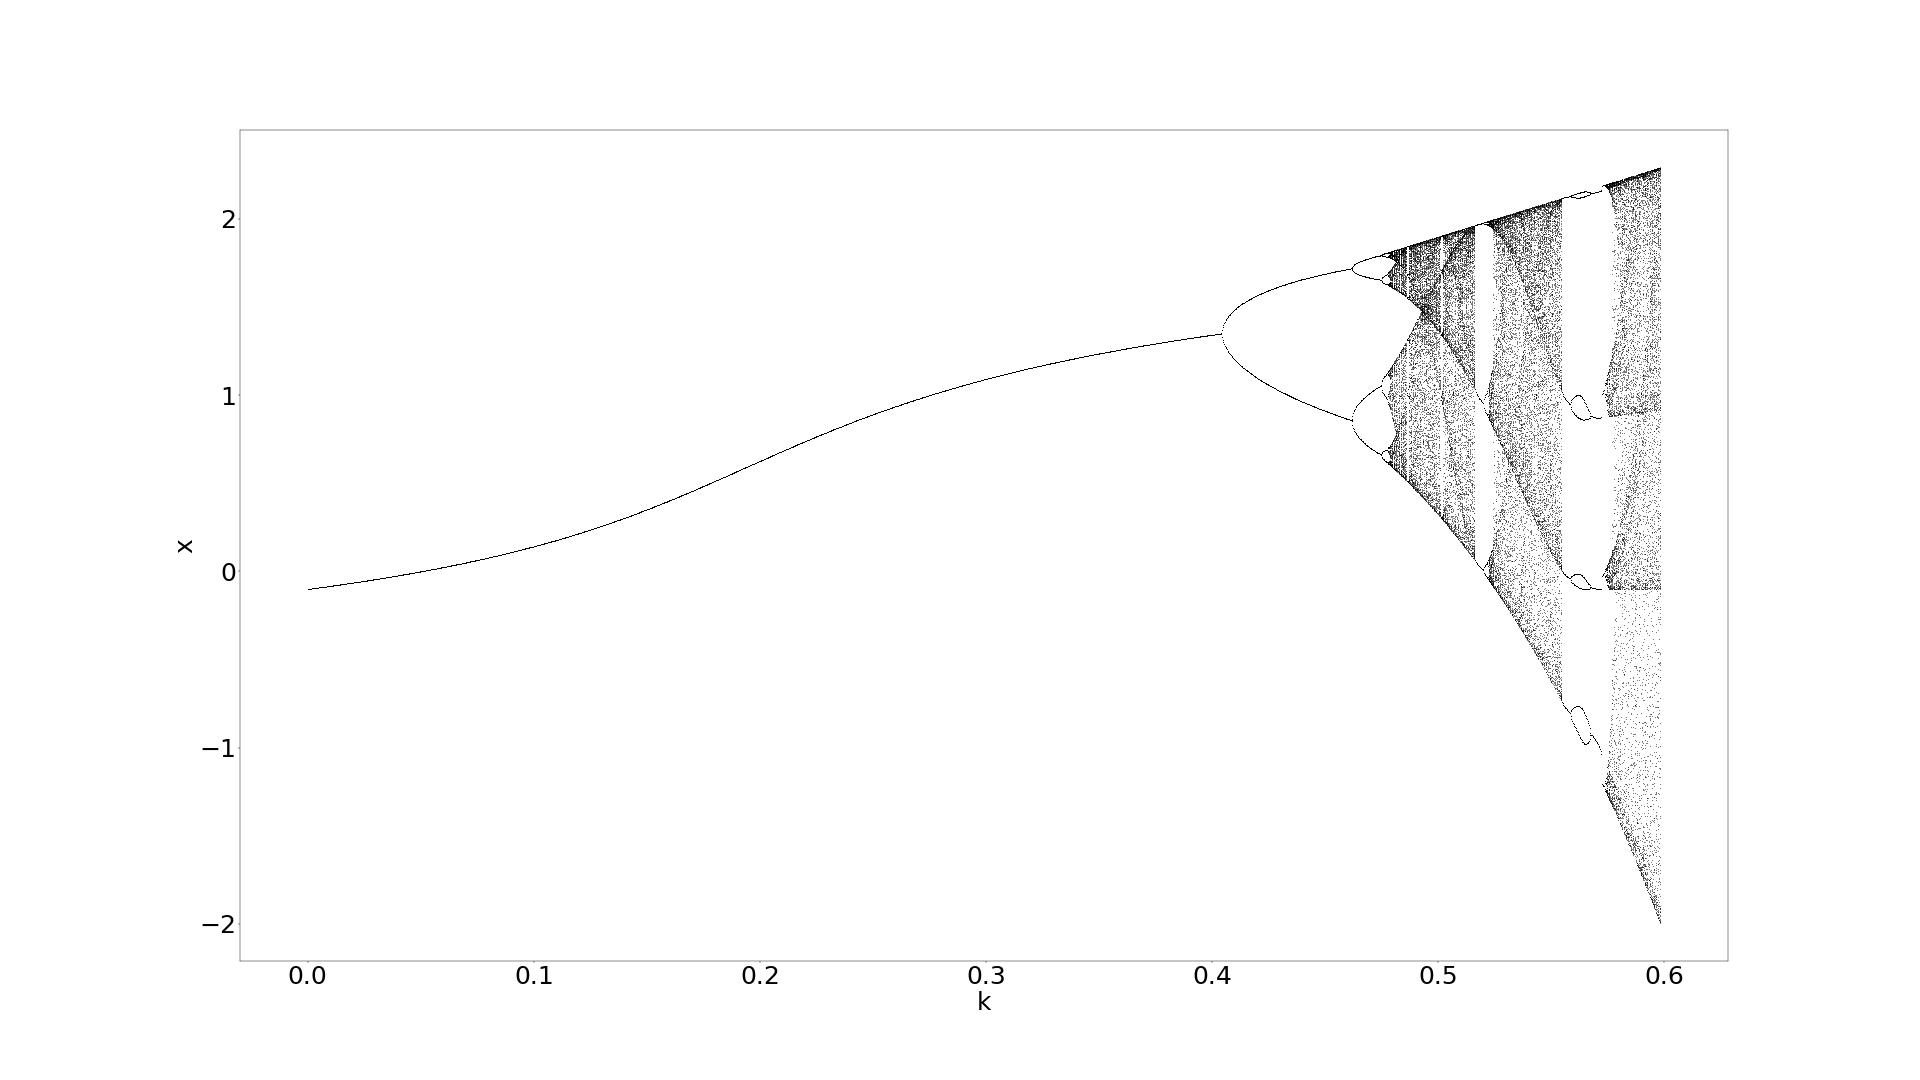
\includegraphics[width=0.6\linewidth]{LateX images/graphs/g1}
	\caption{ Διάγραμμα διακλάδωσης, για a=1, b=2 και q=-0.1}
	\label{f:g1}
\end{figure}



\begin{figure}[h!]
	\centering
	\caption{}
	\label{f:g2}
	\begin{subfigure}[b]{0.4\textwidth}
		\centering
		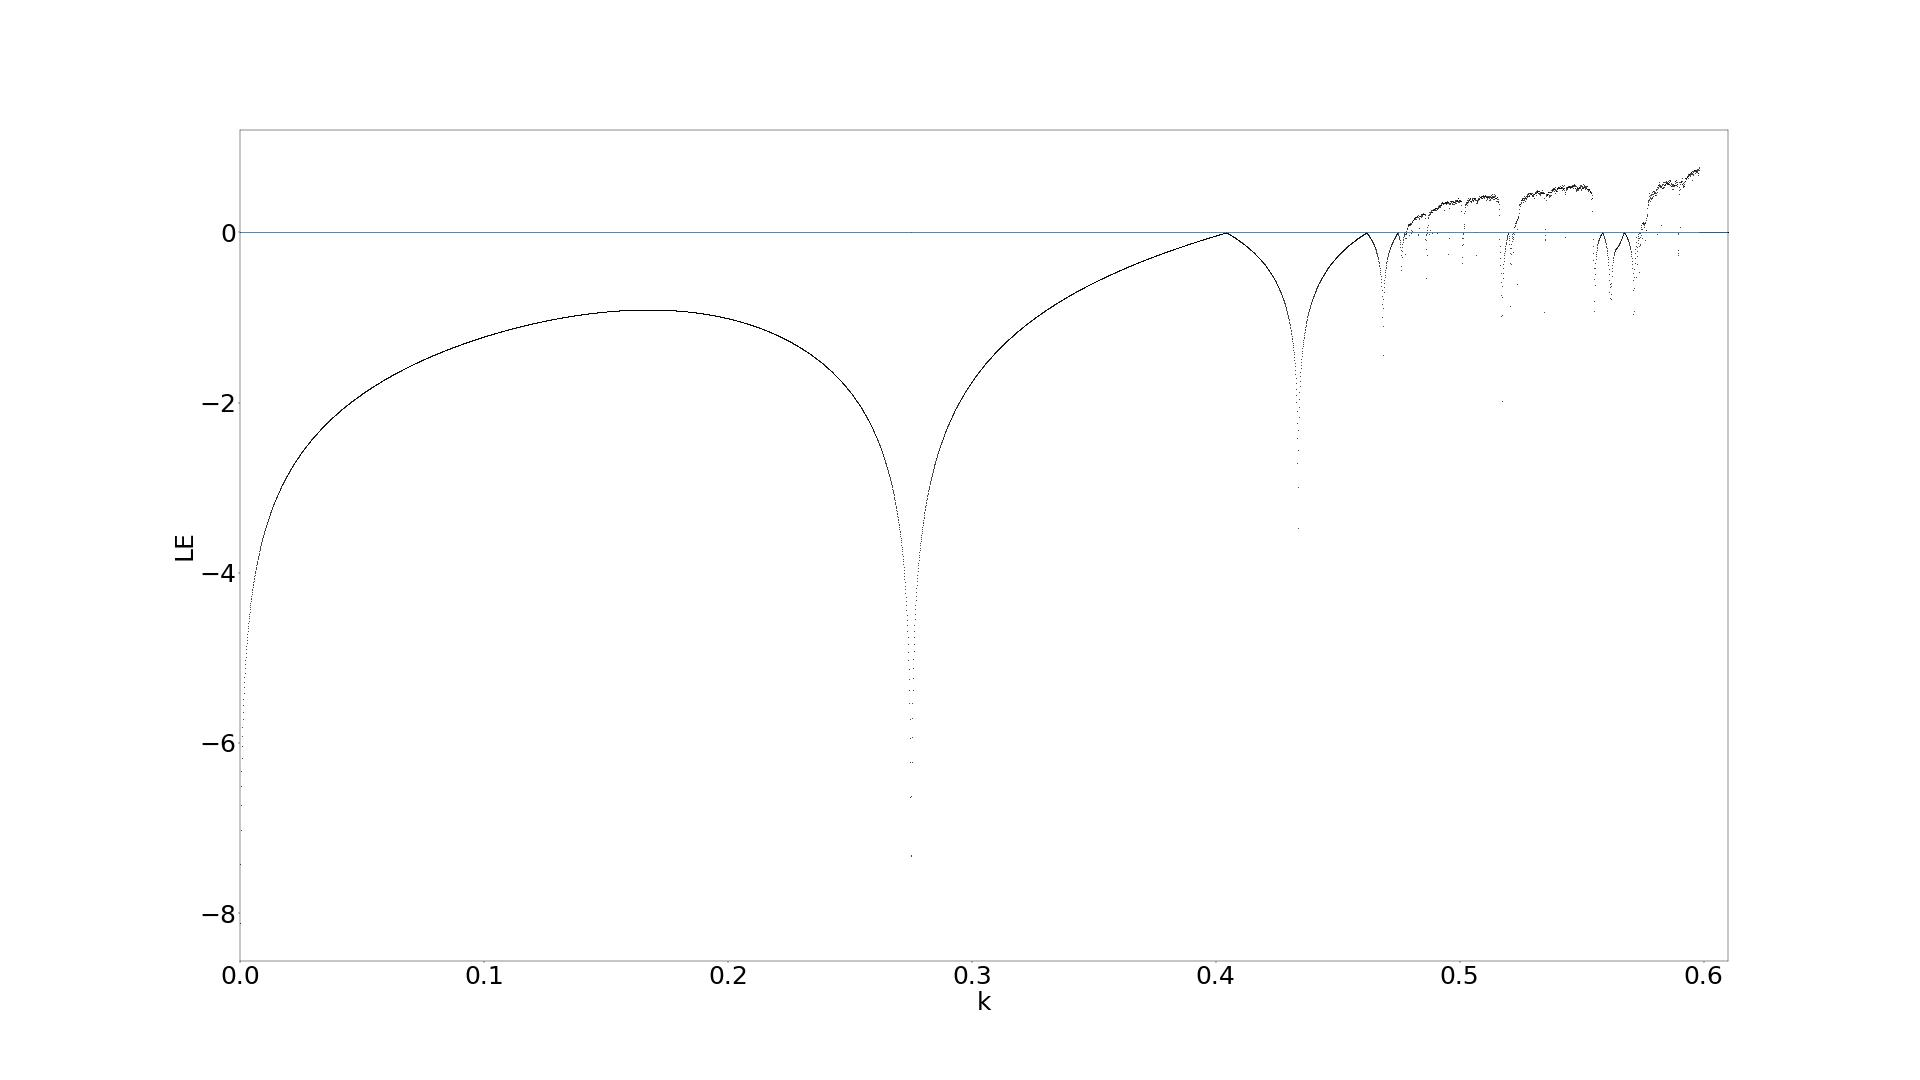
\includegraphics[width=\textwidth]{LateX images/graphs/g2}
		\caption{Διάγραμμα διακλάδωσης, για q=-0.112}
		\label{f:g3}
	\end{subfigure}
	\hfill
	\begin{subfigure}[b]{0.4\textwidth}
		\centering
		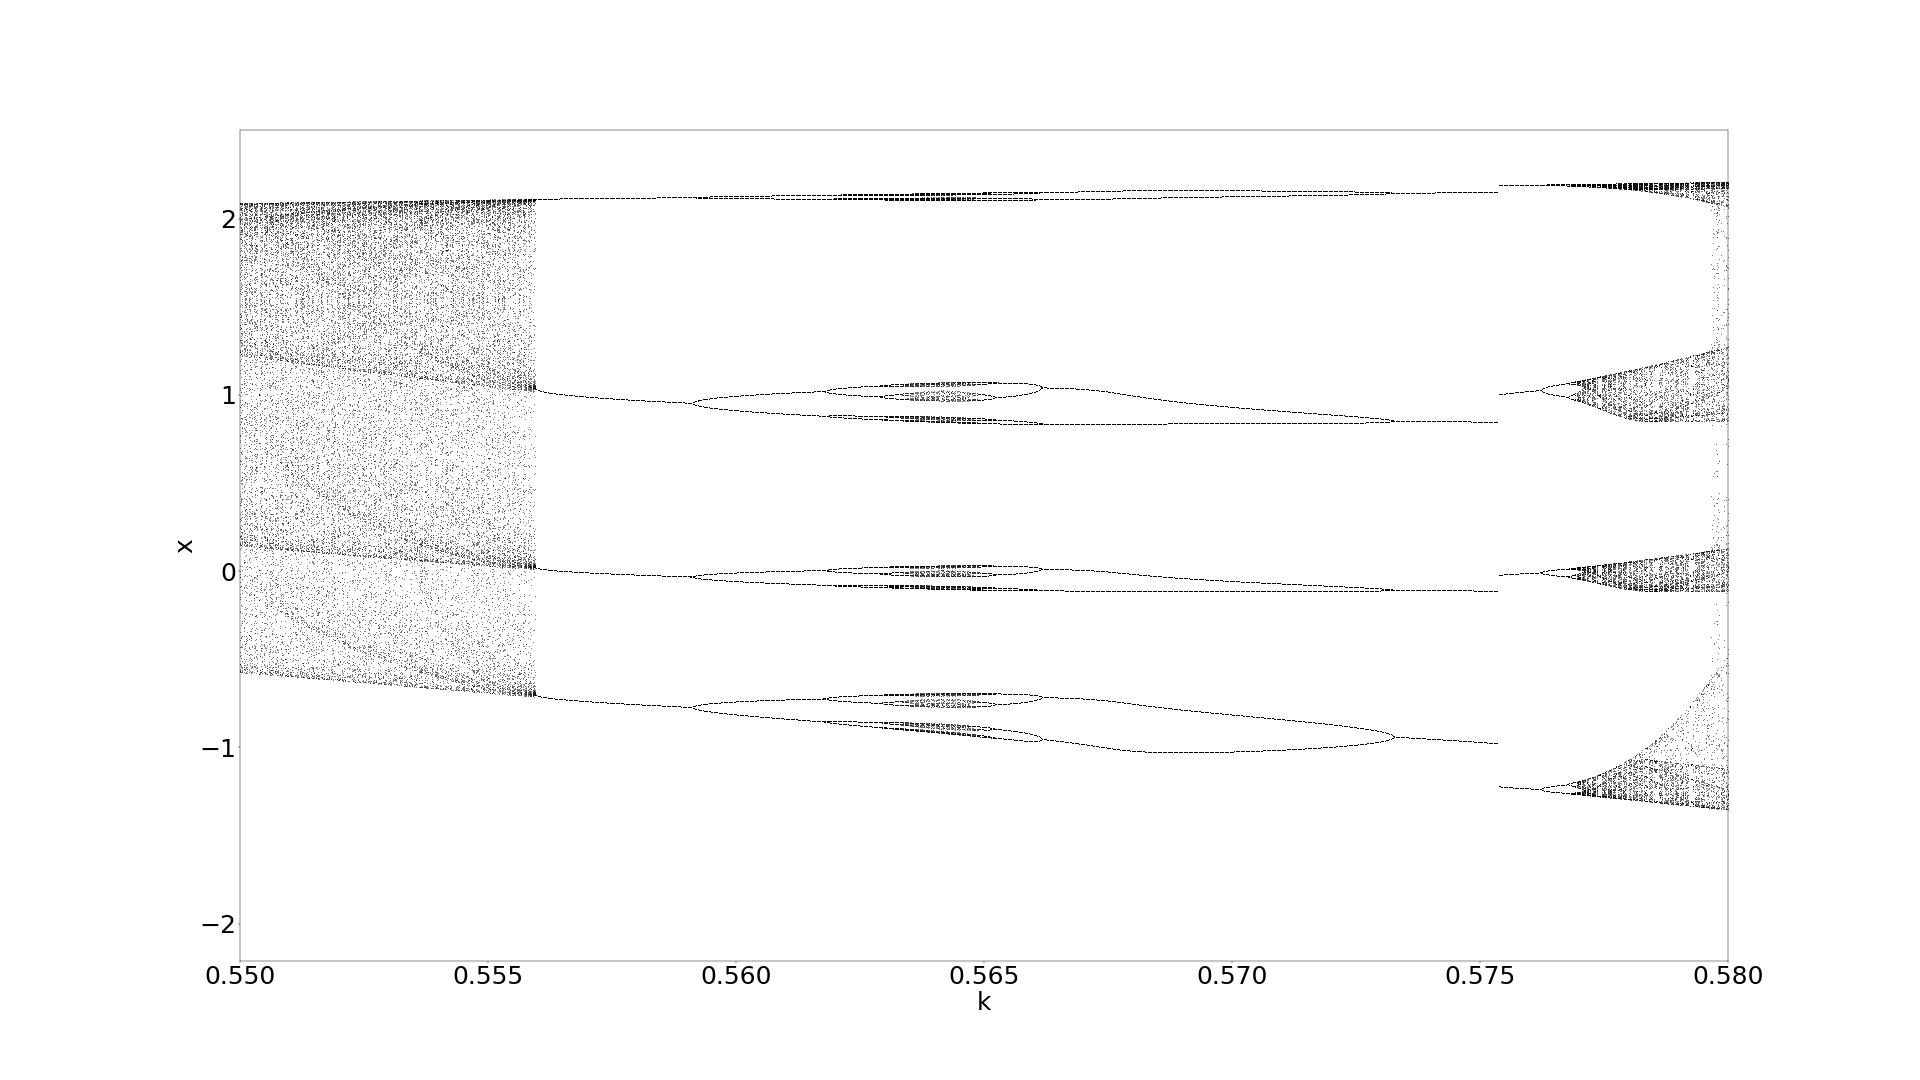
\includegraphics[width=\textwidth]{LateX images/graphs/g3}
		\caption{Διάγραμμα διακλάδωσης, για q=-0.114}
		\label{f:g4}
	\end{subfigure}
	\hfill
	\begin{subfigure}[b]{0.4\textwidth}
		\centering
		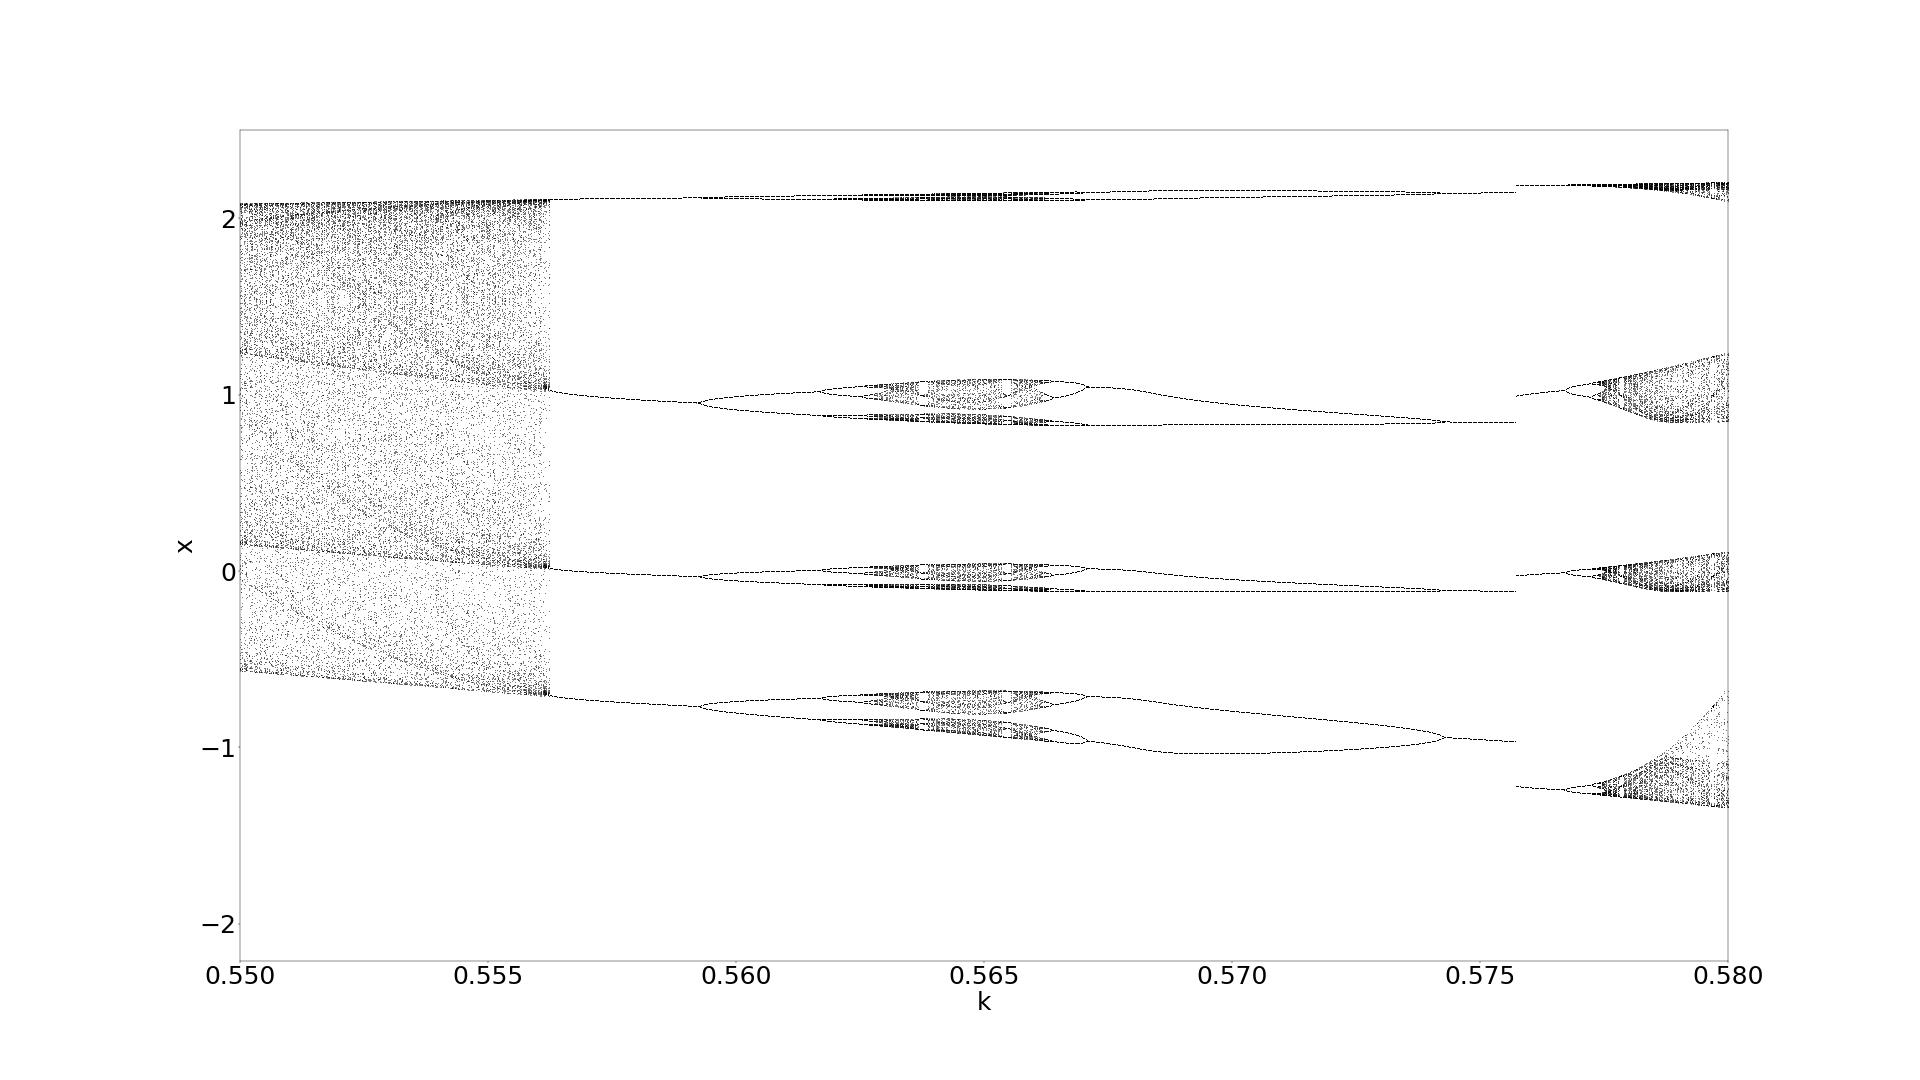
\includegraphics[width=\textwidth]{LateX images/graphs/g4}
		\caption{Διάγραμμα διακλάδωσης, για q=-0.116}
		\label{f:g5}
	\end{subfigure}
	\hfill
	\begin{subfigure}[b]{0.4\textwidth}
		\centering
		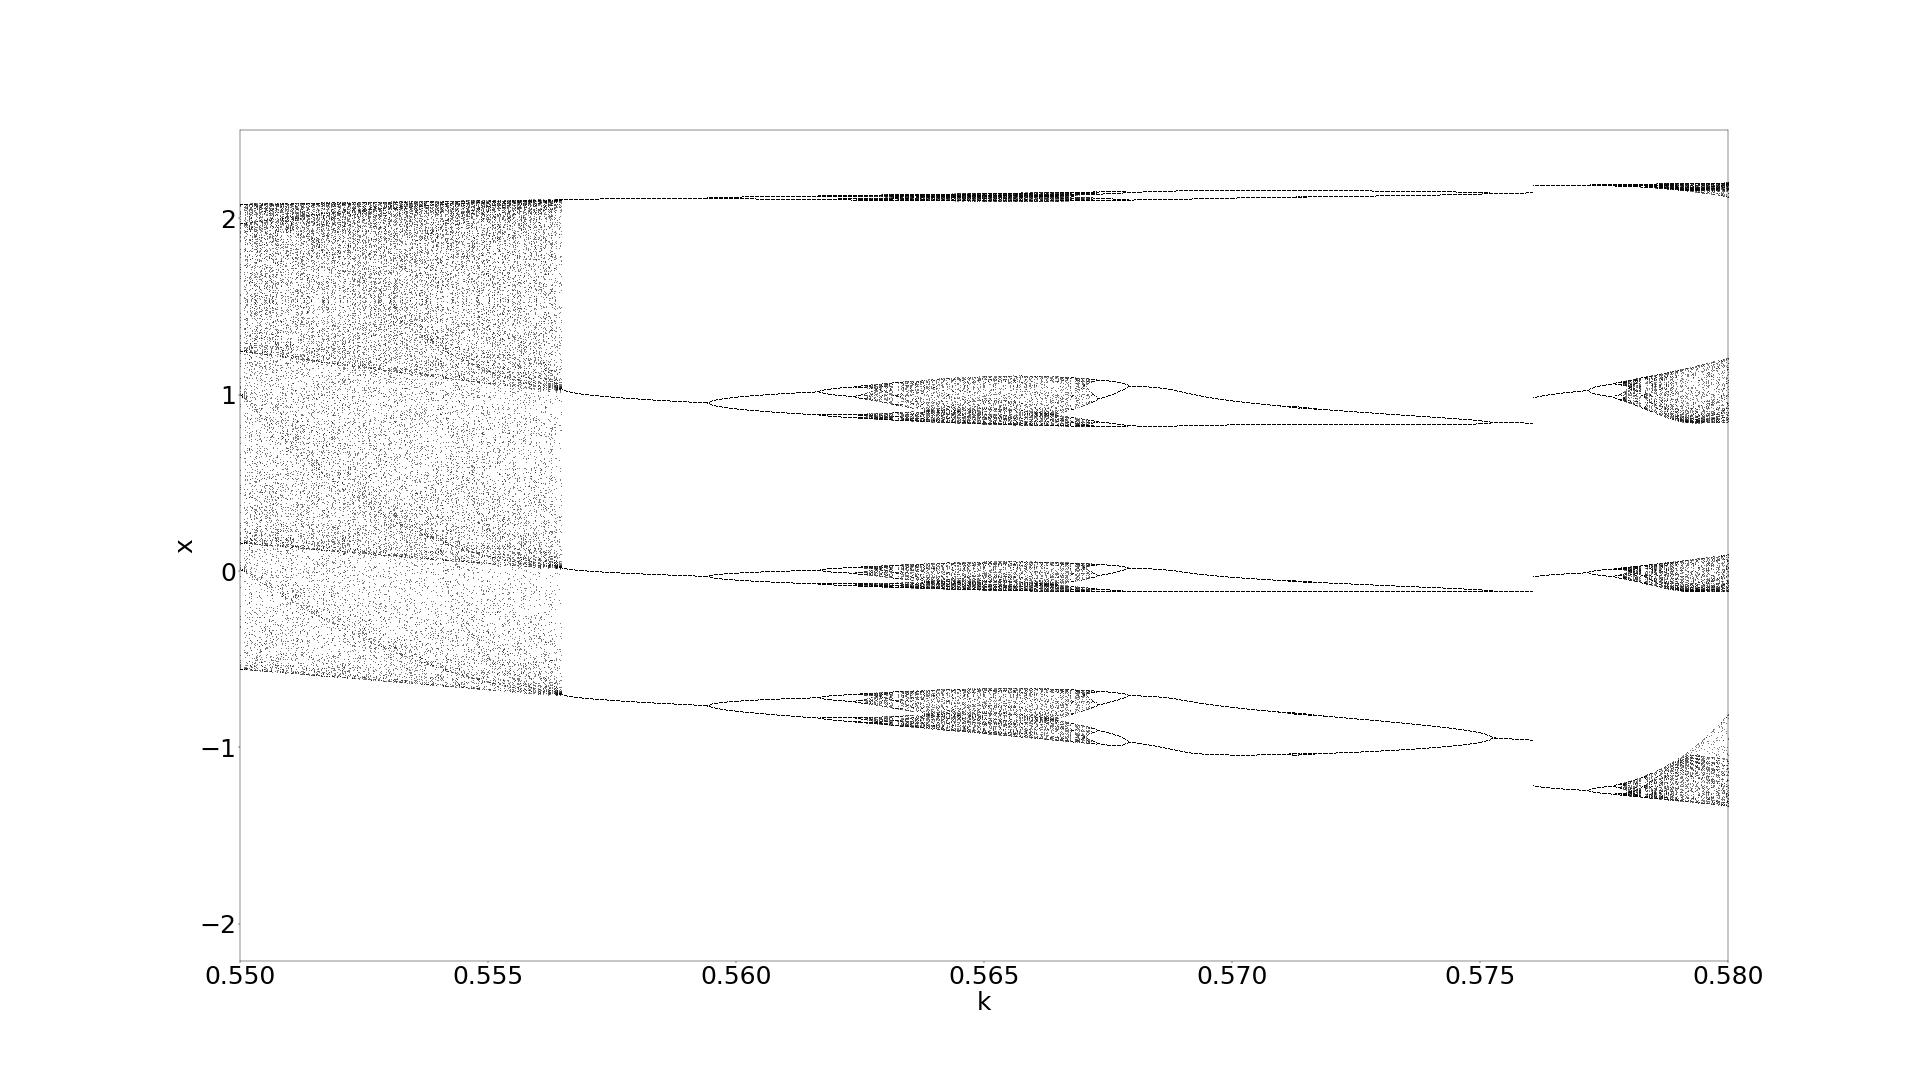
\includegraphics[width=\textwidth]{LateX images/graphs/g5}
		\caption{Διάγραμμα διακλάδωσης, για q=-0.118}
		\label{f:g6}
	\end{subfigure}
\end{figure}

\begin{figure}[h!]
	\centering
	\includegraphics[width=0.6\linewidth]{"LateX images/graphs/g6 "}
	\caption{Διάγραμμα του εκθέτη Lyapunov σε συνάρτηση με την παράμετρο k, για a=1, b=2 και q=-0.1.}
	\label{f:g7}
\end{figure}



\begin{figure}[h!]
	\centering
	\caption{Διαγράμματα της τιμής \(x_i\) με την τιμή \(x_{i+1}\) :}
	\begin{subfigure}[b]{0.25\textwidth}
		\centering
		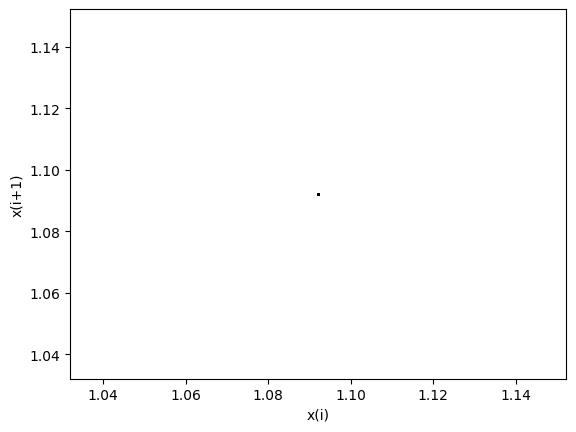
\includegraphics[width=\textwidth]{LateX images/graphs/k03}
		\caption{Για k=0.3}
		\label{f:k1}
	\end{subfigure}
	\hfill
	\begin{subfigure}[b]{0.25\textwidth}
		\centering
		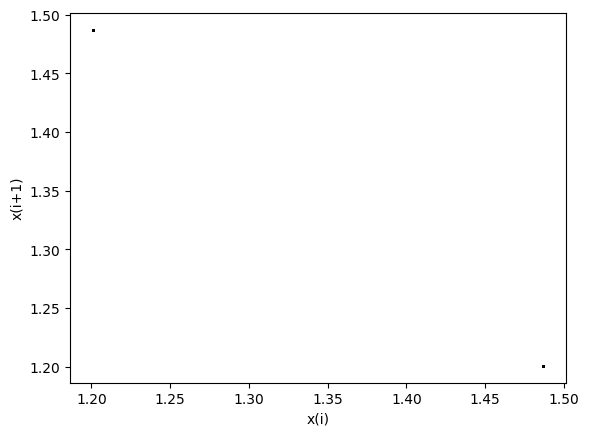
\includegraphics[width=\textwidth]{LateX images/graphs/k041}
		\caption{Για k=0.41}
		\label{f:k2}
	\end{subfigure}
	\hfill
	\begin{subfigure}[b]{0.25\textwidth}
		\centering
		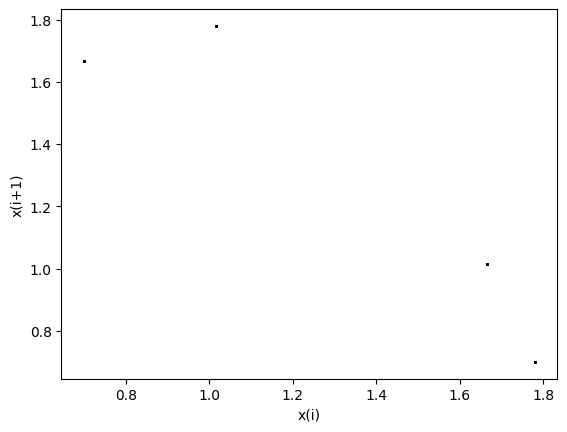
\includegraphics[width=\textwidth]{LateX images/graphs/k047}
		\caption{Για k=0.047}
		\label{f:k3}
	\end{subfigure}
	\begin{subfigure}[b]{0.25\textwidth}
		\centering
		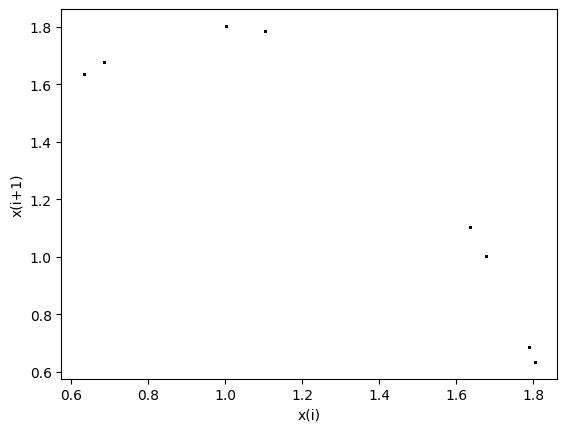
\includegraphics[width=\textwidth]{LateX images/graphs/k0476}
		\caption{Για k=0.476}
		\label{f:k4}
	\end{subfigure}
	\hfill
	\begin{subfigure}[b]{0.25\textwidth}
		\centering
		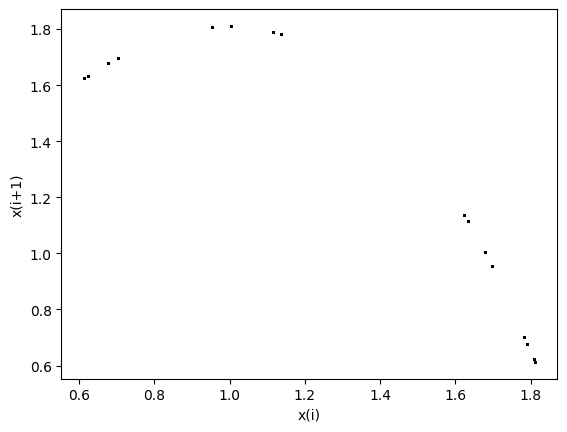
\includegraphics[width=\textwidth]{LateX images/graphs/k04778}
		\caption{Για k=0.4778}
		\label{f:k5}
	\end{subfigure}
	\hfill
	\begin{subfigure}[b]{0.25\textwidth}
		\centering
		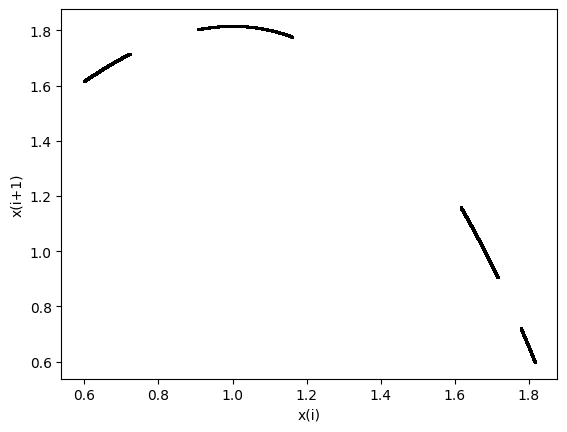
\includegraphics[width=\textwidth]{LateX images/graphs/k0479}
		\caption{Για k=0.479}
		\label{f:k6}
	\end{subfigure}
	\hfill
	\begin{subfigure}[b]{0.25\textwidth}
		\centering
		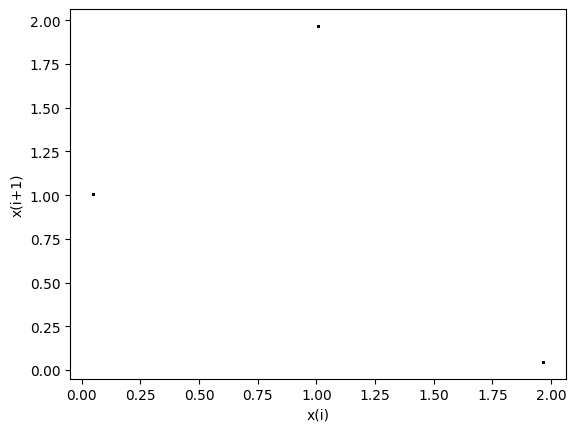
\includegraphics[width=\textwidth]{LateX images/graphs/k0517}
		\caption{Για k=0.517}
	\end{subfigure}
	\hfill
	\begin{subfigure}[b]{0.25\textwidth}
		\centering
		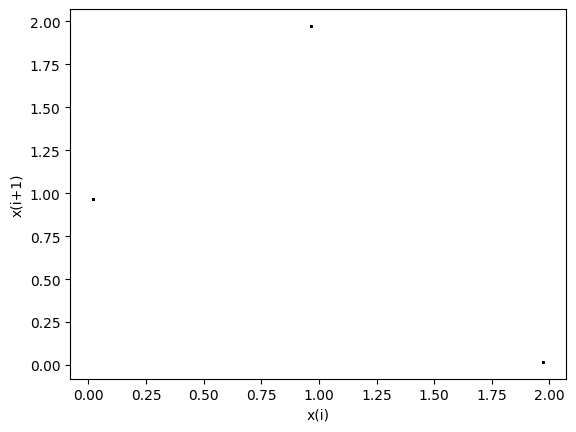
\includegraphics[width=\textwidth]{LateX images/graphs/k0519}
		\caption{Για k=0.519}
		\label{f:k7}
	\end{subfigure}
	\hfill
	\begin{subfigure}[b]{0.25\textwidth}
		\centering
		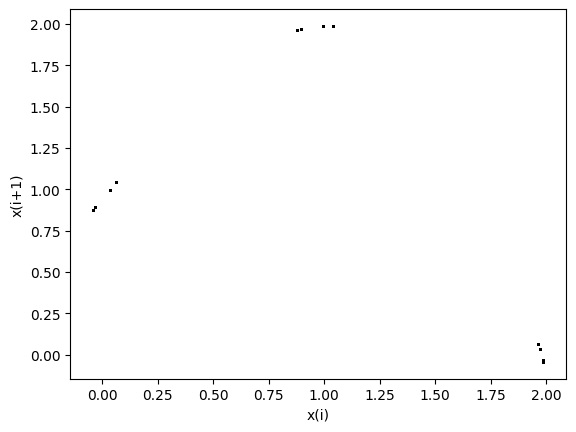
\includegraphics[width=\textwidth]{LateX images/graphs/k0522}
		\caption{Για k=0.522}
		\label{f:k8}
	\end{subfigure}
	\hfill
	\begin{subfigure}[b]{0.25\textwidth}
		\centering
		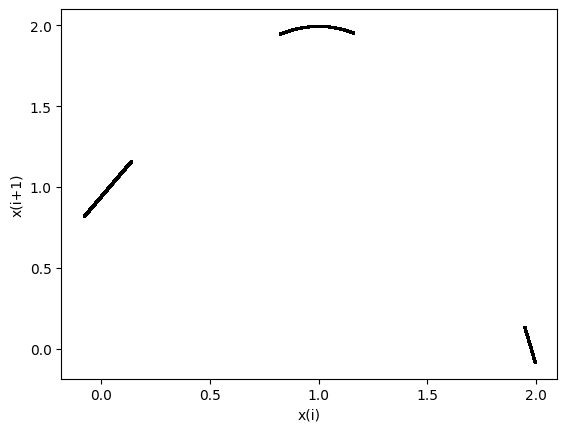
\includegraphics[width=\textwidth]{LateX images/graphs/k0524}
		\caption{Για k=0.524}
		\label{f:k9}
	\end{subfigure}
	\hfill
	\begin{subfigure}[b]{0.25\textwidth}
		\centering
		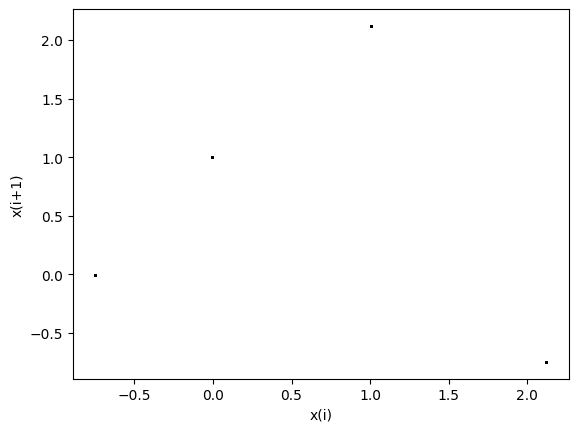
\includegraphics[width=\textwidth]{LateX images/graphs/k0555}
		\caption{Για k=0.555}
		\label{f:k10}
	\end{subfigure}
	\hfill
	\begin{subfigure}[b]{0.25\textwidth}
		\centering
		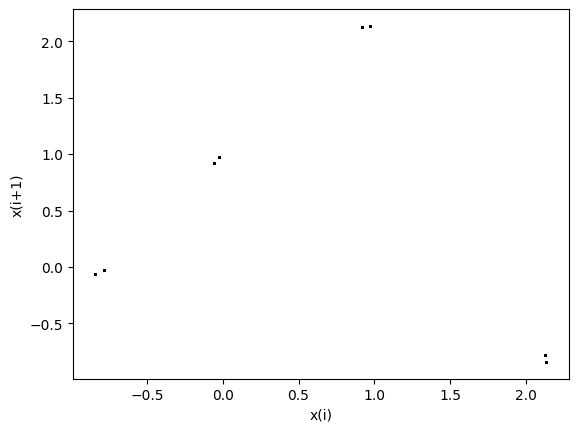
\includegraphics[width=\textwidth]{LateX images/graphs/k0559}
		\caption{Για k=0.559}
		\label{f:k11}
	\end{subfigure}
	\hfill
	\begin{subfigure}[b]{0.25\textwidth}
		\centering
		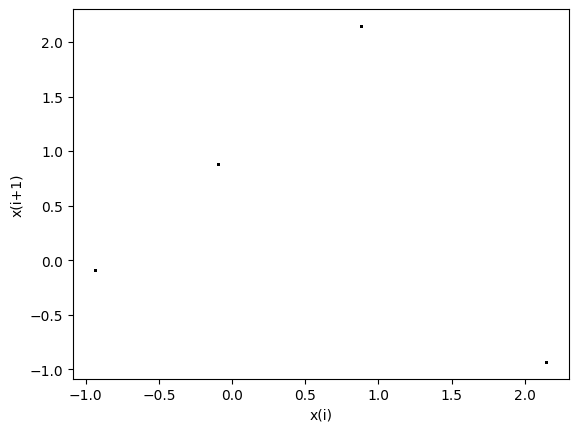
\includegraphics[width=\textwidth]{LateX images/graphs/k0568}
		\caption{Για k=0.568}
		\label{f:k12}
	\end{subfigure}
	\hfill
	\begin{subfigure}[b]{0.25\textwidth}
		\centering
		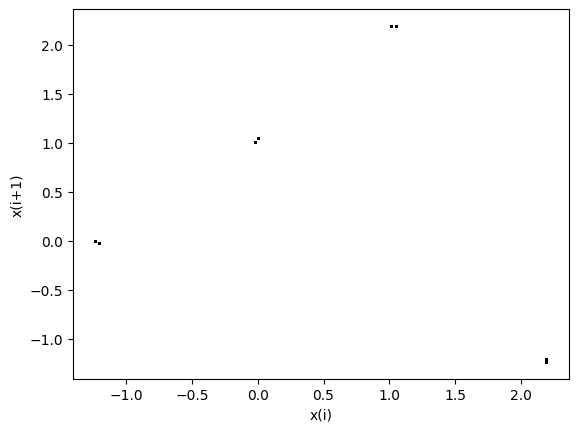
\includegraphics[width=\textwidth]{LateX images/graphs/k05735}
		\caption{Για k=0.5735}
		\label{f:k13}
	\end{subfigure}
	\hfill
	\begin{subfigure}[b]{0.25\textwidth}
		\centering
		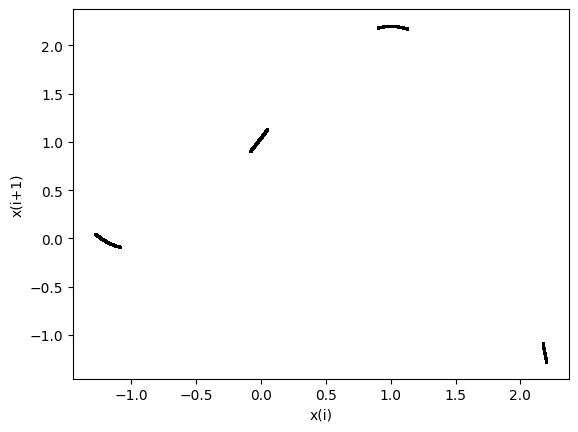
\includegraphics[width=\textwidth]{LateX images/graphs/k0575}
		\caption{Για k=0.575}
		\label{f:k14}
	\end{subfigure}

\end{figure}

 \clearpage
\subsection{Για q=-0.3}

Στο σχήμα \ref{f:g8} παρατίθεται το διάγραμμα διακλάδωσης του συστήματος \ref{f:x1}, ως προς την παράμετρο k, για a=1, b=2 και q =- 0.3. Για αυτές τις τιμές των παραμέτρων το σύστημα ξεκινάει από περίοδο-1 για k = 0.3 , ενώ για  k = 0.44 εμφανίζει τον πρώτο διπλασιασμό της περιόδου. Τον δεύτερο διπλασιασμό τον εμφανίζει για k=0.5 (περίοδος-4) ,τον τρίτο για k=0.511(περίοδος-8).Στην συνέχεια για k>0.5165 το σύστημα εισέρχεται στο χάος , μέχρι να εξέλθει  για k=0.551(περίοδος-3) και να ξανά εισέλθει σε χάος μετά από δύο διπλασιασμούς k=0.555(περίοδος-6) και k=0.556(περίοδος-12) για k>0.5573. To φαινόμενο αυτό είναι γνωστό ως συνοριακή κρίση .Εξέρχεται για τελευταία φορά από το χάος για k=0.583 (περίοδος-4) και μετά απο ένα διπλασιασμό  για k=0.5846(Περίόδος-7) είσέρχεται για τελευταία φορά στο χάος για k=0.5851.
Επομένως και σε αυτή την περίπτωση το σύστημα εισέρχεται στο χάος με διπλασιασμό της περιόδου. 
Επιπλέον, στο σχήμα \ref{f:g9} παρατίθεται το διάγραμμα των εκθετών Lyapunov για τιμές του k στο ίδιο διάστημα τιμών [0, 0.63].  Στο διάστημα τιμών   0<k<0.511 , στο 0.551<k<0.556, και στο 0.583<k<0.5846 παρατηρούμε ότι ο εκθέτης Lyapunov είναι συνεχώς αρνητικός, γεγονός που επιβεβαιώνει την περιοδική συμπεριφορά του συστήματος. Ενώ στα υπόλοιπα διαστήματα ο θετικός εκθέτης Lyapunov υποστηρίζει την χαοτική του συμπεριφορά, όπως έγινε φανερό και από το διάγραμμα διακλάδωσης.
Τέλος, στον Πίνακα \ref{tab:abc1} παρατίθενται ενδεικτικές τιμές της παραμέτρου k και η συμπεριφορά που παρουσιάζει το σύστημα για αυτές, σύμφωνα με το διάγραμμα διακλάδωσης, καθώς και τα αντίστοιχα σχήματα των διαγραμμάτων της τιμής \(x_i\) σε συνάρτηση με την τιμή \(x_{i+1}\). Από τα παραγόμενα σχήματα προκύπτει αριθμός σημείων αντίστοιχος με την περίοδο του συστήματος.
\begin{table}[h!]
	\centering
	\begin{tabular}{l | l | l}
		Παράμετρος k & Συμπεριφορά & Σχήμα\\
		\hline
		0.3 &  Περίοδος-1 & \ref{f:k1}\\
		0.44& Περίοδος-2 & \ref{f:k2}\\
		0.5& Περίοδος-4 & \ref{f:k2}\\
		0.511 &  Περίοδος-8 & \ref{f:k3}\\
		0.5165 & Χάος & \ref{f:k5}\\
		0.551 & Περίοδος-3 & \ref{f:k6})\\
		0.555 & Περίοδος-6 & \ref{f:k7}\\
		0.556 & Περίοδος-12 & \ref{f:k8}\\
		0.5573 & Χάος & \ref{f:k9}\\
		0.583& Περίοδος-4 & \ref{f:k10}\\
		0.5846 & Περίοδος-7 & \ref{f:k11}\\
		0.5851 & Χάος & \ref{f:k14}\\
	\end{tabular}
	\caption{ Συμπεριφορά του υπό μελέτη συστήματος για διάφορες τιμές του k,για a=1, b=2 και q=-0.3}
	\label{tab:abc1}
\end{table}

\begin{figure}[h!]
	\centering
	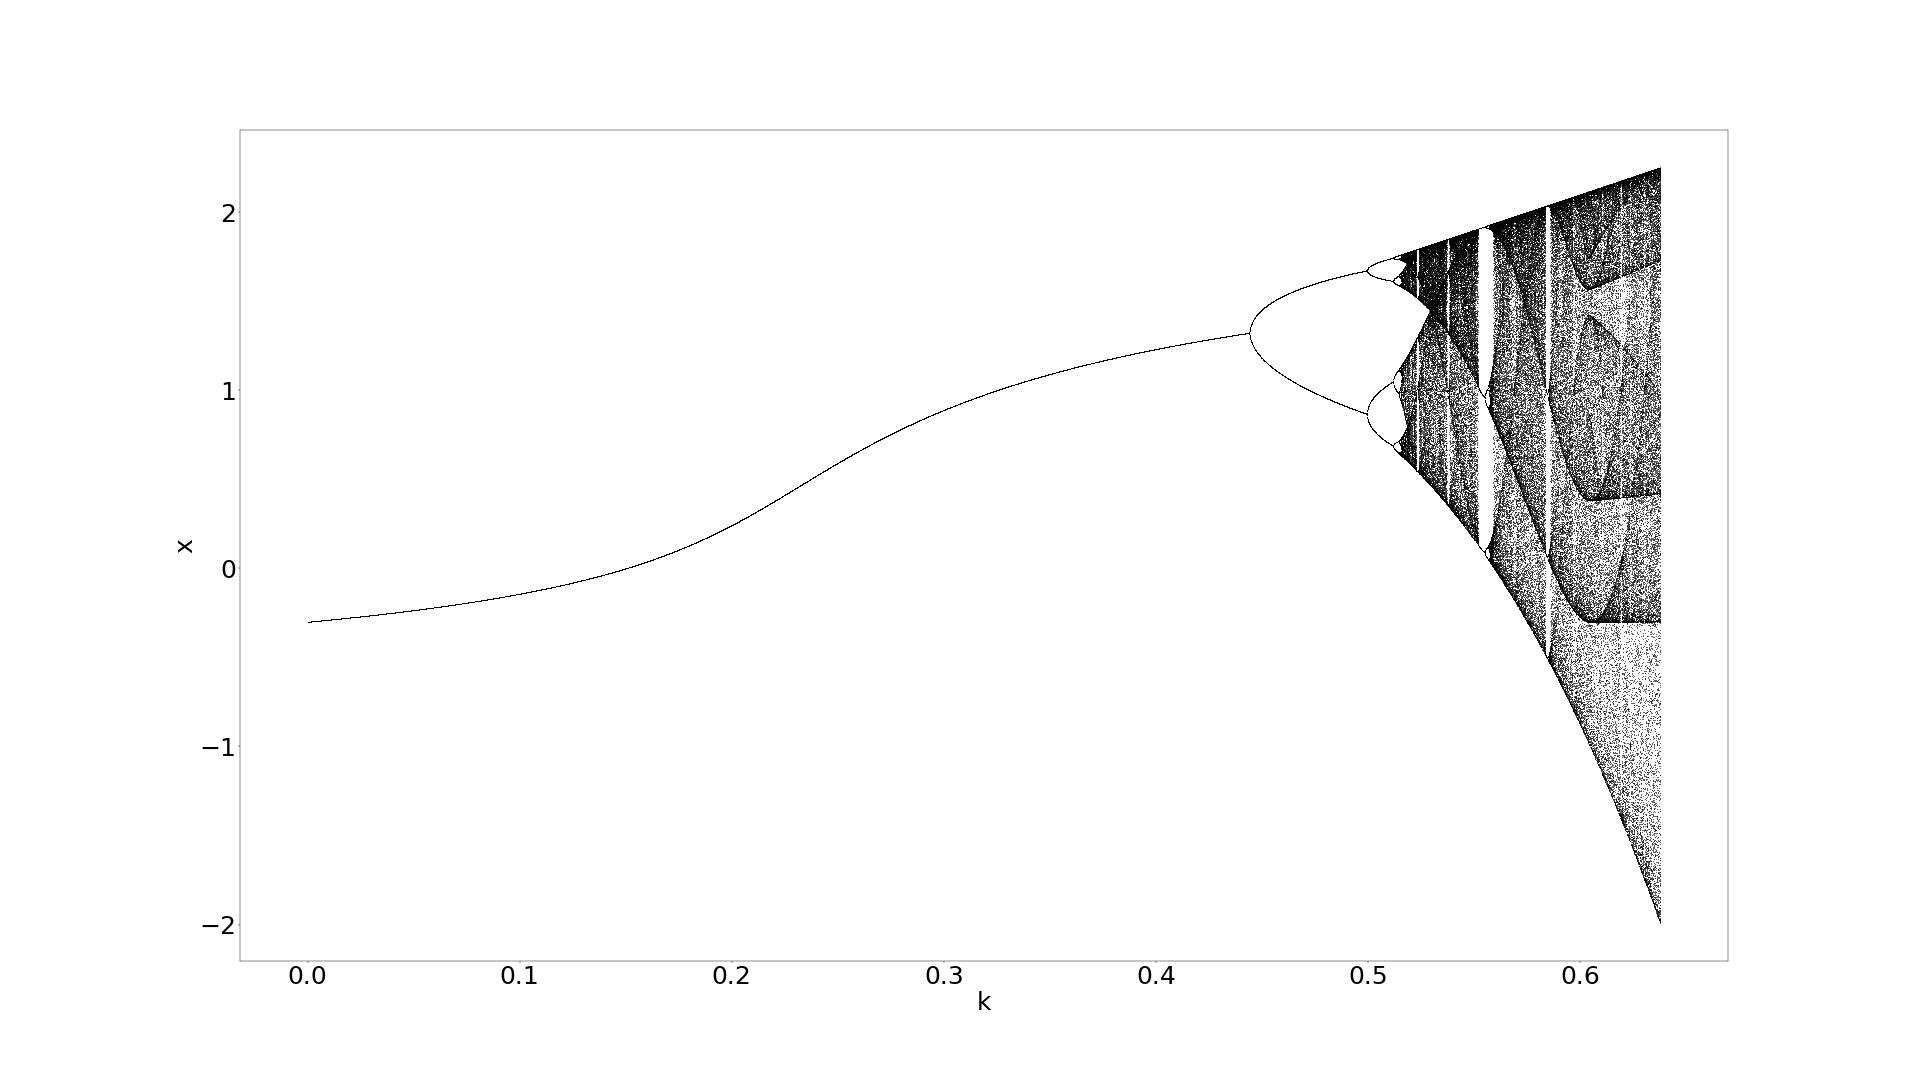
\includegraphics[width=0.6\linewidth]{LateX images/graphs q03/g1}
	\caption{ Διάγραμμα διακλάδωσης, για a=1, b=2 και q=-0.3}
	\label{f:g8}
\end{figure}

\begin{figure}[h!]
	\centering
	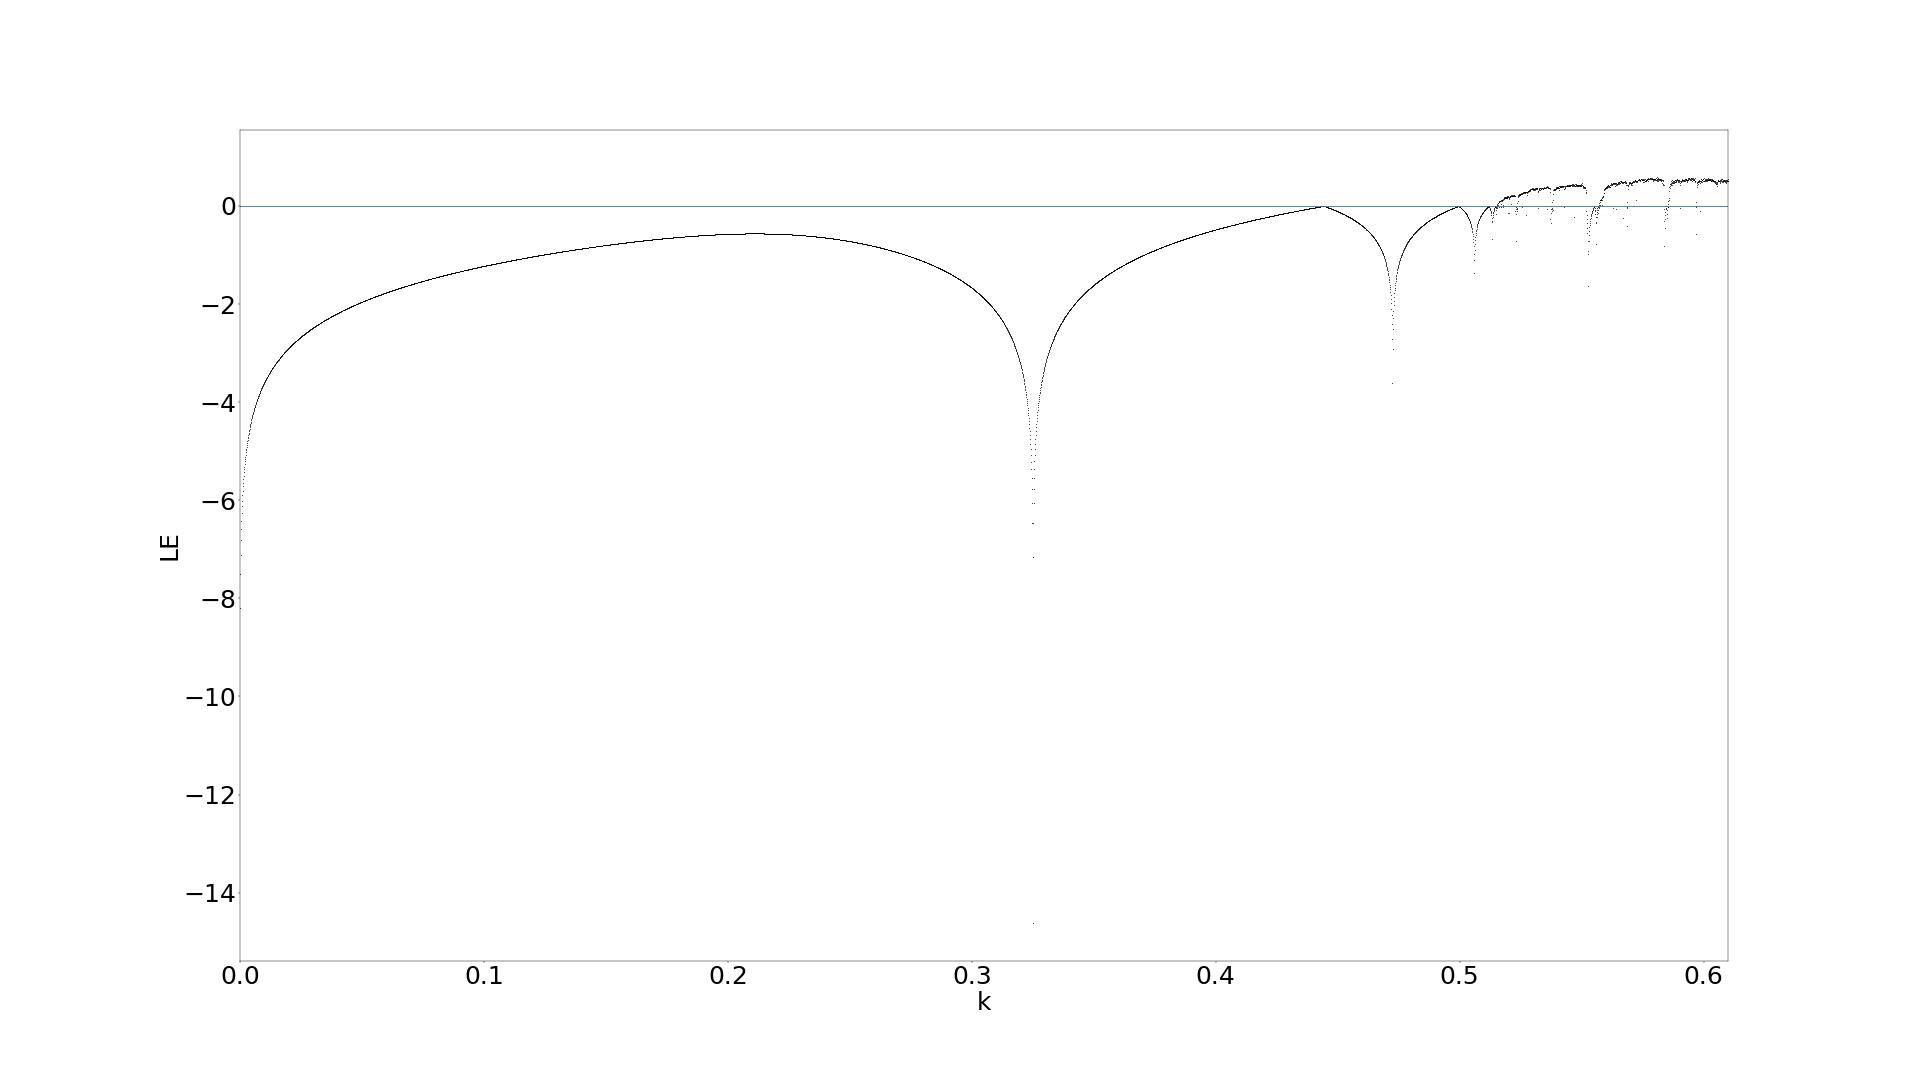
\includegraphics[width=0.6\linewidth]{LateX images/graphs q03/g2}
	\caption{ Διάγραμμα του εκθέτη Lyapunov σε συνάρτηση με την παράμετρο k, για a=1, b=2 και q=-0.3}
	\label{f:g9}
\end{figure}

\begin{figure}[h!]
	\centering
	\caption{Διαγράμματα της τιμής \(x_i\) με την τιμή \(x_{i+1}\) :}
	\begin{subfigure}[b]{0.25\textwidth}
		\centering
		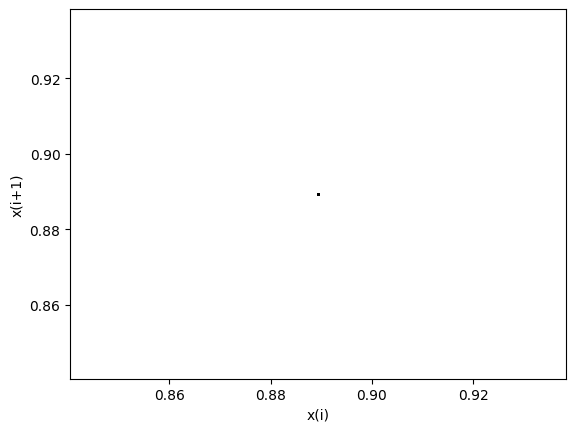
\includegraphics[width=\textwidth]{LateX images/graphs q03/g3}
		\caption{Για k=0.3}
		\label{f:k15}
	\end{subfigure}
	\hfill
	\begin{subfigure}[b]{0.25\textwidth}
		\centering
		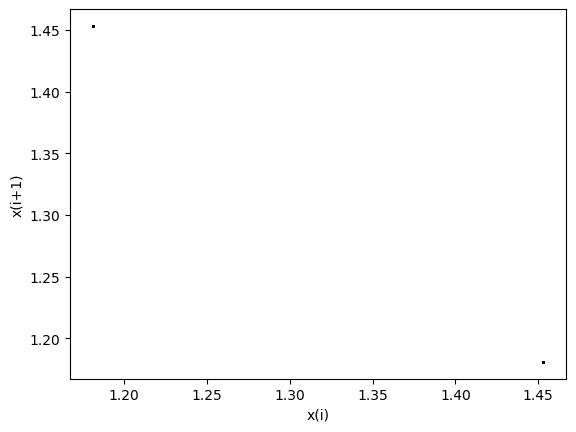
\includegraphics[width=\textwidth]{LateX images/graphs q03/g4}
		\caption{Για k=0.44}
		\label{f:k16}
	\end{subfigure}
	\hfill
	\begin{subfigure}[b]{0.25\textwidth}
		\centering
		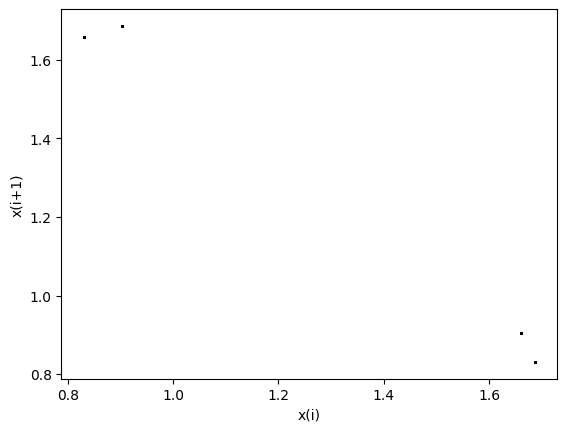
\includegraphics[width=\textwidth]{LateX images/graphs q03/g5}
		\caption{Για k=0.5}
		\label{f:k17}
	\end{subfigure}
	\hfill
	\begin{subfigure}[b]{0.25\textwidth}
		\centering
		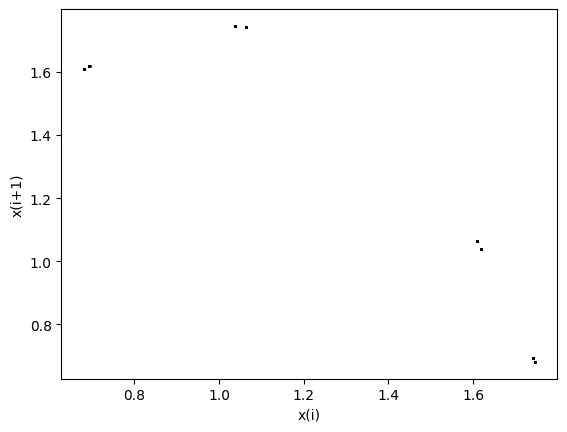
\includegraphics[width=\textwidth]{LateX images/graphs q03/g6}
		\caption{Για k=0.511}
		\label{f:k18}
	\end{subfigure}
	\hfill
	\begin{subfigure}[b]{0.25\textwidth}
		\centering
		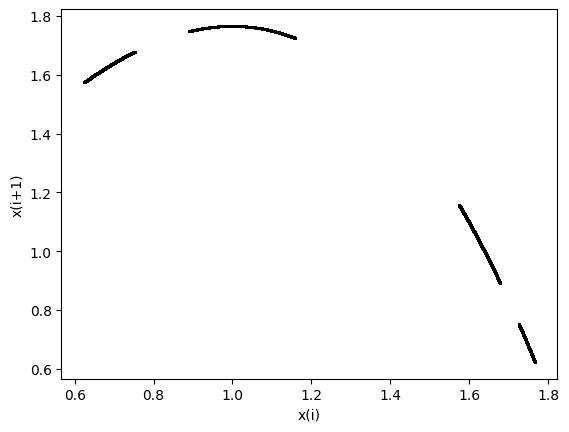
\includegraphics[width=\textwidth]{LateX images/graphs q03/g67}
		\caption{Για k=0.5165}
		\label{f:k19}
	\end{subfigure}
	\hfill
	\begin{subfigure}[b]{0.25\textwidth}
		\centering
		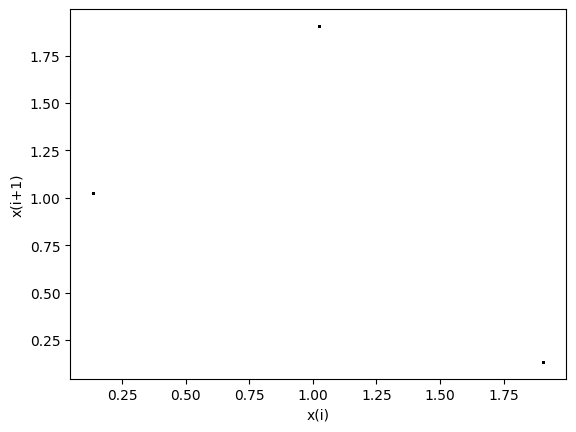
\includegraphics[width=\textwidth]{LateX images/graphs q03/g8}
		\caption{Για k=0.551}
		\label{f:k20}
	\end{subfigure}
	\hfill
	\begin{subfigure}[b]{0.25\textwidth}
		\centering
		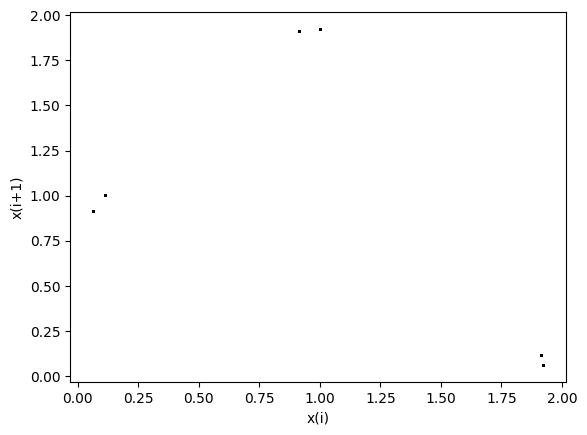
\includegraphics[width=\textwidth]{LateX images/graphs q03/g9}
		\caption{Για k=0.555}
		\label{f:k21}
	\end{subfigure}
	\hfill
	\begin{subfigure}[b]{0.25\textwidth}
		\centering
		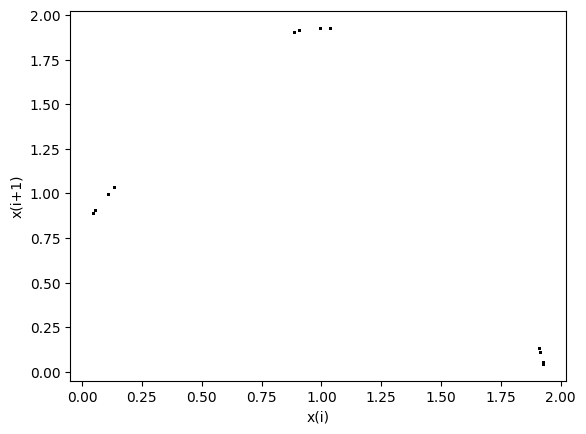
\includegraphics[width=\textwidth]{LateX images/graphs q03/g10}
		\caption{Για k=0.556}
		\label{f:k22}
	\end{subfigure}
	\hfill
	\begin{subfigure}[b]{0.25\textwidth}
		\centering
		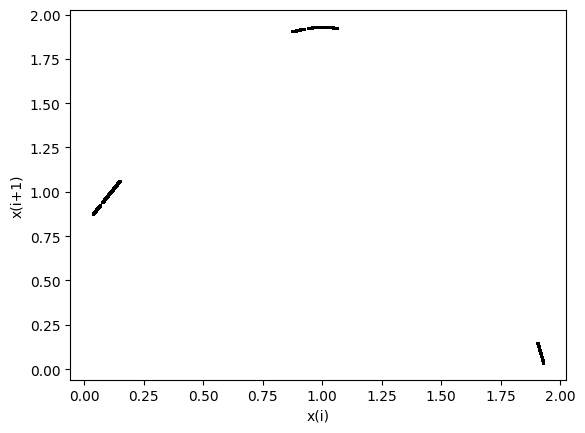
\includegraphics[width=\textwidth]{LateX images/graphs q03/g11}
		\caption{Για k=0.5573}
		\label{f:k23}
	\end{subfigure}
	\hfill
	\begin{subfigure}[b]{0.25\textwidth}
		\centering
		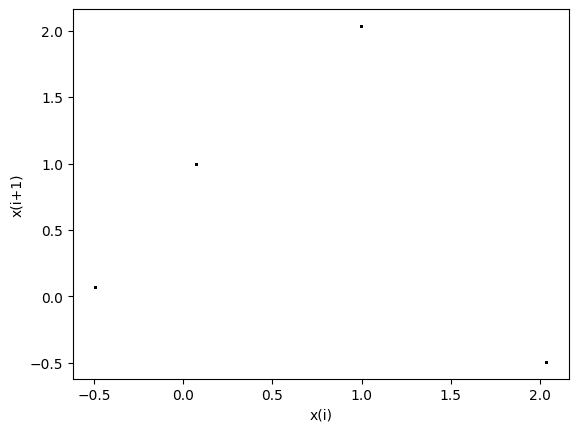
\includegraphics[width=\textwidth]{LateX images/graphs q03/g12}
		\caption{Για k=0.583}
		\label{f:k24}
	\end{subfigure}
	\hfill
	\begin{subfigure}[b]{0.25\textwidth}
		\centering
		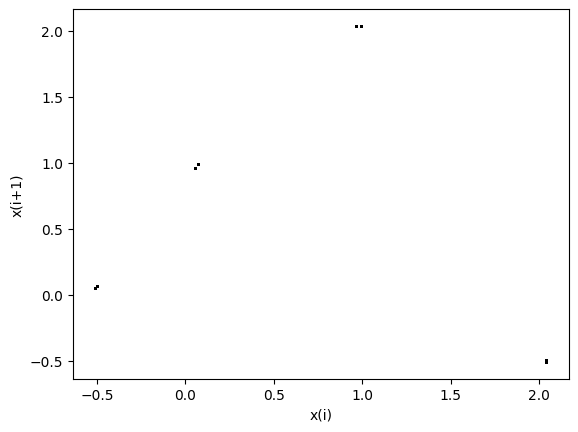
\includegraphics[width=\textwidth]{LateX images/graphs q03/g13}
		\caption{Για k=0.5846}
		\label{f:k25}
	\end{subfigure}
	\hfill
	\begin{subfigure}[b]{0.25\textwidth}
		\centering
		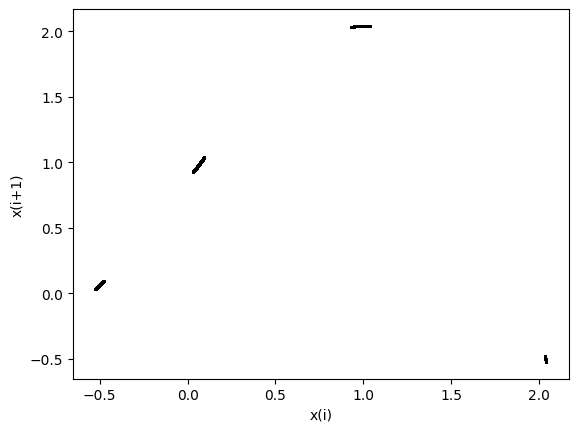
\includegraphics[width=\textwidth]{LateX images/graphs q03/g14}
		\caption{Για k=0.5851}
		\label{f:k26}
	\end{subfigure}
	
\end{figure}

\clearpage

\subsection{Για q=-0.5}

Στο σχήμα \ref{f:g10} παρατίθεται το διάγραμμα διακλάδωσης του συστήματος \ref{f:x1}, ως προς την παράμετρο k, για a=1, b=2 και q =- 0.5. Για αυτές τις τιμές των παραμέτρων το σύστημα ξεκινάει από περίοδο-1 για k = 0.3 , ενώ για  k = 0.48 εμφανίζει τον πρώτο διπλασιασμό της περιόδου. Τον δεύτερο διπλασιασμό τον εμφανίζει για k=0.53 (περίοδος-4) ,τον τρίτο για k=0.55 (περίοδος-8) και τον τέταρτο για k=0.5531 (περόδος-15).Στην συνέχεια για k>0.5534 το σύστημα εισέρχεται στο χάος , μέχρι να εξέλθει  για k=0.59(περίοδος-3) και να ξανά εισέλθει σε χάος μετά από δύο διπλασιασμούς k=0.59377 (περίοδος-6) ,για k>0.594.
Επομένως και σε αυτή την περίπτωση το σύστημα εισέρχεται στο χάος με διπλασιασμό της περιόδου. 
Επιπλέον, στο σχήμα \ref{f:g11} παρατίθεται το διάγραμμα των εκθετών Lyapunov για τιμές του k στο ίδιο διάστημα τιμών [0, 0.67].  Στο διάστημα τιμών   0<k<0.511 , στο 0.551<k<0.556, και στο 0.583<k<0.5846 παρατηρούμε ότι ο εκθέτης Lyapunov είναι συνεχώς αρνητικός, γεγονός που επιβεβαιώνει την περιοδική συμπεριφορά του συστήματος. Ενώ στα υπόλοιπα διαστήματα ο θετικός εκθέτης Lyapunov υποστηρίζει την χαοτική του συμπεριφορά, όπως έγινε φανερό και από το διάγραμμα διακλάδωσης.
Τέλος, στον Πίνακα \ref{tab:abc2} παρατίθενται ενδεικτικές τιμές της παραμέτρου k και η συμπεριφορά που παρουσιάζει το σύστημα για αυτές, σύμφωνα με το διάγραμμα διακλάδωσης, καθώς και τα αντίστοιχα σχήματα των διαγραμμάτων της τιμής \(x_i\) σε συνάρτηση με την τιμή \(x_{i+1}\). Από τα παραγόμενα σχήματα προκύπτει αριθμός σημείων αντίστοιχος με την περίοδο του συστήματος.

\begin{table}[h!]
	\centering
	\begin{tabular}{l | l | l}
		Παράμετρος k & Συμπεριφορά & Σχήμα\\
		\hline
		0.3 &  Περίοδος-1 & \ref{f:k1}\\
		0.48& Περίοδος-2 & \ref{f:k2}\\
		0.53& Περίοδος-4 & \ref{f:k2}\\
		0.55 &  Περίοδος-8 & \ref{f:k3}\\
		0.5531 & Περίοδος-15 & \ \\
		0.5534 & Χάος & \ref{f:k5}\\
		0.59 & Περίοδος-3 & \ref{f:k6})\\
		0.593 & Περίοδος-6 & \ref{f:k7}\\
		0.594 & Χάος & \ref{f:k9}\\
	\end{tabular}
	\caption{ Συμπεριφορά του υπό μελέτη συστήματος για διάφορες τιμές του k,για a=1, b=2 και q=-0.5}
	\label{tab:abc2}
\end{table}

\begin{figure}[h!]
	\centering
	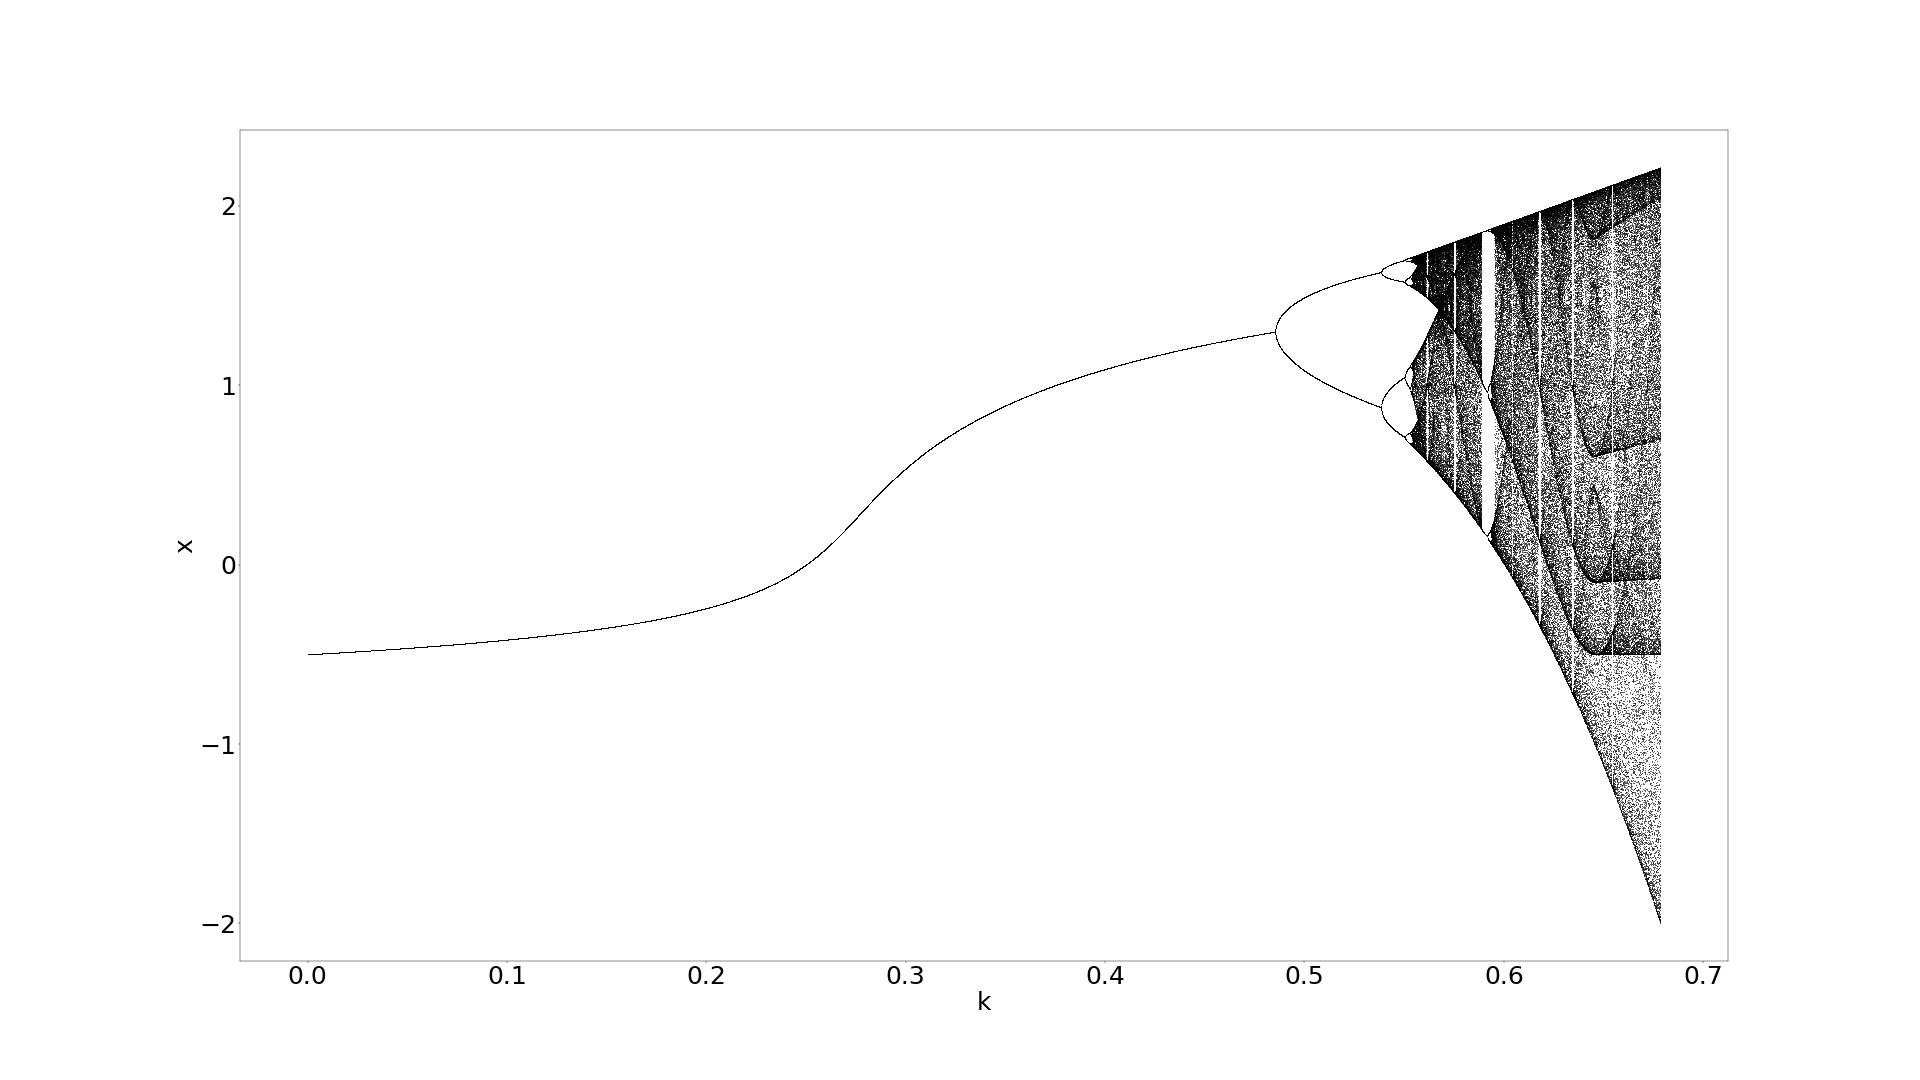
\includegraphics[width=0.6\linewidth]{LateX images/graphs q05/g1}
	\caption{ Διάγραμμα διακλάδωσης, για a=1, b=2 και q=-0.5}
	\label{f:g10}
\end{figure}

\begin{figure}[h!]
	\centering
	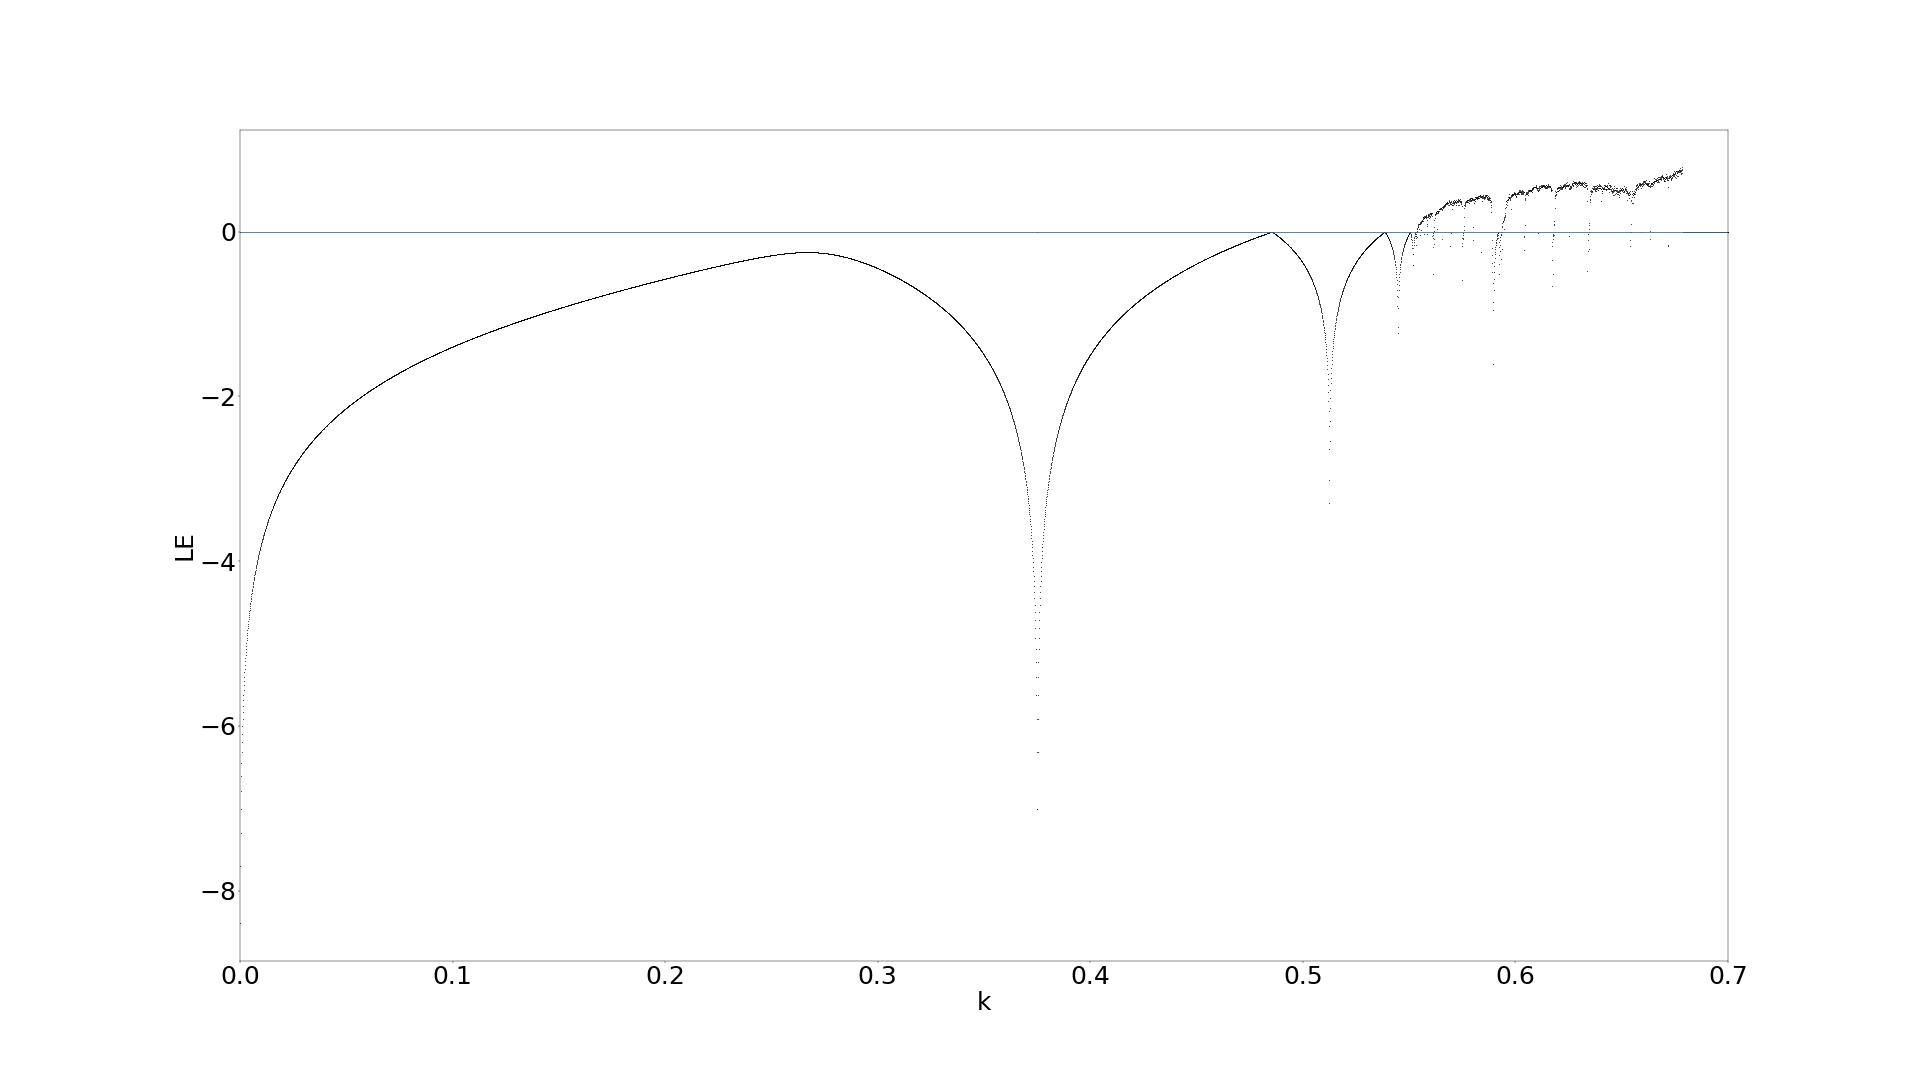
\includegraphics[width=0.6\linewidth]{LateX images/graphs q05/g2}
	\caption{ Διάγραμμα του εκθέτη Lyapunov σε συνάρτηση με την παράμετρο k, για a=1, b=2 και q=-0.5}
	\label{f:g11}
\end{figure}

\begin{figure}[h!]
	\centering
	\caption{Διαγράμματα της τιμής \(x_i\) με την τιμή \(x_{i+1}\) :}
	\begin{subfigure}[b]{0.25\textwidth}
		\centering
		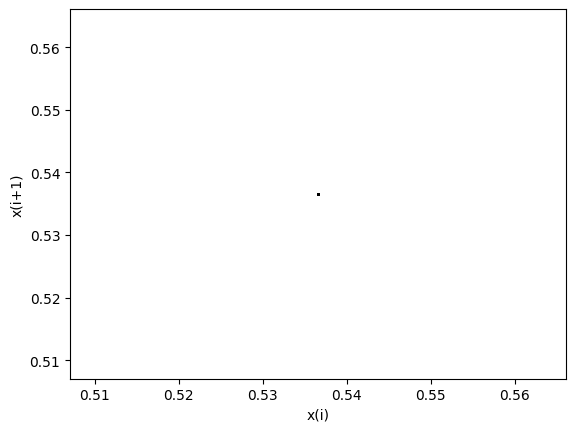
\includegraphics[width=\textwidth]{LateX images/graphs q05/g3}
		\caption{Για k=0.3}
		\label{f:k27}
	\end{subfigure}
	\hfill
	\begin{subfigure}[b]{0.25\textwidth}
		\centering
		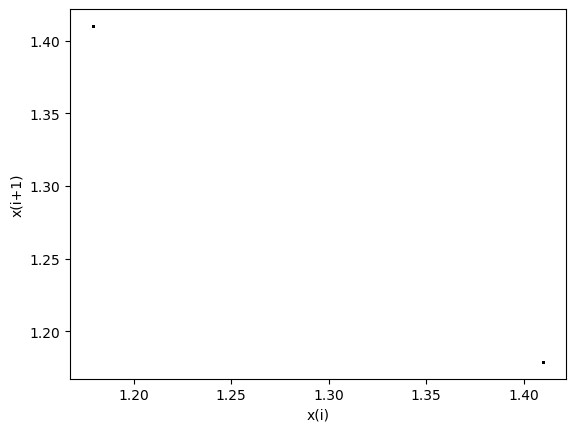
\includegraphics[width=\textwidth]{LateX images/graphs q05/g4}
		\caption{Για k=0.48}
		\label{f:k28}
	\end{subfigure}
	\hfill
	\begin{subfigure}[b]{0.25\textwidth}
		\centering
		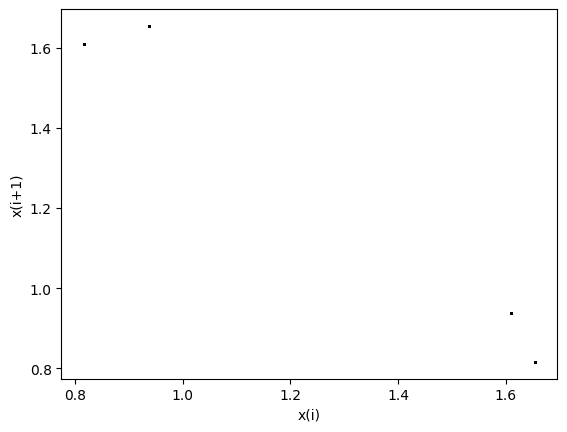
\includegraphics[width=\textwidth]{LateX images/graphs q05/g5}
		\caption{Για k=0.53}
		\label{f:k29}
	\end{subfigure}
	\begin{subfigure}[b]{0.25\textwidth}
		\centering
		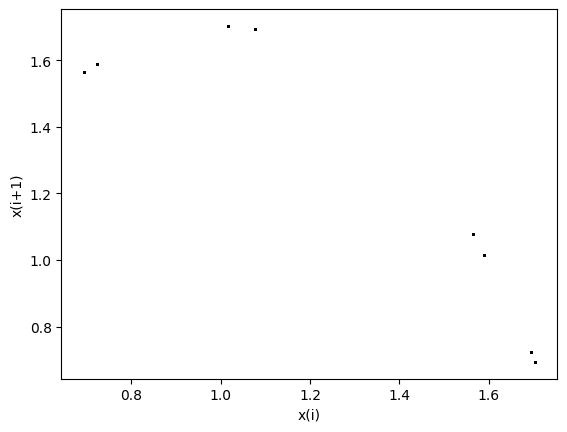
\includegraphics[width=\textwidth]{LateX images/graphs q05/g6}
		\caption{Για k=0.55}
		\label{f:k30}
	\end{subfigure}
	\hfill
	\begin{subfigure}[b]{0.25\textwidth}
		\centering
		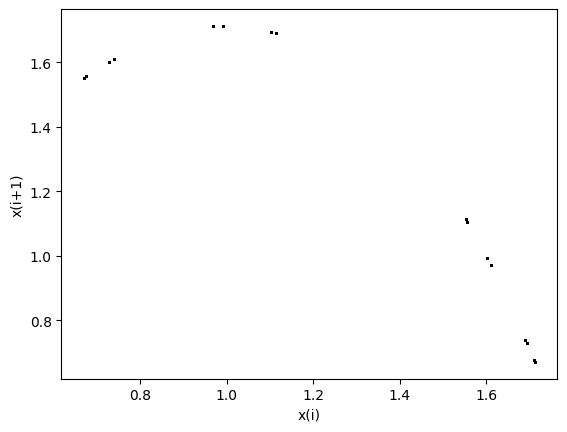
\includegraphics[width=\textwidth]{LateX images/graphs q05/g7}
		\caption{Για k=0.5531}
		\label{f:k31}
	\end{subfigure}
	\hfill
	\begin{subfigure}[b]{0.25\textwidth}
		\centering
		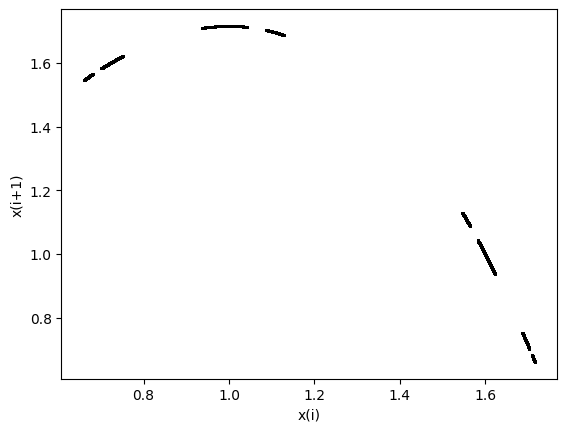
\includegraphics[width=\textwidth]{LateX images/graphs q05/g8}
		\caption{Για k=0.5534}
		\label{f:k32}
	\end{subfigure}
	\hfill
	\begin{subfigure}[b]{0.25\textwidth}
		\centering
		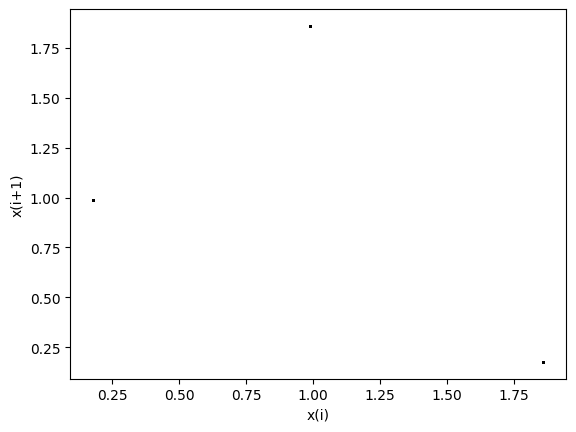
\includegraphics[width=\textwidth]{LateX images/graphs q05/g9}
		\caption{Για k=0.58}
		\label{f:k33}
	\end{subfigure}
	\hfill
	\begin{subfigure}[b]{0.25\textwidth}
		\centering
		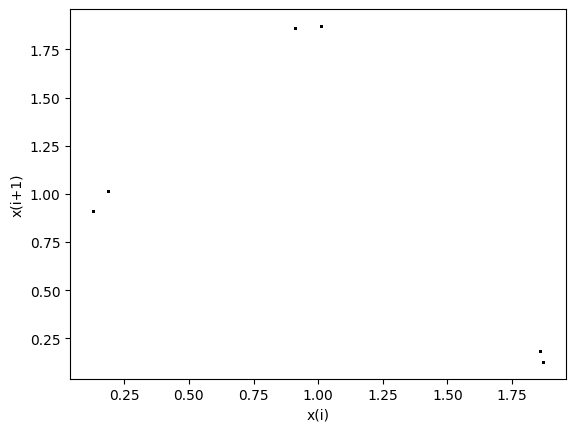
\includegraphics[width=\textwidth]{LateX images/graphs q05/g10}
		\caption{Για k=0.591}
		\label{f:k35}
	\end{subfigure}
	\hfill
	\begin{subfigure}[b]{0.25\textwidth}
		\centering
		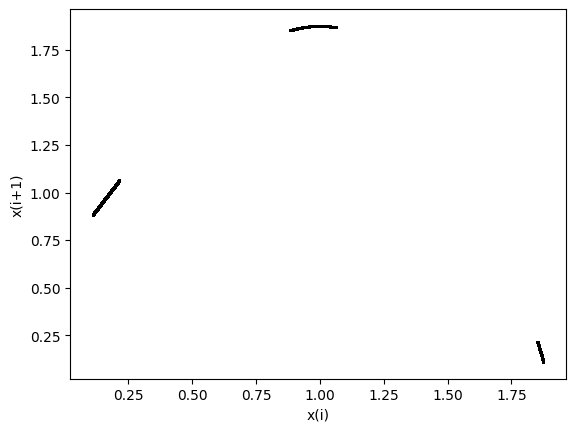
\includegraphics[width=\textwidth]{LateX images/graphs q05/g11}
		\caption{Για k=0.5927}
		\label{f:36}
	\end{subfigure}
		
\end{figure}

 \clearpage

\subsection{Για q=-0.7}

Στο σχήμα \ref{f:g12} παρατίθεται το διάγραμμα διακλάδωσης του συστήματος \ref{f:x1}, ως προς την παράμετρο k, για a=1, b=2 και q =- 0.7. Για αυτές τις τιμές των παραμέτρων το σύστημα ξεκινάει από περίοδο-1 για k = 0.3 αλλά από k[0.3469,0.3486] σπάει η περίοδος. Απο k=3.469 ξαναξεκινάει από περίοδο-1.Για  k = 0.52 εμφανίζει τον πρώτο διπλασιασμό της περιόδου. Τον δεύτερο διπλασιασμό τον εμφανίζει για k=0.57(περίοδος-4) ,τον τρίτο για k=0.592 (περίοδος-8) και τον τέταρτο για k=0.593(περόδος-15).Στην συνέχεια για k>0.593 το σύστημα εισέρχεται στο χάος , μέχρι να εξέλθει  για k=0.627(περίοδος-3) και να ξανά εισέλθει σε χάος μετά από δύο διπλασιασμούς k=0.63 (περίοδος-6)  k=0.631 (περίοδος-11),για k>0.631.
Επομένως και σε αυτή την περίπτωση το σύστημα εισέρχεται στο χάος με διπλασιασμό της περιόδου. 
Επιπλέον, στο σχήμα \ref{f:g11} παρατίθεται το διάγραμμα των εκθετών Lyapunov για τιμές του k στο ίδιο διάστημα τιμών [0, 0.72].  Στο διάστημα τιμών   0<k<0.594 , στο 0.627<k<0.632, παρατηρούμε ότι ο εκθέτης Lyapunov είναι συνεχώς αρνητικός, γεγονός που επιβεβαιώνει την περιοδική συμπεριφορά του συστήματος. Ενώ στα υπόλοιπα διαστήματα ο θετικός εκθέτης Lyapunov υποστηρίζει την χαοτική του συμπεριφορά, όπως έγινε φανερό και από το διάγραμμα διακλάδωσης.
Τέλος, στον Πίνακα \ref{tab:abc3} παρατίθενται ενδεικτικές τιμές της παραμέτρου k και η συμπεριφορά που παρουσιάζει το σύστημα για αυτές, σύμφωνα με το διάγραμμα διακλάδωσης, καθώς και τα αντίστοιχα σχήματα των διαγραμμάτων της τιμής \(x_i\) σε συνάρτηση με την τιμή \(x_{i+1}\). Από τα παραγόμενα σχήματα προκύπτει αριθμός σημείων αντίστοιχος με την περίοδο του συστήματος.

\begin{table}[h!]
	\centering
	\begin{tabular}{l | l | l}
		Παράμετρος k & Συμπεριφορά & Σχήμα\\
		\hline
		0.25 &  Περίοδος-1 & \ref{f:k37}\\
		0.3469&  Περίοδος-1 & \ref{f:k38}\\
		0.52& Περίοδος-2 & \ref{f:k39}\\
		0.57& Περίοδος-4 & \ref{f:k40}\\
		0.592 &  Περίοδος-8 & \ref{f:k41}\\
		0.593& Περίοδος-15 & \ref{f:k42}\\
		0.594 & Χάος & \ref{f:k43}\\
		0.627 & Περίοδος-3 & \ref{f:k44}\\
		0.630 & Περίοδος-6 & \ref{f:k45}\\
		0.631 & Περίοδος-11 & \ref{f:k46}\\
		0.632 & Χάος & \ref{f:k47}\\
	\end{tabular}
	\caption{ Συμπεριφορά του υπό μελέτη συστήματος για διάφορες τιμές του k,για a=1, b=2 και q=-0.7}
	\label{tab:abc3}
\end{table}

\begin{figure}[h!]
	\centering
	\includegraphics[width=0.6\linewidth]{LateX images/graphs q07/g1}
	\caption{ Διάγραμμα διακλάδωσης, για a=1, b=2 και q=-0.7}
	\label{f:g12}
\end{figure}
\begin{figure}[h!]
	\centering
	\includegraphics[width=0.6\linewidth]{"LateX images/graphs q07/g2 "}
	\caption{Διάγραμμα του εκθέτη Lyapunov σε συνάρτηση με την παράμετρο k, για a=1, b=2 και q=-0.7.}
	\label{f:g13}
\end{figure}

\begin{figure}[h!]
	\centering
	\caption{Διαγράμματα της τιμής \(x_i\) με την τιμή \(x_{i+1}\) :}
	\begin{subfigure}[b]{0.25\textwidth}
		\centering
		\includegraphics[width=\textwidth]{LateX images/graphs q07/g3}
		\caption{Για k=0.25}
		\label{f:k37}
	\end{subfigure}
	\hfill
	\begin{subfigure}[b]{0.25\textwidth}
		\centering
		\includegraphics[width=\textwidth]{LateX images/graphs q07/g4}
		\caption{Για k=0.3469}
		\label{f:k38}
	\end{subfigure}
	\hfill
	\begin{subfigure}[b]{0.25\textwidth}
		\centering
		\includegraphics[width=\textwidth]{LateX images/graphs q07/g5}
		\caption{Για k=0.52}
		\label{f:k39}
	\end{subfigure}
	\begin{subfigure}[b]{0.25\textwidth}
		\centering
		\includegraphics[width=\textwidth]{LateX images/graphs q07/g6}
		\caption{Για k=0.57}
		\label{f:k40}
	\end{subfigure}
	\hfill
	\begin{subfigure}[b]{0.25\textwidth}
		\centering
		\includegraphics[width=\textwidth]{LateX images/graphs q07/g7}
		\caption{Για k=0.592}
		\label{f:k41}
	\end{subfigure}
	\hfill
	\begin{subfigure}[b]{0.25\textwidth}
		\centering
		\includegraphics[width=\textwidth]{LateX images/graphs q07/g8}
		\caption{Για k=0.593}
		\label{f:k42}
	\end{subfigure}
	\hfill
	\begin{subfigure}[b]{0.25\textwidth}
		\centering
		\includegraphics[width=\textwidth]{LateX images/graphs q07/g9}
		\caption{Για k=0.594}
		\label{f:k43}
	\end{subfigure}
	\hfill
	\begin{subfigure}[b]{0.25\textwidth}
		\centering
		\includegraphics[width=\textwidth]{LateX images/graphs q07/g10}
		\caption{Για k=0.627}
		\label{f:k44}
	\end{subfigure}
	\hfill
	\begin{subfigure}[b]{0.25\textwidth}
		\centering
		\includegraphics[width=\textwidth]{LateX images/graphs q07/g11}
		\caption{Για k=0.63}
		\label{f:k45}
	\end{subfigure}
	\hfill
	\begin{subfigure}[b]{0.25\textwidth}
		\centering
		\includegraphics[width=\textwidth]{LateX images/graphs q07/g12}
		\caption{Για k=0.631}
		\label{f:k46}
	\end{subfigure}
	\hfill
	\begin{subfigure}[b]{0.25\textwidth}
	\centering
	\includegraphics[width=\textwidth]{LateX images/graphs q07/g13}
	\caption{Για k=0.632}
	\label{f:k47}
	\end{subfigure}
	
\end{figure}

\clearpage

\subsection{Για q=-0.9}

\begin{table}[h!]
	\centering
	\begin{tabular}{l | l | l}
		Παράμετρος k & Συμπεριφορά & Σχήμα\\
		\hline
		0.43 &  Περίοδος-1 & \ref{f:k48}\\
		0.436 &  Περίοδος-1 & \ref{f:k49}\\
		0.57& Περίοδος-2 & \ref{f:k50}\\
		0.62& Περίοδος-4 & \ref{f:k51}\\
		0.63 &  Περίοδος-8 & \ref{f:k52}\\
		0.633& Περίοδος-16 & \ref{f:k53}\\
		0.635& Χάος & \ref{f:k54}\\
		0.665 & Περίοδος-3 & \ref{f:k55}\\
		0.668 & Περίοδος-6 & \ref{f:k56}\\
		0.671 & Χάος & \ref{f:k57}\\
		0.72 & Περίοδος-1& \ref{f:k58}\\
	\end{tabular}
	\caption{ Συμπεριφορά του υπό μελέτη συστήματος για διάφορες τιμές του k,για a=1, b=2 και q=-0.9}
	\label{tab:abc4}
\end{table}

\begin{figure}[h!]
	\centering
	\includegraphics[width=0.6\linewidth]{LateX images/graphs q09/g1}
	\caption{ Διάγραμμα διακλάδωσης, για a=1, b=2 και q=-0.9}
	\label{f:g14}
\end{figure}

\begin{figure}[h!]
	\centering
	\includegraphics[width=0.6\linewidth]{LateX images/graphs q09/g2}
	\caption{Διάγραμμα του εκθέτη Lyapunov σε συνάρτηση με την παράμετρο k, για a=1, b=2 και q=-0.9}
	\label{f:g15}
\end{figure}

\begin{figure}[h!]
	\centering
	\caption{Διαγράμματα της τιμής \(x_i\) με την τιμή \(x_{i+1}\) :}
	\begin{subfigure}[b]{0.25\textwidth}
		\centering
		\includegraphics[width=\textwidth]{LateX images/graphs q09/g3}
		\caption{Για k=0.43}
		\label{f:k48}
	\end{subfigure}
	\hfill
	\begin{subfigure}[b]{0.25\textwidth}
		\centering
		\includegraphics[width=\textwidth]{LateX images/graphs q09/g4}
		\caption{Για k=0.436}
		\label{f:k49}
	\end{subfigure}
	\hfill
	\begin{subfigure}[b]{0.25\textwidth}
		\centering
		\includegraphics[width=\textwidth]{LateX images/graphs q09/g5}
		\caption{Για k=0.57}
		\label{f:k50}
	\end{subfigure}
	\begin{subfigure}[b]{0.25\textwidth}
		\centering
		\includegraphics[width=\textwidth]{LateX images/graphs q09/g6}
		\caption{Για k=0.62}
		\label{f:k51}
	\end{subfigure}
	\hfill
	\begin{subfigure}[b]{0.25\textwidth}
		\centering
		\includegraphics[width=\textwidth]{LateX images/graphs q09/g13}
		\caption{Για k=0.63}
		\label{f:k52}
	\end{subfigure}
	\hfill
	\begin{subfigure}[b]{0.25\textwidth}
		\centering
		\includegraphics[width=\textwidth]{LateX images/graphs q09/g7}
		\caption{Για k=0.633}
		\label{f:k53}
	\end{subfigure}
	\hfill
	\begin{subfigure}[b]{0.25\textwidth}
		\centering
		\includegraphics[width=\textwidth]{LateX images/graphs q09/g8}
		\caption{Για k=0.635}
		\label{f:k54}
	\end{subfigure}
	\hfill
	\begin{subfigure}[b]{0.25\textwidth}
		\centering
		\includegraphics[width=\textwidth]{LateX images/graphs q09/g9}
		\caption{Για k=0.665}
		\label{f:k55}
	\end{subfigure}
	\hfill
	\begin{subfigure}[b]{0.25\textwidth}
		\centering
		\includegraphics[width=\textwidth]{LateX images/graphs q09/g10}
		\caption{Για k=0.668}
		\label{f:k56}
	\end{subfigure}
	\hfill
	\begin{subfigure}[b]{0.25\textwidth}
		\centering
		\includegraphics[width=\textwidth]{LateX images/graphs q09/g11}
		\caption{Για k=0.671}
		\label{f:k57}
	\end{subfigure}
	\hfill
	\begin{subfigure}[b]{0.25\textwidth}
		\centering
		\includegraphics[width=\textwidth]{LateX images/graphs q09/g12}
		\caption{Για k=0.72}
		\label{f:k58}
	\end{subfigure}
	\hfill
	
\end{figure}

\clearpage

\subsection{Για q=-1.2}

\begin{table}[h!]
	\centering
	\begin{tabular}{l | l | l}
		Παράμετρος k & Συμπεριφορά & Σχήμα\\
		\hline
		0.55 &  Περίοδος-1 & \ref{f:k59}\\
		0.566 &  Περίοδος-1 & \ref{f:k60}\\
		0.63& Περίοδος-2 & \ref{f:k61}\\
		0.68& Περίοδος-4 & \ref{f:k62}\\
		0.69 &  Περίοδος-8 & \ref{f:k63}\\
		0.696& Χάος & \ref{f:k64}\\
		0.726& Περίοδος-3 & \ref{f:k65}\\
		0.729& Περίοδος-6 & \ref{f:k66}\\
		0.731& Χάος & \ref{f:k67}\\
		0.762 &  Περίοδος-1 & \ref{f:k68}\\
	\end{tabular}
	\caption{ Συμπεριφορά του υπό μελέτη συστήματος για διάφορες τιμές του k,για a=1, b=2 και q=-0.9}
	\label{tab:abc5}
\end{table}

\begin{figure}[h!]
	\centering
	\includegraphics[width=0.6\linewidth]{LateX images/graphs q12/g1}
	\caption{ Διάγραμμα διακλάδωσης, για a=1, b=2 και q=-1.2}
	\label{f:g16}
\end{figure}

\begin{figure}[h!]
	\centering
	\includegraphics[width=0.6\linewidth]{LateX images/graphs q12/g2}
	\caption{Διάγραμμα του εκθέτη Lyapunov σε συνάρτηση με την παράμετρο k, για a=1, b=2 και q=-1.2}
	\label{f:g17}
\end{figure}

\begin{figure}[h!]
	\centering
	\caption{Διαγράμματα της τιμής \(x_i\) με την τιμή \(x_{i+1}\) :}
	\begin{subfigure}[b]{0.25\textwidth}
		\centering
		\includegraphics[width=\textwidth]{LateX images/graphs q12/g3}
		\caption{Για k=0.55}
		\label{f:k59}
	\end{subfigure}
	\hfill
	\begin{subfigure}[b]{0.25\textwidth}
		\centering
		\includegraphics[width=\textwidth]{LateX images/graphs q12/g4}
		\caption{Για k=0.566}
		\label{f:k60}
	\end{subfigure}
	\hfill
	\begin{subfigure}[b]{0.25\textwidth}
		\centering
		\includegraphics[width=\textwidth]{LateX images/graphs q12/g5}
		\caption{Για k=0.63}
		\label{f:k61}
	\end{subfigure}
	\begin{subfigure}[b]{0.25\textwidth}
		\centering
		\includegraphics[width=\textwidth]{LateX images/graphs q12/g6}
		\caption{Για k=0.68}
		\label{f:k62}
	\end{subfigure}
	\hfill
	\begin{subfigure}[b]{0.25\textwidth}
		\centering
		\includegraphics[width=\textwidth]{LateX images/graphs q12/g7}
		\caption{Για k=0.69}
		\label{f:k63}
	\end{subfigure}
	\hfill
	\begin{subfigure}[b]{0.25\textwidth}
		\centering
		\includegraphics[width=\textwidth]{LateX images/graphs q12/g8}
		\caption{Για k=0.696}
		\label{f:k64}
	\end{subfigure}
	\hfill
	\begin{subfigure}[b]{0.25\textwidth}
		\centering
		\includegraphics[width=\textwidth]{LateX images/graphs q12/g9}
		\caption{Για k=0.726}
		\label{f:k65}
	\end{subfigure}
	\hfill
	\begin{subfigure}[b]{0.25\textwidth}
		\centering
		\includegraphics[width=\textwidth]{LateX images/graphs q12/g10}
		\caption{Για k=0.729}
		\label{f:k66}
	\end{subfigure}
	\hfill
	\begin{subfigure}[b]{0.25\textwidth}
		\centering
		\includegraphics[width=\textwidth]{LateX images/graphs q12/g11}
		\caption{Για k=0.731}
		\label{f:k67}
	\end{subfigure}
	\hfill
	\begin{subfigure}[b]{0.25\textwidth}
		\centering
		\includegraphics[width=\textwidth]{LateX images/graphs q12/g12}
		\caption{Για k=0.762}
		\label{f:k68}
	\end{subfigure}
	\hfill
	
\end{figure}

\clearpage

\subsection{Για q=-1.4}

\begin{table}[h!]
	\centering
	\begin{tabular}{l | l | l}
		Παράμετρος k & Συμπεριφορά & Σχήμα\\
		\hline
		0.5 &  Περίοδος-1 & \ref{f:k59}\\
		0.54 &  Περίοδος-2 & \ref{f:k60}\\
		0.65& Περίοδος-1 & \ref{f:k61}\\
		0.68& Περίοδος-2 & \ref{f:k62}\\
		0.725 &  Περίοδος-4 & \ref{f:k63}\\
		0.735& Περίοδος-8 & \ref{f:k64}\\
		0.737& Περίοδος-15 & \ref{f:k65}\\
		0.738& Χάος & \ref{f:k66}\\
		0.767 &  Περίοδος-3& \ref{f:k68}\\
		0.769 &  Περίοδος-6& \ref{f:k68}\\
		0.77 &  Χάος& \ref{f:k68}\\
		0.8 &  Περίοδος-2& \ref{f:k68}\\
		
	\end{tabular}
	\caption{ Συμπεριφορά του υπό μελέτη συστήματος για διάφορες τιμές του k,για a=1, b=2 και q=-0.9}
	\label{tab:abc6}
\end{table}

[0,0.91]

	\null
	\thispagestyle{empty}
	\newpage
	\chapter{Παραλλαγή του sine-sinh Χάρτη}
	Στο κεφάλαιο αυτό παρουσιάζεται αναλυτικά η μελέτη της δυναμικής συμπεριφοράς ενός διακριτού συστήματος που αποτελεί παραλλαγή του γνωστού \emph{sine-sinh-sine} Χάρτη. Για επιλεγμένες τιμές της παραμέτρου του μπορεί να παρουσιάσει χαοτική συμπεριφορά όπως και φαινόμενα που σχετίζονται με τη μη-γραμμική δυναμική. Για τη μελέτη χρησιμοποιήθηκαν τα διαγράμματα διακλάδωσης, οι εκθέτες Lyapunov και οι απεικονίσεις της τιμής \(x_i\) σε συνάρτηση με  την τιμή \(x_{i+1}\).

Ο \emph{sine-sinh-sine} Χάρτης που αποτέλεσε τη βάση του προτεινόμενου σε αυτή την ενότητα, χάρτη, περιγράφεται από την παρακάτω εξίσωση \cite{b10}:

\begin{equation}
	x_{i+1}=k*\sin(\pi*\sinh(\pi*\sin(\pi* x_i)))
	\label{f:x2}
\end{equation}


Στην εξίσωση (\ref{f:x2})αντικαταστάθηκε η παράμετρος $\pi$
με την παράμετρο k, ένα σταθερό όρο q και έναν ακέραιο αριθμό. Έτσι προέκυψε η προτεινόμενη παραλλαγή του Λογιστικού Χάρτη,

\begin{equation}
	x_{i+1}=k*\sin(k*\sinh(q*\sin(2 * x_i)))
	\label{f:x3}
\end{equation}
όπου k, q παράμετροι.\\

Για την εύρεση της δυναμικής συμπεριφοράς του συστήματος (3.2) εξετάστηκε μια περιοχή τιμών των συγκεκριμένων παραμέτρων. Πιο συγκεκριμένα, στη μελέτη που πραγματοποιήθηκε η αρχική συνθήκη του συστήματος ($x_0 =0.1$) παρέμεινε  σταθερή, ενώ η τιμή της παραμέτρου q μεταβαλλόταν στο διάστημα $[-0.3,-0.5]$ με βήμα $0.2$. Έτσι, για κάθε περίπτωση παράχθηκαν το διάγραμμα διακλάδωσης, το διάγραμμα των εκθετών Lyapunov και το διάγραμμα της τιμής \(x_i\) σε συνάρτηση με  την τιμή \(x_{i+1}\), τα οποία παρουσιάζονται και αναλύονται στη συνέχεια.\\


\vspace{\fill}

\section{Για \emph{q} = -0.3}


Στo Σχ. \ref{f:g44} παρατίθεται τα διάγραμμα διακλάδωσης του συστήματος (\ref{f:x3}), ως προς την παράμετρο k, για $q =- 0.3$. 
Στον πίνακα \ref{tab:abc10} φαίνεται η πορεία του συστήματος και για ποιες τιμές της παραμέτρου k το σύστημα εμφανίζει περιοδική ή χαοτική συμπεριφορά, σύμφωνα με το διάγραμμα διακλάδωσης του Σχ. \ref{f:g44}. Επίσης παρατηρείται συνοριακή κρίση ελκυστών για διάφορες τιμές του k (2.27, 2.31, 2.43, 2.671, 2.76, 2.935, 3.293, 3.48, 3.629, 3.79), το οποίο φαίνεται ξεκάθαρα στο διάγραμμα διακλάδωσης του Σχ. \ref{f:g44}, στην μεταπήδηση του συστήματος από χαοτική συμπεριφορά σε \emph{περίοδο - 1} και \emph{περίοδο - 2}. Οι αντίστοιχες τιμές του k για αυτά τα σημεία του διαγράμματος υπάρχουν στο Πίνακα \ref{tab:abc10}, όπως και τα αντίστοιχα διαγράμματα της τιμής \(x_i\) σε συνάρτηση με την τιμή \(x_{i+1}\) του Σχ. \ref{f:k246}. Από τα παραγόμενα σχήματα προκύπτει αριθμός σημείων αντίστοιχος με την περίοδο του συστήματος.

Τέλος, στο Σχ. \ref{f:g45} παρατίθεται το διάγραμμα των εκθετών Lyapunov για τιμές του k στο ίδιο διάστημα τιμών $[0, 4.2]$. Οι τιμές του Πίνακα \ref{tab:abc10} που έχουν περιοδική συμπεριφορά αντιστοιχούν σε τιμές του διαγράμματος του Σχ. \ref{f:g44}, όπου o εκθέτης Lyapunov είναι συνεχώς αρνητικός, γεγονός που επιβεβαιώνει την συμπεριφορά του. Ενώ για τις υπόλοιπες τιμές ο θετικός εκθέτης Lyapunov υποστηρίζει τη χαοτική του συμπεριφορά, όπως γίνεται φανερό και από το διάγραμμα διακλάδωσης.\\\\

\begin{figure}[ht]
	\centering
	\includegraphics[width=1\linewidth]{LateX images/sine q=-0.3/g1}
	\caption{Διάγραμμα διακλάδωσης, για $q=-0.3$.}
	\label{f:g44}
\end{figure}



\begin{table}[ht]
	\centering
	\caption{ Συμπεριφορά του υπό μελέτη συστήματος για διάφορες τιμές του k, για $q=-0.3$ }
	\label{tab:abc10}
	\begin{tabular}{l | l}
		Παράμετρος k & Συμπεριφορά \\
		\hline
		0.25 &  Περίοδος -  1 \\
		1.287 &  Περίοδος -  2 \\
		2.17& Περίοδος -  4 \\
		2.2& Περίοδος -  8 \\
		2.21 & Xάος \\
		2.27& Περίοδος - 10 \\
		2.272& Χάος \\
		2.31& Περίοδος - 6 \\
		2.32 &  Χάος \\
		2.43 &  Περίοδος -  3 \\
		2.435 &  Χάος \\
		2.671 &  Περίοδος -  3\\
		2.672 & Περίοδος - 6\\
		2.675 & Χάος\\
		2.76 &Περίοδος - 6 \\
		2.77& Χάος\\
		2.935 & Περίοδος -  1\\
		3.14& Περίοδος - 2\\
		3.22 & Περίοδος -  4\\
		3.79 &Περίοδος - 4\\
		3.8 & Χάος\\
		4.09& Περίοδος - 2
		
	\end{tabular}
	
\end{table}


\begin{figure}[ht]
	\centering
	\includegraphics[width=1\linewidth]{LateX images/sine q=-0.3/g2}
	\caption{Διάγραμμα των εκθετών Lyapunov σε συνάρτηση με την παράμετρο k, για $q=-0.3$.}
	\label{f:g45}
\end{figure}



\begin{figure}[ht]
	\centering
	\begin{subfigure}[b]{0.4\textwidth}
		\centering
		\includegraphics[width=\textwidth]{LateX images/sine q=-0.3/g3}
		\caption{Για $k=2.27$}
		\label{f:k116}
	\end{subfigure}
	\hfill
	\begin{subfigure}[b]{0.4\textwidth}
		\centering
		\includegraphics[width=\textwidth]{LateX images/sine q=-0.3/g4}
		\caption{Για $k=2.31$}
		\label{f:k117}
	\end{subfigure}
	\hfill
	\begin{subfigure}[b]{0.4\textwidth}
		\centering
		\includegraphics[width=\textwidth]{LateX images/sine q=-0.3/g5}
		\caption{Για $k=2.43$}
		\label{f:k118}
	\end{subfigure}
	\hfill
	\begin{subfigure}[b]{0.4\textwidth}
		\centering
		\includegraphics[width=\textwidth]{LateX images/sine q=-0.3/g6}
		\caption{Για $k=2.671$}
		\label{f:k119}
	\end{subfigure}
	\hfill
	\begin{subfigure}[b]{0.4\textwidth}
		\centering
		\includegraphics[width=\textwidth]{LateX images/sine q=-0.3/g7}
		\caption{Για $k=2.76$}
		\label{f:k120}
	\end{subfigure}
	\hfill
	\begin{subfigure}[b]{0.4\textwidth}
		\centering
		\includegraphics[width=\textwidth]{LateX images/sine q=-0.3/g20}
		\caption{Για $k=3.8$}
		\label{f:k126}
	\end{subfigure}
	\hfill		
	\caption{Διαγράμματα της τιμής \(x_i\) σε συνάρτηση με την τιμή \(x_{i+1}\).}
	\label{f:k246}
\end{figure}

\clearpage 
\section{Για \emph{q} = -0.5}

Στο Σχ. \ref{f:48} παρατίθενται τα διαγράμματα διακλάδωσης του συστήματος \ref{f:x3}, ως προς την παράμετρο k, για $q =-0.5$ και για διαφορετικές αρχικές συνθήκες, δηλαδή για διαφορετικό \(x_0\). Συγκρίνοντας το διάγραμμα του Σχ. \ref{f:g46} (\(x_0=0.1\)) με τα υπόλοιπα διαγράμματα διακλάδωσης των Σχ. \ref{f:g47} (\(x_0=0.5\)), \ref{f:g48} (\(x_0=1\)), παρατηρείται ότι για $q=-0.5$ εμφανίζεται το φαινόμενο της συνύπαρξης ελκυστών. Η συμπεριφορά του συστήματος για τις διάφορες περιπτώσεις επιβεβαιώνεται και από τα αντίστοιχα διαγράμματα Lyapunov των Σχ. (\ref{f:g49}, \ref{f:g50}, \ref{f:g51}), όπως και απο το διάγραμμα διακλάδωσης του Σχ. \ref{f:g54}, όπου η κάθε αρχική συνθήκη εμφανίζεται με διαφορετικό χρώμα.

Στον Πίνακα \ref{tab:abc11} φαίνεται η πορεία του συστήματος και για ποιες τιμές της παραμέτρου k το σύστημα εμφανίζει περιοδική ή χαοτική συμπεριφορά, σύμφωνα με το διάγραμμα διακλάδωσης του Σχ. \ref{f:g46}. Οι τιμές αυτές αντιστοιχούν στα σχήματα των διαγραμμάτων της τιμής \(x_i\) σε συνάρτηση με την τιμή \(x_{i+1}\). Από τα παραγόμενα Σχ. \ref{f:g58} προκύπτει αριθμός σημείων αντίστοιχος με την περίοδο του συστήματος.

Επίσης παρατηρείται η συνοριακή κρίση ελκυστών για διάφορες τιμές του k (1.773, 1.8, 1.831, 1.93, 2.03, 2.141, 2.2, 2.38,
2.88, 2.99, 3.04, 3.2, 3.35, 3.4, 3.44, 3.62, 3.93), όπως και το φαινόμενο της υστέρησης το οποίο διακρίνεται στα κενά που δημιουργούνται στις σκιαγραφημένες περιοχές 1 και 2. Οι αντίστοιχες τιμές του k για αυτά τα σημεία του διαγράμματος υπάρχουν στο Πίνακα \ref{tab:abc11}.

Επιπλέον παρατηρούμε στα διαγράμματα των Σχ. \ref{f:g237}, \ref{f:g238}, \ref{f:g239} το φαινόμενο της αντιμονοτονικότητας. Συγκεκριμένα στα διαγράμματα του Σχ. \ref{f:g237} εμφανίζεται μία χαοτική φυσαλίδα (το σύστημα εισέρχεται στο χάος με διπλασιασμό της περιόδου και στη συνέχεια εξέρχεται από αυτό με ανάστροφη ακολουθία διπλασιασμού της περιόδου), για $k=3.85$, της οποίας η εξέλιξη φαίνεται στα υπόλοιπα δύο διαγράμματα των. Σχ. \ref{f:g238}, \ref{f:g239}, όπου για διαφορετικές αρχικές συνθήκες $x_0$ διακρίνεται καλύτερα.
Μεταξύ αυτών των χαοτικών φυσαλίδων παρατηρούμε και τις δύο περιπτώσεις του φαινομένου, δηλαδή τον ορθό και τον ανάστροφο διπλασιασμό της περιόδου. Στα Σχ. \ref{f:g238}, \ref{f:g239} παρατηρείται ότι για $k=3.95$ ξεκινάει η ανάστροφη φυσαλίδα με \emph{περίοδο-1}.

Τέλος, στο σχήμα \ref{f:g49} παρατίθεται το διάγραμμα των εκθετών Lyapunov για τιμές του k στο ίδιο διάστημα τιμών $[0, 4.2]$. Οι τιμές του Πίνακα \ref{tab:abc11} που έχουν περιοδική συμπεριφορά αντιστοιχούν σε τιμές του διαγράμματος του Σχ. \ref{f:g49}, όπου ο εκθέτης Lyapunov είναι συνεχώς αρνητικός, γεγονός που επιβεβαιώνει την συμπεριφορά τους. Ενώ για τις υπόλοιπες τιμές ο θετικός εκθέτης Lyapunov υποστηρίζει την χαοτική τους συμπεριφορά, όπως γίνεται φανερό και από το διάγραμμα διακλάδωσης.





\begin{table}[ht]
	\centering
	\caption{ Συμπεριφορά του υπό μελέτη συστήματος για διάφορες τιμές του k, για $q=-0.5$ }
	\label{tab:abc11}
	\begin{tabular}{l | l}
		Παράμετρος k & Συμπεριφορά \\
		\hline
		0.25 &  Περίοδος -  1 \\
		1 &  Περίοδος -  2 \\
		1.7& Περίοδος -  4 \\
		1.748& Περίοδος -  8 \\
		1.75 & Xάος \\
		1.773& Περίοδος - 6 \\
		1.774& Περίοδος - 12\\
		1.775& Χάος \\
		1.8& Περίοδος - 10 \\
		1.806 &  Χάος \\
		2.03 &  Περίοδος -  4\\
		2.06 &Χάος \\
		2.88& Περίοδος -  3\\
		2.89 & Χάος\\
		2.99 &  Περίοδος -  6\\
		3 &  Περίοδος - 12\\
		3.01 &  Χάος\\
		3.04 & Περίοδος - 4\\
		3.08 & Χάος\\
		3.2 & Περίοδος -2\\
		3.206 & Περίοδος -  4\\
		3.23 & Περίοδος -  2\\
		3.24 & Χάος\\
		3.35 & Περίοδος -  4\\
		3.36 & Χάος\\
		3.4 & Περίοδος -  4\\
		3.41 & Χάος\\
		3.44 & Περίοδος -  4\\
		3.45 & Χάος\\
		3.62 & Περίοδος -  2\\
		3.8 & Περίοδος -  4\\
		3.84 & Χάος\\
		3.94 & Περίοδος -  8\\
		3.95 & Περίοδος -  4\\
		3.96 & Περίοδος -  8\\
		3.97 & Περίοδος -  16\\
		3.98 & Χάος\\
		4 & Περίοδος -  6\\
		4.05&Περίοδος - 4\\
		4.07 & Χάος\\
		
	\end{tabular}
	
\end{table}


\begin{figure}[ht]
	\centering
	\begin{subfigure}[b]{0.8\textwidth}
		\centering
		\includegraphics[width=\textwidth]{LateX images/sine q=-0.5/g4}
		\caption{\(x_0=0.1\)}
		\label{f:g46}
	\end{subfigure}
	\hfill
	\begin{subfigure}[b]{0.8\textwidth}
		\centering
		\includegraphics[width=\textwidth]{LateX images/sine q=-0.5/g5}
		\caption{\(x_0=0.5\)}
		\label{f:g47}
	\end{subfigure}
	\hfill
	\begin{subfigure}[b]{0.8\textwidth}
		\centering
		\includegraphics[width=\textwidth]{LateX images/sine q=-0.5/g6}
		\caption{\(x_0=1\)}
		\label{f:g48}
	\end{subfigure}
	\caption{ Διαγράμματα διακλάδωσης, για $q=-0.5$}
	\label{f:48}
\end{figure}

\begin{figure}[ht]
	\centering
	
	\begin{subfigure}[b]{0.8\textwidth}
		\centering
		\includegraphics[width=\textwidth]{LateX images/sine q=-0.5/g8}
		\caption{Για \(x_0=0.1\)}
		\label{f:g49}
	\end{subfigure}
	\hfill
	\begin{subfigure}[b]{0.8\textwidth}
		\centering
		\includegraphics[width=\textwidth]{LateX images/sine q=-0.5/g9}
		\caption{Για \(x_0=0.5\)}
		\label{f:g50}
	\end{subfigure}
	\hfill
	\begin{subfigure}[b]{0.8\textwidth}
		\centering
		\includegraphics[width=\textwidth]{LateX images/sine q=-0.5/g10}
		\caption{Για \(x_0=1\)}
		\label{f:g51}
	\end{subfigure}
	\hfill
	\caption{ Διαγράμματα των εκθετών Lyapunov σε συνάρτηση με την παράμετρο k, για $q=-0.5$.}
	\label{f:g236}
\end{figure}



\begin{figure}[ht]
	\centering
	
	\begin{subfigure}[b]{0.8\textwidth}
		\centering
		\includegraphics[width=\textwidth]{LateX images/sine q=-0.5/g3}
		\caption{Περιοχή 1 (βλ. Σχ. \ref{f:g46})}
		\label{f:g52}
	\end{subfigure}
	\hfill
	\begin{subfigure}[b]{0.8\textwidth}
		\centering
		\includegraphics[width=\textwidth]{LateX images/sine q=-0.5/g3.2}
		\caption{Περιοχή 2 (βλ. Σχ. \ref{f:g46})}
		\label{f:g533}
	\end{subfigure}
	
	\caption{Διαγράμματα διακλάδωσης για διάφορες τιμές του $x_0=0.1$. }
	\label{f:g237}
\end{figure}
\begin{figure}[ht]
	\centering	
	\begin{subfigure}[b]{0.8\textwidth}
		\centering
		\includegraphics[width=\textwidth]{LateX images/sine q=-0.5/g7}
		\caption{Περιοχή 1 (βλ. Σχ. \ref{f:g47})}
		\label{f:g522}
	\end{subfigure}
	\hfill
	\begin{subfigure}[b]{0.8\textwidth}
		\centering
		\includegraphics[width=\textwidth]{LateX images/sine q=-0.5/g7.2}
		\caption{Περιοχή 2 βλ. Σχ. \ref{f:g47})}
		\label{f:g523}
	\end{subfigure}
	\caption{Διαγράμματα διακλάδωσης για διάφορες τιμές του $x_0=0.5$. }
	\label{f:g238}
\end{figure}
\begin{figure}[ht]
	\centering
	
	\begin{subfigure}[b]{0.8\textwidth}
		\centering
		\includegraphics[width=\textwidth]{LateX images/sine q=-0.5/g12}
		\caption{Περιοχή 1 (βλ. Σχ. \ref{f:g48})}
		\label{f:g524}
	\end{subfigure}
	\hfill
	\begin{subfigure}[b]{0.8\textwidth}
		\centering
		\includegraphics[width=\textwidth]{LateX images/sine q=-0.5/g12.2}
		\caption{Περιοχή 2 (βλ. Σχ. \ref{f:g48})}
		\label{f:g525}
	\end{subfigure}
	\caption{Διαγράμματα διακλάδωσης για διάφορες τιμές του $x_0=1$. }
	\label{f:g239}
\end{figure}

\begin{figure}[ht]
	\centering
	
	\begin{subfigure}[b]{0.8\textwidth}
		\centering
		\includegraphics[width=\textwidth]{LateX images/sine q=-0.5/g2}
		\caption{$x_0=0.1$}
		\label{f:g54}
	\end{subfigure}
	\hfill
	\begin{subfigure}[b]{0.8\textwidth}
		\centering
		\includegraphics[width=\textwidth]{LateX images/sine q=-0.5/g14}
		\caption{$x_0=0.5$}
		\label{f:g55}
	\end{subfigure}
	\begin{subfigure}[b]{0.8\textwidth}
		\centering
		\includegraphics[width=\textwidth]{LateX images/sine q=-0.5/g15}
		\caption{$x_0=1$}
		\label{f:g56}
	\end{subfigure}
	
	\caption{Διαγράμματα διακλάδωσης για διάφορες τιμές του $x_0$. }
\end{figure}

\begin{figure}[ht]
	\centering
	\includegraphics[width=1\linewidth]{LateX images/sine q=-0.5/g11}
	\caption{Διάγραμμα διακλάδωσης, για όλες τις διαφορετικές αρχικές συνθήκες $x_0$.}
	\label{f:g57}
\end{figure}

\begin{figure}[ht]
	\centering
	\begin{subfigure}[b]{0.4\textwidth}
		\centering
		\includegraphics[width=\textwidth]{LateX images/sine q=-0.5/g16}
		\caption{Για $k=1.775$}
		\label{f:k127}
	\end{subfigure}
	\hfill
	\begin{subfigure}[b]{0.4\textwidth}
		\centering
		\includegraphics[width=\textwidth]{LateX images/sine q=-0.5/g17}
		\caption{Για $k=2.03$}
		\label{f:k128}
	\end{subfigure}
	\hfill
	\begin{subfigure}[b]{0.4\textwidth}
		\centering
		\includegraphics[width=\textwidth]{LateX images/sine q=-0.5/g19}
		\caption{Για $k=2.84$}
		\label{f:k129}
	\end{subfigure}
	\hfill
	\begin{subfigure}[b]{0.4\textwidth}
		\centering
		\includegraphics[width=\textwidth]{LateX images/sine q=-0.5/g18}
		\caption{Για $k=3$}
		\label{f:k130}
	\end{subfigure}
	\hfill
	\begin{subfigure}[b]{0.4\textwidth}
		\centering
		\includegraphics[width=\textwidth]{LateX images/sine q=-0.5/g20}
		\caption{Για $k=3.01$}
		\label{f:k131}
	\end{subfigure}
	\hfill
	\begin{subfigure}[b]{0.4\textwidth}
		\centering
		\includegraphics[width=\textwidth]{LateX images/sine q=-0.5/g21}
		\caption{Για $k=4$}
		\label{f:k132}
	\end{subfigure}
	\hfill			
	\caption{Διαγράμματα της τιμής \(x_i\) σε συνάρτηση με την τιμή \(x_{i+1}\).}
	\label{f:g58}
\end{figure}

\clearpage

\section{Συμπεράσματα}

Σε αυτό το κεφάλαιο παρουσιάστηκε μία παραλλαγή του \emph{sine-sinh-sine} Χάρτη, της οποίας βασικό χαρακτηριστικό είναι η χαοτική συμπεριφορά που καταγράφηκε σε όλες τις περιπτώσεις που ελέγχθηκαν για την παράμετρο q, όπως και για τα επί μέρους φαινόμενα που οδηγούν σε αυτήν.

Ειδικότερα, το συνηθέστερο φαινόμενο που παρατηρήθηκε σε όλες τις περιπτώσεις είναι αυτό της μετάβασης στο χάος μέσω του διπλασιασμού της περιόδου, ξεκινώντας απο διάστημα \emph{περιόδου-1}.
Για κάποιες παραμέτρους  q εμφανίστηκε η ανάστροφη πορεία του συστήματος κατά την έξοδο του απο την χαοτική περιοχή, παρουσιάζοντας έτσι το φαινόμενο της αντιμονοτονικότητας (χαοτική φυσαλίδα).
Επίσης αρκετές φορές παρατηρήθηκε το φαινόμενο της υστέρησης δηλαδή "έσπαγε" η περιοδική συμπεριφορά, καθώς και το φαινόμενο των κρίσεων είτε εσωτερικών, είτε συνοριακών. Τέλος, παρατηρήθηκε το φαινόμενο της συνύπαρξης ελκυστών. 
\newpage
	\null
	\thispagestyle{empty}
	\newpage
	\chapter{Παραλλαγή του Χάρτη Chebysev}
	Στο κεφάλαιο αυτό παρουσιάζεται αναλυτικά η μελέτη της δυναμικής συμπεριφοράς ενός διακριτού συστήματος που αποτελεί παραλλαγή του γνωστού Chebysev Χάρτη. Για επιλεγμένες τιμές της παραμέτρου του μποροεί να παρουσιάσει χαοτική συμπεριφορά όπως και φαινόμενα που σχετίζονται με τη μη-γραμμική δυναμική. Για την μελέτη χρησιμοποιήθηκαν τα διαγράμματα διακλάδωσης, οι εκθέτες Lyapunov και οι απεικονίσεις της τιμής \(x_i\) σε συνάρτηση με  την τιμή \(x_{i+1}\).\\\\

Ο Chebysev Χάρτης που αποτέλεσε τη βάση του προτεινόμενου σε αυτή την ενότητα, χάρτη, περιγράφεται από την παρακάτω εξίσωση:

\begin{equation}
	x_i=\cos{k*\arccos{x_{i-1}}}
	\label{f:x4}
\end{equation}


Στην εξίσωση (\ref{f:x4}) προστέθηκε ένας σταθερός όρος \emph{q}. Έτσι προέκυψε η προτεινόμενη παραλλαγή του Λογιστικού Χάρτη,

\begin{equation}
	x_i=\cos{k^q\arccos{q*x_{i-1}}}
	\label{f:x5}
\end{equation}
όπου \emph{k}, \emph{q} : παράμετροι.\\

Για την εύρεση της δυναμικής συμπεριφοράς του συστήματος εξετάστηκε μια περιοχή τιμών των συγκεκριμένων παραμέτρων, ώστε να επιτευχθεί ταυτόχρονη σύγκριση της περιοδικής και χαοτικής συμπεριφοράς του. Πιο συγκεκριμένα, στη μελέτη που πραγματοποιήθηκε η αρχική συνθήκη του $x_0 =0.1$ παρέμεινε  σταθερή, ενώ η τιμή της παραμέτρου \emph{q} μεταβαλλόταν στο διάστημα $[0.8,-0.9]$ με βήμα $0.1$. Έτσι, για κάθε περίπτωση παράχθηκαν το διάγραμμα διακλάδωσης, το διάγραμμα των εκθετών Lyapunov και το διάγραμμα της τιμής \(x_i\) σε συνάρτηση με  την τιμή \(x_{i+1}\), τα οποία παρουσιάζονται και αναλύονται στη συνέχεια.\\




\section{Για q = 0.8}

Στo Σχ. \ref{f:g59} παρατίθεται τα διάγραμμα διακλάδωσης του συστήματος \ref{f:x5}, ως προς την παράμετρο \emph{k}, για $q =0.8$. Στον πίνακα \ref{tab:abc12} φαίνεται η πορεία του συστήματος και για ποιες τιμές της παραμέτρου \emph{k} το σύστημα εμφανίζει περιοδική ή χαοτική συμπεριφορά, σύμφωνα με το διάγραμμα διακλάδωσης \ref{f:g44}. Επίσης παρατηρείται εσωτερική κρίση ελκυστών για διάφορες τιμές του \emph{k} (2.65, 2.938, 3.147, 3.45, 3.642, 3.776, 3.886, 4.1, 4.155), όπως και το φαινόμενο της υστέρησης το οποίο φαίνεται στο διάγραμμα διακλάδωσης \ref{f:g44}. Οι αντίστοιχες τιμές του \emph{k} για αυτά τα σημεία του διαγράμματος υπάρχουν στο πίνακα \ref{tab:abc12}, όπως και τα αντίστοιχα σχήματα \ref{f:k248}, \ref{f:k249} των διαγραμμάτων της τιμής \(x_i\) σε συνάρτηση με την τιμή \(x_{i+1}\). Από τα παραγόμενα σχήματα προκύπτει αριθμός σημείων αντίστοιχος με την περίοδο του συστήματος.

Επιπλέον παρατηρούμε στo Σχ. \ref{f:g64}, το φαινόμενο της αντιμονοτονικότητας. Στα τρία διαγράμματα \ref{f:g62}, \ref{f:g63} \ref{f:g64} εμφανίζεται μία χαοτική φυσαλίδα (το σύστημα εισέρχεται στο χάος με διπλασιασμό της περιόδου και στην συνέχεια εξέρχεται από αυτό με αντίστροφο διπλασιασμό της περιόδου.). Συγκεκριμένα στο διάγραμμα \ref{f:g64} παρατηρούμε ότι ενδιάμεσα του βασικού ορθού διπλασιασμόυ εμφανίζεται ένας ακόμα υπο την μορφή εσωτερικής κρίσης για $k=3.886$ και $k=4.1$ Ακόμη στο διάγραμμα \ref{f:g63} το φαινόμενο εμφανίζεται άλλη μία φορά για $3.17<k<3.258$, όπου παρατηρείται ότι για $k=3.17$ εμφανίζεται ένας διπλασιασμός (\emph{περίοδος - 10}) ο οποίος καταστρέφεται για $k=3.258$.

Τέλος, στο σχήμα \ref{f:g60} παρατίθεται το διάγραμμα των εκθετών Lyapunov για τιμές του \emph{k} στο ίδιο διάστημα τιμών $[0, 4.4]$. Οι τιμές του πίνακα \ref{tab:abc12} που έχουνε περιοδική συμπεριφορά αντιστοιχούν σε τιμές του διαγράμματος \ref{f:g59} όπου o εκθέτης Lyapunov είναι συνεχώς αρνητικός, γεγονός που επιβεβαιώνει την συμπεριφορά του. Ενώ για τις υπόλοιπες τιμές ο θετικός εκθέτης Lyapunov υποστηρίζει την χαοτική του συμπεριφορά, όπως έγινε φανερό και από το διάγραμμα διακλάδωσης.\\\\

\begin{table}[ht]
	\centering
	\caption{ Συμπεριφορά του υπό μελέτη συστήματος για διάφορες τιμές του \emph{k}, για $q=0.8$ }
	\label{tab:abc12}
	\begin{tabular}{l | l}
		Παράμετρος k & Συμπεριφορά \\
		\hline
		1.3 &  Περίοδος -  1 \\
		1.86 &  Περίοδος -  2 \\
		2.34& Περίοδος -  4 \\
		2.49& Περίοδος -  8 \\
		2.52& Περίοδος -  16 \\
		2.53 & Xάος \\
		2.65& Περίοδος - 6 \\
		2.655& Περίοδος - 12\\
		2.66& Χάος \\
		2.938& Περίοδος - 5 \\
		2.95 &  Περίοδος - 10  \\
		2.971 &  Περίοδος -  20 \\
		2.975 &  Χάος \\
		3.147& Περίοδος - 20 \\
		3.15 &  Περίοδος - 10  \\
		3.17 &  Περίοδος -  5 \\
		3.24 &Περίοδος - 10 \\
		3.258 &  Περίοδος -  5\\
		3.28 &Χάος \\
		3.45 & Περίοδος - 4\\
		3.453& Περίοδος - 8\\
		3.455& Περίοδος - 16\\
		3.46& Xάος\\
		3.642& Περίοδος - 16\\
		3.643 & Περίοδος - 8\\
		3.647& Περίοδος - 4\\
		3.65 & Χάος\\
		3.776 & Περίοδος -  2\\
		3.82 & Περίοδος -  4\\
		3.85 & Περίοδος -  8\\
		3.86 & Xάος\\
		3.886 & Περίοδος -  6\\
		3.887 & Περίοδος -  12\\
		3.888 & Χάος\\
		4.1& Περίοδος -  24\\
		4.101& Περίοδος -  12\\
		4.102 & Περίοδος -  6\\
		4.108 & Χάος\\
		4.155 & Περίοδος -  8\\
		4.17 & Περίοδος -  4\\
		4.22 & Περίοδος -  2\\
		4.32 &  Χάος\\
			
	\end{tabular}
	
\end{table}

\begin{figure}[ht]
	\centering
	\includegraphics[width=1\linewidth]{LateX images/cheb q=0.8/g1}
	\caption{Διάγραμμα διακλάδωσης, για $q=0.8$.}
	\label{f:g59}
\end{figure}


\begin{figure}[ht]
	\centering
	\includegraphics[width=1\linewidth]{LateX images/cheb q=0.8/g2}
	\caption{Διάγραμμα των εκθετών Lyapunov σε συνάρτηση με την παράμετρο \emph{k}, για $q=0.8$.}
	\label{f:g60}
\end{figure}


\begin{figure}[ht]
	\centering
	
	\begin{subfigure}[b]{0.8\textwidth}
		\centering
		\includegraphics[width=\textwidth]{LateX images/cheb q=0.8/g3}
		\caption{Για $2.9<k<3.3$}
		\label{f:g61}
	\end{subfigure}
	\hfill
	\begin{subfigure}[b]{0.8\textwidth}
		\centering
		\includegraphics[width=\textwidth]{LateX images/cheb q=0.8/g4}
		\caption{Για $3.4<k<3.7$}
		\label{f:g62}
	\end{subfigure}
	\hfill
	\begin{subfigure}[b]{0.8\textwidth}
		\centering
		\includegraphics[width=\textwidth]{LateX images/cheb q=0.8/g5}
		\caption{Για $3.6<k<4.7$}
		\label{f:g63}
	\end{subfigure}

	\caption{Διαγράμματα διακλάδωσης για διάφορες τιμές του $k$. }
	\label{f:g64}
\end{figure}

\begin{figure}[ht]
	\centering
	\begin{subfigure}[b]{0.4\textwidth}
		\centering
		\includegraphics[width=\textwidth]{LateX images/cheb q=0.8/g6}
		\caption{Για $k=2.65$}
		\label{f:k133}
	\end{subfigure}
	\hfill
	\begin{subfigure}[b]{0.4\textwidth}
		\centering
		\includegraphics[width=\textwidth]{LateX images/cheb q=0.8/g7}
		\caption{Για $k=2.938$}
		\label{f:k134}
	\end{subfigure}
	\hfill
	\begin{subfigure}[b]{0.4\textwidth}
		\centering
		\includegraphics[width=\textwidth]{LateX images/cheb q=0.8/g8}
		\caption{Για $k=3.147$}
		\label{f:k135}
	\end{subfigure}
	\hfill
	\begin{subfigure}[b]{0.4\textwidth}
		\centering
		\includegraphics[width=\textwidth]{LateX images/cheb q=0.8/g9}
		\caption{Για $k=3.45$}
		\label{f:k136}
	\end{subfigure}
	\hfill	
	\caption{Διαγράμματα της τιμής \(x_i\) σε συνάρτηση με την τιμή \(x_{i+1}\) (α' μέρος).}
	\label{f:k248}
\end{figure}
\begin{figure}[ht]
	\centering
		\begin{subfigure}[b]{0.4\textwidth}
		\centering
		\includegraphics[width=\textwidth]{LateX images/cheb q=0.8/g10}
		\caption{Για $k=3.642$}
		\label{f:k137}
	\end{subfigure}
	\hfill	
	\begin{subfigure}[b]{0.4\textwidth}
		\centering
		\includegraphics[width=\textwidth]{LateX images/cheb q=0.8/g11}
		\caption{Για $k=3.776$}
		\label{f:k138}
	\end{subfigure}
	\hfill
	\begin{subfigure}[b]{0.4\textwidth}
		\centering
		\includegraphics[width=\textwidth]{LateX images/cheb q=0.8/g12}
		\caption{Για $k=3.886$}
		\label{f:k139}
	\end{subfigure}
	\hfill
	\begin{subfigure}[b]{0.4\textwidth}
		\centering
		\includegraphics[width=\textwidth]{LateX images/cheb q=0.8/g13}
		\caption{Για $k=4.1$}
		\label{f:k140}
	\end{subfigure}
	\hfill
	\begin{subfigure}[b]{0.4\textwidth}
		\centering
		\includegraphics[width=\textwidth]{LateX images/cheb q=0.8/g14}
		\caption{Για $k=4.155$}
		\label{f:k141}
	\end{subfigure}
	\hfill
	\caption{Διαγράμματα της τιμής \(x_i\) σε συνάρτηση με την τιμή \(x_{i+1}\) (β' μέρος).}
	\label{f:k249}
\end{figure}

\clearpage

\section{Για q = 0.9}

Στo Σχ. \ref{f:g65} παρατίθεται τα διάγραμμα διακλάδωσης του συστήματος \ref{f:x5}, ως προς την παράμετρο \emph{k}, για $q =0.9$. Στον πίνακα \ref{tab:abc13} φαίνεται η πορεία του συστήματος και για ποιες τιμές της παραμέτρου \emph{k} το σύστημα εμφανίζει περιοδική ή χαοτική συμπεριφορά, σύμφωνα με το διάγραμμα διακλάδωσης \ref{f:g65}. Επίσης παρατηρείται εσωτερική κρίση ελκυστών για διάφορες τιμές του \emph{k} (1.96, 2.015, 2.16, 2.319, 2.603, 2.638, 2.725, 2.773), όπως και το φαινόμενο της υστέρησης το οποίο φαίνεται στο διάγραμμα διακλάδωσης \ref{f:g65}. Οι αντίστοιχες τιμές του \emph{k} για αυτά τα σημεία του διαγράμματος υπάρχουν στο πίνακα \ref{tab:abc13}, όπως και τα αντίστοιχα σχήματα \ref{f:k250}, \ref{f:k251} των διαγραμμάτων της τιμής \(x_i\) σε συνάρτηση με την τιμή \(x_{i+1}\). Από τα παραγόμενα σχήματα προκύπτει αριθμός σημείων αντίστοιχος με την περίοδο του συστήματος.

Επιπλέον παρατηρούμε στo Σχ. \ref{f:g67}, το φαινόμενο της αντιμονοτονικότητας. Συγκεκριμένα εμφανίζεται μία χαοτική φυσαλίδα (το σύστημα εισέρχεται στο χάος με διπλασιασμό της περιόδου και στην συνέχεια εξέρχεται από αυτό με αντίστροφο διπλασιασμό της περιόδου.) για $2.603<k<2.647$. Ακόμη στο διάγραμμα \ref{f:g67} το φαινόμενο εμφανίζεται άλλη μία φορά για $2.725<k<2.732$, όπου παρατηρείται ότι για $k=2.727$ εμφανίζεται ένας διπλασιασμός (\emph{περίοδος - 18}) ο οποίος καταστρέφεται για $k=2.732$.
Επίσης παρατηρούμε ότι μεταξύ των δύο βασικών ορθών διπλασιασμών εμφανίζεται ένας αντίστροφος για $2.638<k<2.71$.

Τέλος, στο σχήμα \ref{f:g66} παρατίθεται το διάγραμμα των εκθετών Lyapunov για τιμές του \emph{k} στο ίδιο διάστημα τιμών $[0, 3]$. Οι τιμές του πίνακα \ref{tab:abc13} που έχουνε περιοδική συμπεριφορά αντιστοιχούν σε τιμές του διαγράμματος \ref{f:g64} όπου o εκθέτης Lyapunov είναι συνεχώς αρνητικός, γεγονός που επιβεβαιώνει την συμπεριφορά του. Ενώ για τις υπόλοιπες τιμές ο θετικός εκθέτης Lyapunov υποστηρίζει την χαοτική του συμπεριφορά, όπως έγινε φανερό και από το διάγραμμα διακλάδωσης.\\\\

\begin{table}[ht]
	\centering
	\caption{ Συμπεριφορά του υπό μελέτη συστήματος για διάφορες τιμές του \emph{k}, για $q=0.9$ }
	\label{tab:abc13}
	\begin{tabular}{l | l}
		Παράμετρος k & Συμπεριφορά \\
		\hline
		1.3 &  Περίοδος -  1 \\
		1.5 &  Περίοδος -  2 \\
		1.8& Περίοδος -  4 \\
		1.91& Περίοδος -  8 \\
		1.94& Περίοδος -  16 \\
		1.95 & Xάος \\
		1.96& Περίοδος - 12 \\
		1.97& Xάος \\
		2.014& Περίοδος - 6 \\
		2.019& Περίοδος - 12\\
		2.02& Χάος \\
		2.164& Περίοδος - 5 \\
		2.169 &  Περίοδος - 10  \\
		2.17 &  Χάος \\
		2.319& Περίοδος - 3 \\
		2.355 &  Περίοδος - 6  \\
		2.375 &  Περίοδος -  12 \\
		2.38 &Χάος \\
		2.603 & Περίοδος - 6\\
		2.61& Περίοδος - 12\\
		2.621& Περίοδος - 24\\
		2.623& Xάος\\
		2.638 & Περίοδος - 24\\
		2.639& Περίοδος - 12\\
		2.647& Περίοδος - 6\\
		2.66 & Περίοδος - 3\\
		2.7 & Περίοδος -  6\\
		2.71 & Περίοδος -  12\\
		2.715 & Xάος\\
		2.725 & Περίοδος - 9\\
		2.727 & Περίοδος -  18\\
		2.732 & Περίοδος -  9\\
		2.738 & Περίοδος -  24\\
		2.74& Χάος\\
		2.773 & Περίοδος -  6\\
		2.774& Χάος\\
		
	\end{tabular}
	
\end{table}


\begin{figure}[ht]
	\centering
	\includegraphics[width=1\linewidth]{LateX images/cheb q=0.9/g1}
	\caption{Διάγραμμα διακλάδωσης, για $q=0.9$.}
	\label{f:g65}
\end{figure}


\begin{figure}[ht]
	\centering
	\includegraphics[width=1\linewidth]{LateX images/cheb q=0.9/g2}
	\caption{Διάγραμμα των εκθετών Lyapunov σε συνάρτηση με την παράμετρο \emph{k}, για $q=0.9$.}
	\label{f:g66}
\end{figure}


\begin{figure}[ht]
	\centering
	\includegraphics[width=\textwidth]{LateX images/cheb q=0.9/g3}
	\label{f:g67}
	\caption{Διαγράμματα διακλάδωσης για $2.55<k<2.8$ }
\end{figure}

\begin{figure}[ht]
	\centering
	\begin{subfigure}[b]{0.4\textwidth}
		\centering
		\includegraphics[width=\textwidth]{LateX images/cheb q=0.9/g4}
		\caption{Για $k=1.96$}
		\label{f:k142}
	\end{subfigure}
	\hfill
		\begin{subfigure}[b]{0.4\textwidth}
		\centering
		\includegraphics[width=\textwidth]{LateX images/cheb q=0.9/g5}
		\caption{Για $k=2.014$}
		\label{f:k143}
	\end{subfigure}
	\hfill
	\begin{subfigure}[b]{0.4\textwidth}
		\centering
		\includegraphics[width=\textwidth]{LateX images/cheb q=0.9/g6}
		\caption{Για $k=2.16$}
		\label{f:k144}
	\end{subfigure}
	\hfill
	\begin{subfigure}[b]{0.4\textwidth}
		\centering
		\includegraphics[width=\textwidth]{LateX images/cheb q=0.9/g7}
		\caption{Για $k=2.319$}
		\label{f:k145}
	\end{subfigure}
	\hfill

	\caption{Διαγράμματα της τιμής \(x_i\) σε συνάρτηση με την τιμή \(x_{i+1}\) (α' μέρος).}
	\label{f:k250}
\end{figure}
\begin{figure}[ht]	
	\centering
		\begin{subfigure}[b]{0.4\textwidth}
		\centering
		\includegraphics[width=\textwidth]{LateX images/cheb q=0.9/g8}
		\caption{Για $k=2.603$}
		\label{f:k146}
	\end{subfigure}
	\hfill
	\begin{subfigure}[b]{0.4\textwidth}
		\centering
		\includegraphics[width=\textwidth]{LateX images/cheb q=0.9/g9}
		\caption{Για $k=2.637$}
		\label{f:k147}
	\end{subfigure}
	\hfill	
	\begin{subfigure}[b]{0.4\textwidth}
		\centering
		\includegraphics[width=\textwidth]{LateX images/cheb q=0.9/g10}
		\caption{Για $k=2.725$}
		\label{f:k148}
	\end{subfigure}
	\hfill	
	\begin{subfigure}[b]{0.4\textwidth}
		\centering
		\includegraphics[width=\textwidth]{LateX images/cheb q=0.9/g11}
		\caption{Για $k=2.773$}
		\label{f:k149}
	\end{subfigure}
	\hfill

	\caption{Διαγράμματα της τιμής \(x_i\) σε συνάρτηση με την τιμή \(x_{i+1}\) (β' μέρος).}
	\label{f:k251}
\end{figure}

\clearpage
	\null
	\thispagestyle{empty}
	\newpage
	\chapter{Έλεγχος της Κίνησης Αυτόνομου Ρομποτικού Οχήματος με χρήση Διακριτού Χάρτη}
	Σε αυτό το κεφάλαιο παρουσιάζεται μία εισαγώγη στην χρήση διαφορικών εξισώσεων που εμφανίζουν χαοτική συμπεριφορά, στην μελέτη ρομποτικών συστημάτων και στην εκτίμησης της αποτελεσματικότητας αυτών τών χαοτικών συστημάτων.
Ένα σημαντικό θέμα στην έρευνα σχεδιασμού της διαδρομής αυτόνομων
ρομποτικών οχημάτων είναι η γρήγορη και αποτελεσματική κάλυψη μιας δεδομένης επιφάνειας εργασίας. Για το σκοπό αυτό, στο παρόν κεφάλαιο μελετήθηκε η κίνηση του ρομποτικού συστήματος και η κάλυψη μιας συγκεκριμένης περιοχής του χώρου, μέσω της εφαρμογής του δυναμικού συστήματος που μελετήθηκε στο Κεφάλαιο \ref{chap:kef2}, συναρτήσει διαφόρων παραμέτρων. Χαρακτηριστικό παράδειγμα αυτών αποτελούν οι αρχικές συνθήκες του διακριτού συστήματος που μελετήθηκε στο Κεφάλαιο \ref{chap:kef2}, η αρχική θέση του ρομπότ, ο αριθμός των βημάτων που εκτελεί και η παράμετρος διακριτοποίησης h. Πριν προχωρήσουμε στην ανάλυση της συμπεριφοράς του ρομποτικού συστήματος, θα προηγηθεί μια σύντομη μαθηματική περιγραφή του.



\section{Μαθηματική Περιγραφή}

Το ρομποτικό σύστημα χαρακτηρίζεται από τις παρακάτω διαφορικές εξισώσεις:

\begin{equation}
\begin{cases} Χ'=v(t)\cosθ(t) \\ Y' = v(t) \sinθ(t) \\ θ'= w(t) \end{cases}
\label{f:x6}  
\end{equation}

όπου \emph(X), \emph{Y} είναι η οριζόντια και η κάθετη συντεταγμένη αντίστοιχα, \emph{θ} η γωνία προσανατολισμού, \emph{v} η γραμμική ταχύτητα και \emph{w} η γωνιακή ταχύτητα. Οι τελευταίες δίνονται από τους εξής τύπους:

\begin{equation}
	v(t) = \frac{v_r(t) +v_l(t) }{2} , w(t) = \frac{w_r(t) - w_l(t)}{L}	
	\label{f:x7}   
\end{equation}

όπου \emph{L} η απόσταση μεταξύ των δύο ροδών του ρομποτικού οχήματος και $v_r , v_l$ η
γωνιακή ταχύτητα της δεξιάς και αριστερής ρόδας αντίστοιχα.

Στη συνέχεια, διακριτοποιούμε το σύστημα \ref{f:x6}  των διαφορικών εξισώσεων και
προκύπτει το σύστημα γραμμικών εξισώσεων:

\begin{equation}
	\begin{cases} Χ_i= X_{i-1} + hv_{i-1}\cosθ_{i-1} \\ Y_i= Y_{i-1} + hv_{i-1}\sinθ_{i-1}\\ θ_i= θ_{i-1}+ hw_{i-1} \end{cases}
\label{f:x8}  
\end{equation}
όπου \emph{h} το βήμα διακριτοποίησης. Επομένως, κάθε βήμα στην κίνηση του ρομπότ
προκύπτει από την επιλογή τιμών \emph{x}, \emph{y}
από τους παρακάτω χαοτικούς χάρτες:

\begin{equation}
	\begin{cases} 
		x_i=k*(1+x_{i-1})^2 *(2-x_{i-1})\\
		y_i=k*(1+y_{i-1})^2 *(2-y_{i-1})
		\end{cases}
		\label{f:x9}  
\end{equation}

με αποτέλεσμα η διαδρομή του ρομπότ να καθορίζεται από τις εξισώσεις:

\begin{equation}
	\begin{cases} 
		Χ_i= X_{i-1} + h\frac{x_{i-1}+y_{i-1}}{2}\cosθ_{i-1} \\\\ Y_i= Y_{i-1} + h\frac{x_{i-1}+y_{i-1}}{2}\sinθ_{i-1}\\\\ θ_i= θ_{i-1}+ h\frac{x_{i-1}+y_{i-1}}{L} 
	\end{cases}
	\label{f:x10}  
\end{equation}\cite{b6}


\clearpage

\section{Συμπεριφορά για Μεταβλητά \emph{q , k}}
\label{sec:g1}

Για την μελέτη της διαδρομής που ακολουθεί το ρομποτικό σύστημα, σύμφωνα με την εξίσωση \ref{f:x10}, χρησιμοποιήθηκαν τα αποτελέσματα που προέκυψαν στο Κεφάλαιο \ref{chap:kef2} για τις διάφορες τιμές της παραμέτρου \emph{q}. 

Ειδικότερα, στη μελέτη που πραγματοποιήθηκε για την παράμετρο \emph{q} επιλέχθηκαν τιμές για τις οποίες εμφανίζει ενδιαφέρουσα χαοτική συμπεριφορά. 
Επιπλέον, η προσομοίωση της κίνησης πραγματοποιήθηκε για $10^5$ βήματα, ενώ το ρομπότ ξεκινούσε από τις συντεταγμένες $Χ(i) = 0 , Y(0) = 1$, με αρχικές συνθήκες για το χαοτικό σύστημα
$x(0) = 0,  y(0) = 0.1$ και με παράμετρο διακριτοποίησης $h = 0.2$.

Η διαδικασία αυτή πραγματοποιήθηκε με την λογική, να παρατηρήσουμε πως επηρεάζεται η κίνηση του ρομπότ στον χώρο αλλά και το ποσοστό που καλύπτει κάθε φορά ανάλογα με το ποιά παράμετρο μεταβάλλουμε. 
Έτσι, για κάθε περίπτωση παράχθηκε το διάγραμμα της διαδρομής που ακολουθεί το ρομπότ σε εναν χώρο $40*40$ και υπολογίστηκε το ποσοστό καλυψιμότητας αυτού του τετραγώνου.

\subsection{Για \emph{q = -1.6 , q = -1.9}}

Στην παράγραφο αυτή θα μελετηθεί ο τρόπος συμπεριφοράς του ρομποτικού συστήματος όταν μεταβάλλεται η παράμετρος \emph{q} και η παράμετρος \emph{k} παραμένει σταθερή.

Στο Σχ. \ref{f:g68} παρατίθεται το διάγραμμα κίνησης του συστήματος, για $k=0.9$ , και $q = -1.6$. Για την παράμετρο διακλάδωσης \emph{k} επιλέγονται τιμές για τις οποίες το σύστημα διακριτού χρόνου χαρακτηρίζεται από χαοτική συμπεριφορά.

Για την παραπάνω κίνηση υπολογίστηκε ότι το ποσοστό κάλυψης του χώρου είναι
$95.78 \% $. Το συγκεκριμένο ποσοστό είναι ιδιαίτερα ικανοποιητικό καθώς το υπό μελέτη ρομπότ θα καλύψει την επιφάνεια που του ζητήθηκε, κάτι που μπορεί εύκολα να παρατηρηθεί και από το \ref{f:g68}.

\begin{figure}[ht]
	\centering
	\includegraphics[width=1\linewidth]{LateX images/log/q/g1-1.6}
	\caption{Διάγραμμα διαδρομής ρομποτικού συστήματος για, $k = 0.9$ και $q = -1.6$.}
	\label{f:g68}	
\end{figure}

\clearpage

Στο Σχ. \ref{f:g69} παρατίθεται το διάγραμμα κίνησης του συστήματος, για $k=0.9$ , και $q = -1.9$. Για την επιλεγμένη τιμή της παραμέτρου \emph{q} το σύστημα διακριτού χρόνου χαρακτηρίζεται επίσης από χαοτική συμπεριφορά.

Το ποσοστό κάλυψης του χώρου για $q = -1.9$ και για δεδομένες τιμές των υπολοίπων παραμέτρων είναι $79.22 \%$. Το ποσοστό αυτό είναι σχέτικα ικανοποιητικό , διότι το ρομπότ θα μπορέσει να καλύψει ένα μεγάλο μέρος της επιφάνειας στην οποία του ζητήθηκε να κινηθεί, κάτι που παρατηρούμε στο \ref{f:g69}.


\begin{figure}[ht]
	\centering
	\includegraphics[width=1\linewidth]{LateX images/log/q/g1-1.9}
	\caption{Διάγραμμα διαδρομής ρομποτικού συστήματος για, $k = 0.9$ και $q = -1.9$.}
	\label{f:g69}	
\end{figure}


Στο Σχ. \ref{f:g70} παρατίθεται το διάγραμμα κίνησης του συστήματος, για $k=0.9$ , και $q = -2.1$. Για την επιλεγμένη τιμή της παραμέτρου \emph{q} το σύστημα διακριτού χρόνου χαρακτηρίζεται επίσης από χαοτική συμπεριφορά.


Στο Σχ. \ref{f:g71} παρουσιάζονται σε κοινό διάγραμμα οι κινήσεις του συστήματος, για τις
περιπτώσεις που παρουσιάστηκαν παραπάνω, δηλαδή για $k=0.9$ , και $q = -1.6$ \emph{(μπλέ χρώμα)}
$q = -1.9$ \emph{(κόκκινο χρώμα)}.

\begin{figure}[ht]
	\centering
	\includegraphics[width=1\linewidth]{LateX images/log/q/g1}
	\caption{Κοινό διάγραμμα διαδρομής ρομποτικού συστήματος για, $k = 0.9$ , $q = -1.6$ \emph{(μπλέ χρώμα)}, $q = -1.9$ \emph{(κόκκινο χρώμα)}.}
	\label{f:g71}	
\end{figure}

Από το Σχ. \ref{f:g71} είναι δυνατή η σύγκριση των τριών κινήσεων και εύκολα εξάγεται το
συμπέρασμα ότι το ρομπότ κινείται πιο αποτελεσματικά για $q = -1.6$, ενώ και για $q = -1.9$ καλύπτει αρκετά καλά την επιφάνεια που του δόθηκε.


\clearpage

\subsection{Για \emph{q = -1.4 , q = -1.6}}
\label{par:g1}
Στην παράγραφο αυτή θα μελετηθεί ο τρόπος συμπεριφοράς του ρομποτικού συστήματος όταν μεταβάλλεται η παράμετρος \emph{q} και η παράμετρος \emph{k} παραμένει σταθερή.

Στο Σχ. \ref{f:g72} παρατίθεται το διάγραμμα κίνησης του συστήματος, για $k=0.79$ , και $q = -1.4$. Για την επιλεγμένη τιμή της παραμέτρου \emph{q} το σύστημα διακριτού χρόνου χαρακτηρίζεται επίσης από χαοτική συμπεριφορά.

Το ποσοστό κάλυψης του χώρου για $q = -1.4$ και για δεδομένες τιμές των υπολοίπων παραμέτρων είναι $87.04 \%$. Το ποσοστό αυτό είναι σχέτικα ικανοποιητικό , διότι το ρομπότ θα μπορέσει να καλύψει ένα μεγάλο μέρος της επιφάνειας στην οποία του ζητήθηκε να κινηθεί, κάτι που παρατηρούμε στο \ref{f:g72}.


\begin{figure}[ht]
	\centering
	\includegraphics[width=1\linewidth]{LateX images/log/q/g3-1.4}
	\caption{Διάγραμμα διαδρομής ρομποτικού συστήματος για, $k = 0.79$ και $q = -1.4$.}
	\label{f:g72}	
\end{figure}

Στο Σχ. \ref{f:g73} παρατίθεται το διάγραμμα κίνησης του συστήματος, για $k=0.79$ , και $q = -1.6$. Για την παράμετρο διακλάδωσης \emph{k} επιλέγονται τιμές για τις οποίες το σύστημα διακριτού χρόνου χαρακτηρίζεται από χαοτική συμπεριφορά.

Για την παραπάνω κίνηση υπολογίστηκε ότι το ποσοστό κάλυψης του χώρου είναι
$9.6 \% $. Το ποσοστό αυτό επιβεβαιώνει το διάγραμμα \ref{f:g73}, δηλαδή το ρομπότ στην συγκεκριμένη περίπτωση καλύπτει ένα πολύ μικρό μέρος της επιφάνειας που του δόθηκε.

\begin{figure}[ht]
	\centering
	\includegraphics[width=1\linewidth]{LateX images/log/q/g3-1.6}
	\caption{Διάγραμμα διαδρομής ρομποτικού συστήματος για, $k = 0.79$ και $q = -1.6$.}
	\label{f:g73}	
\end{figure}


Στο Σχ. \ref{f:g74} παρουσιάζονται σε κοινό διάγραμμα οι κινήσεις του συστήματος, για τις
περιπτώσεις που παρουσιάστηκαν παραπάνω, δηλαδή για $k=0.79$ , και $q = -1.4$ \emph{(μαύρο χρώμα)}, $q = -1.6$  \emph{(κόκκινο χρώμα)}.

\begin{figure}[ht]
	\centering
	\includegraphics[width=1\linewidth]{LateX images/log/q/g3}
	\caption{Κοινό διάγραμμα διαδρομής ρομποτικού συστήματος για, $k = 0.79$ , $q = -1.4$ \emph{(μαύρο χρώμα)}, $q = -1.6$  \emph{(κόκκινο χρώμα)}.}
	\label{f:g74}	
\end{figure}

Από το Σχ. \ref{f:g74} είναι δυνατή η σύγκριση των δύο κινήσεων και εύκολα εξάγεται το
συμπέρασμα ότι το ρομπότ κινείται πιο αποτελεσματικά για $q = -1.4$.

\clearpage

\subsection{Για \emph{q = -1.9 , q = -2.1}}

Στην παράγραφο αυτή θα μελετηθεί ο τρόπος συμπεριφοράς του ρομποτικού συστήματος όταν μεταβάλλεται η παράμετρος \emph{q} και η παράμετρος \emph{k} παραμένει σταθερή.

Στο Σχ. \ref{f:g75} παρατίθεται το διάγραμμα κίνησης του συστήματος, για $k=0.68$ , και $q = -1.9$. Για την επιλεγμένη τιμή της παραμέτρου \emph{q} το σύστημα διακριτού χρόνου χαρακτηρίζεται επίσης από χαοτική συμπεριφορά.

Το ποσοστό κάλυψης του χώρου για $q = -1.9$ και για δεδομένες τιμές των υπολοίπων παραμέτρων είναι $85.78 \%$. Το ποσοστό αυτό είναι σχέτικα ικανοποιητικό , διότι το ρομπότ θα μπορέσει να καλύψει ένα μεγάλο μέρος της επιφάνειας στην οποία του ζητήθηκε να κινηθεί, κάτι που παρατηρούμε στο \ref{f:g75}.


\begin{figure}[ht]
	\centering
	\includegraphics[width=1\linewidth]{LateX images/log/q/g2-1.9}
	\caption{Διάγραμμα διαδρομής ρομποτικού συστήματος για, $k = 0.68$ και $q = -1.9$.}
	\label{f:g75}	
\end{figure}

Στο Σχ. \ref{f:g76} παρατίθεται το διάγραμμα κίνησης του συστήματος, για $k=0.68$ , και $q = -1.9$. Για την παράμετρο διακλάδωσης \emph{k} επιλέγονται τιμές για τις οποίες το σύστημα διακριτού χρόνου χαρακτηρίζεται από χαοτική συμπεριφορά.

Για την παραπάνω κίνηση υπολογίστηκε ότι το ποσοστό κάλυψης του χώρου είναι
$54.121 \% $. Το ποσοστό αυτό είναι μας δείχνει οτι το ρομπότ καλύπτει λίγο παραπάνω απο το μισό της επιφάνειας που του ζητήθηκε να κινηθεί  , κάτι που παρατηρούμε στο \ref{f:g76}

\begin{figure}[ht]
	\centering
	\includegraphics[width=1\linewidth]{LateX images/log/q/g2-2.1}
	\caption{Διάγραμμα διαδρομής ρομποτικού συστήματος για, $k = 0.68$ και $q = -2.1$.}
	\label{f:g76}	
\end{figure}


Στο Σχ. \ref{f:g77} παρουσιάζονται σε κοινό διάγραμμα οι κινήσεις του συστήματος, για τις
περιπτώσεις που παρουσιάστηκαν παραπάνω, δηλαδή για $k=0.68$ , και $q = -1.9$ \emph{(μαύρο χρώμα)}, $q = -2.1$  \emph{(κόκκινο χρώμα)}.

\begin{figure}[ht]
	\centering
	\includegraphics[width=1\linewidth]{LateX images/log/q/g3}
	\caption{Κοινό διάγραμμα διαδρομής ρομποτικού συστήματος για, $k = 0.68$ , $q = -1.9$ \emph{(μαύρο χρώμα)}, $q = -2.1$  \emph{(κόκκινο χρώμα)}.}
	\label{f:g77}	
\end{figure}

Από το Σχ. \ref{f:g77} είναι δυνατή η σύγκριση των δύο κινήσεων και εύκολα εξάγεται το
συμπέρασμα ότι το ρομπότ κινείται πιο αποτελεσματικά για $q = -1.9$.

\clearpage

\subsection{Για \emph{k = 0.68 , k = 0.69 , k = 0.815}}
\label{par:g2}
Στην παράγραφο αυτή θα μελετηθεί ο τρόπος συμπεριφοράς του ρομποτικού συστήματος όταν μεταβάλλεται η παράμετρος \emph{κ} και η παράμετρος \emph{q} παραμένει σταθερή. Θα αναλυθεί η περίπτωση όπου το $ q =-1.6$ ενώ πέρα απο τα $k = 0.68 , k = 0.69 , k = 0.815$ θα συγκρίνουμε και τις άλλες δύο τιμές του \emph{k} οι οποίες προέκυψαν στις προηγούμενες παραγράφους.

Στο Σχ. \ref{f:g78} παρατίθεται το διάγραμμα κίνησης του συστήματος, για, $q = -1.6$ και $k = 0.68$.
Το ποσοστό κάλυψης του χώρου είναι  $5.4 \%$. 

Στο Σχ.\ref{f:g79} παρατίθεται το διάγραμμα κίνησης του συστήματος, για, $q = -1.6$ και $k = 0.69$.
Το ποσοστό κάλυψης του χώρου είναι  $6.72 \%$.

Στο Σχ. \ref{f:g80} παρατίθεται το διάγραμμα κίνησης του συστήματος, για, $q = -1.6$ και $k = 0.815$.
Το ποσοστό κάλυψης του χώρου είναι  $95.7\%$.

Σε σύγκριση με τα Σχ. \ref{f:g68} και \ref{f:g73} οι παράμετροι του \emph{k} για $q = -1.6$ που παρουσιάζονται στα Σχ. \ref{f:g78} και \ref{f:g79} έχουν μικρότερη καλυψιμότητα, ειδικά σε σχέση με το 
Σχ. \ref{f:g68} όπου το ποσοστό αγγίζει το $95.78\%$.

Από την άλλη η παράμετρος του \emph{k} για $q = -1.6$ του Σχ. \ref{f:g80} ξεπερνάει όλές τις προηγούμενες παραμέτρους του \emph{k} σε καλυψιμότητα σε μεγάλο βαθμό, πέρα από του Σχ. \ref{f:g68} όπου το ποσοστό είναι παρόμοιο.

\begin{figure}[ht]
	\centering
	\includegraphics[width=1\linewidth]{LateX images/log/k/g1-1.6}
	\caption{Διάγραμμα διαδρομής ρομποτικού συστήματος για, $q = -1.6$ και $k = 0.68$.}
	\label{f:g78}	
\end{figure}

\begin{figure}[ht]
	\centering
	\includegraphics[width=1\linewidth]{LateX images/log/k/g2-1.6}
	\caption{Διάγραμμα διαδρομής ρομποτικού συστήματος για, $q = -1.6$ και $k = 0.69$.}
	\label{f:g79}	
\end{figure}

\begin{figure}[ht]
	\centering
	\includegraphics[width=1\linewidth]{LateX images/log/k/g3-1.6}
	\caption{Διάγραμμα διαδρομής ρομποτικού συστήματος για, $q = -1.6$ και $k = 0.815$.}
	\label{f:g80}	
\end{figure}


\clearpage

\subsection{Για \emph{k = 0.74 , k = 0.751 , k = 0.76}}
\label{par:g3}
Στην παράγραφο αυτή θα μελετηθεί ο τρόπος συμπεριφοράς του ρομποτικού συστήματος όταν μεταβάλλεται η παράμετρος \emph{κ} και η παράμετρος \emph{q} παραμένει σταθερή. Θα αναλυθεί η περίπτωση όπου το $ q =-1.4$ ενώ πέρα απο τα $k = 0.74 , k = 0.751 , k = 0.76$ θα συγκρίνουμε και την άλλη τιμή του \emph{k} που προέκυψε στην παράγραφο \ref{par:g1}.

Στο Σχ. \ref{f:g81} παρατίθεται το διάγραμμα κίνησης του συστήματος, για, $q = -1.4$ και $k = 0.74$.
Το ποσοστό κάλυψης του χώρου είναι  $7.23\%$. 

Στο Σχ.\ref{f:g82} παρατίθεται το διάγραμμα κίνησης του συστήματος, για, $q = -1.4$ και $k = 0.751$.
Το ποσοστό κάλυψης του χώρου είναι  $69.95 \%$.

Στο Σχ. \ref{f:g83} παρατίθεται το διάγραμμα κίνησης του συστήματος, για, $q = -1.4$ και $k = 0.76$.
Το ποσοστό κάλυψης του χώρου είναι  $84.7\%$.

Σε σύγκριση με τo Σχ. \ref{f:g72}  οι παράμετροι του \emph{k} για $q = -1.4$ που παρουσιάζονται στα Σχ. \ref{f:g81}, \ref{f:g82} και \ref{f:g83} έχουν μικρότερη καλυψιμότητα, ειδικά το Σχ. \ref{f:g81}.

\begin{figure}[ht]
	\centering
	\includegraphics[width=1\linewidth]{LateX images/log/k/g1-1.4}
	\caption{Διάγραμμα διαδρομής ρομποτικού συστήματος για, $q = -1.4$ και $k = 0.74$.}
	\label{f:g81}	
\end{figure}

\begin{figure}[ht]
	\centering
	\includegraphics[width=1\linewidth]{LateX images/log/k/g2-1.4}
	\caption{Διάγραμμα διαδρομής ρομποτικού συστήματος για, $q = -1.4$ και $k = 0.751$.}
	\label{f:g82}	
\end{figure}

\begin{figure}[ht]
	\centering
	\includegraphics[width=1\linewidth]{LateX images/log/k/g3-1.4}
	\caption{Διάγραμμα διαδρομής ρομποτικού συστήματος για, $q = -1.4$ και $k = 0.76$.}
	\label{f:g83}	
\end{figure}

\clearpage

\section{Συμπεριφορά για Μεταβλητή Αρχική Θέση}
\label{sec:g2}
Για την απόκτηση μιας πλήρους εικόνας της συμπεριφοράς του ρομπότ απαιτείται η μελέτη της διαδρομής του υπό διαφορετικές αρχικές συντεταγμένες στο χώρο. Για αυτό τον λόγο επιλέχθηκαν  τρείς τυχαίες θέσεις \emph{(X,Y)} πέρα απο την θέση $[0,0]$ ενώ η παράμετρος διακλάδωσης \emph{k} παρέμεινε σταθερή $k = 0.68$.Για την συγκεκριμένη παράμετρο \emph{k} χρησιμοποιήθηκαν δύο διαφορετικές τιμές του \emph{q} \emph{(-2.1 , 1.9)} οι οποίες εμφανίζουν χαοτική συμπεριφορά.
Η προσομοίωση της κίνησης πραγματοποιήθηκε για $10^5$ βήματα, με αρχικές συνθήκες του χαοτικού συστήματος $x(0) = 0,  y(0) = 0.1$. και παράμετρο διακριτοποίησης $h = 0.2$. Έτσι, όπως και προηγουμένως για κάθε περίπτωση παράχθηκε το διάγραμμα της διαδρομής του ρομπότ και το ποσοστό καλυψιμότητάς της.

\subsection{Για \emph{q = -2.1}}

Αρχικά, ελέγχθηκε η περίπτωση το σύστημα να ξεκινάει από την αρχική θέση $(X,Y) = (0,0)$ και υπολογίστηκε ότι το ποσοστό κάλυψης είναι $54.121\%$. Στη συνέχεια, επιλέχθηκαν τυχαίες θέσεις στο χώρο και βρέθηκε ότι για $(X,Y) = (20,20)$ η καλυψιμότητα ήταν $56.35\%$ , ενώ για $(X,Y) = (5,20)$ η καλυψιμότητα ήταν $57.35\%$ και για $(X,Y) = (34,20)$ η καλυψιμότητα ήταν $53.52\%$. 

Συγκρίνοντας το Σχ. \ref{f:g84} με τα Σχ. \ref{f:g85}, \ref{f:g86}, \ref{f:g87} παρατηρούμε μικρή αύξηση σε σχέση με την αρχική περίπτωση για τις πρώτες δύο τυχαίες συντεταγμένες $(X,Y) = (20,20)$, $(X,Y) = (5,20)$ και μία μικρή μείωση για την τρίτη $(X,Y) = (34,20)$. Επομένως, η αρχική θέση του ρομπότ δεν επηρεάζει δραματικά την διαδρομή που θα ακολουθήσει το ρομποτικό όχημα.

Επιπλέον μπορούμε να δούμε πώς γεμίζει στην κάθε περίπτωση το ρομπότ την επιφάνεια στο Σχ. \ref{g93} όπου παρουσιάζονται σε κοινό διάγραμμα οι κινήσεις του συστήματος, για τις περιπτώσεις που παρουσιάστηκαν παραπάνω, δηλαδή για $q = -2.1$, $k = 0.68$, $(X,Y) = (0,0)$ \emph{(μαύρο χρώμα)}, $(X,Y) = (20,20)$ \emph{(κόκκινο χρώμα)}, $(X,Y) = (5,20)$ \emph{(μπλε χρώμα)}, $(X,Y) = (34,20)$ \emph{(κίτρινο χρώμα)}.


\begin{figure}[ht]
	\centering
	\begin{subfigure}[b]{0.55\textwidth}
		\centering
		\includegraphics[width=\textwidth]{LateX images/log/XY1/g2-2.1}
		\caption{Για $(X,Y) = (0,0)$.}
		\label{f:g84}
	\end{subfigure}
	\hfill
	\begin{subfigure}[b]{0.55\textwidth}
		\centering
		\includegraphics[width=\textwidth]{LateX images/log/XY1/g3-2.1}
		\caption{Για $(X,Y) = (20,20)$.}
		\label{f:g85}
	\end{subfigure}
	\hfill
	\begin{subfigure}[b]{0.55\textwidth}
		\centering
		\includegraphics[width=\textwidth]{LateX images/log/XY1/g4-2.1}
		\caption{Για $(X,Y) = (5,20)$.}
		\label{f:g86}
	\end{subfigure}
	\hfill
	\begin{subfigure}[b]{0.55\textwidth}
		\centering
		\includegraphics[width=\textwidth]{LateX images/log/XY1/g5-2.1}
		\caption{Για $(X,Y) = (34,20)$.}
		\label{f:g87}
	\end{subfigure}
	\hfill
\caption{Διαγράμματα διαδρομής ρομποτικού συστήματος για, $q = -1.9$, $k = 0.68$ και :}
\end{figure}

\begin{figure}[ht]
	\centering
	\includegraphics[width=1\linewidth]{LateX images/log/XY1/g2}
	\caption{Κοινό διάγραμμα διαδρομής ρομποτικού συστήματος για, $q = -2.1$, $k = 0.68$, $(X,Y) = (0,0)$ \emph{(μαύρο χρώμα)}, $(X,Y) = (20,20)$ \emph{(κόκκινο χρώμα)}, $(X,Y) = (5,20)$ \emph{(μπλε χρώμα)}, $(X,Y) = (34,20)$ \emph{(κίτρινο χρώμα)}.}
		\label{f:g93}	
	\end{figure}


\clearpage

\subsection{Για \emph{q = -1.9}}

Αρχικά, ελέγχθηκε η περίπτωση το σύστημα να ξεκινάει από την αρχική θέση $(X,Y) = (0,0)$ και υπολογίστηκε ότι το ποσοστό κάλυψης είναι $85.78\%$. Στη συνέχεια, επιλέχθηκαν τυχαίες θέσεις στο χώρο και βρέθηκε ότι για $(X,Y) = (5,15)$ η καλυψιμότητα ήταν $85.64\%$ , ενώ για $(X,Y) = (8,30)$ η καλυψιμότητα ήταν $85.1\%$ και για $(X,Y) = (36,26)$ η καλυψιμότητα ήταν $79.8\%$. 

Συγκρίνοντας το Σχ. \ref{f:g88} με τα Σχ. \ref{f:g89}, \ref{f:g90}, \ref{f:g91} παρατηρούμε μικρή μείωση σε σχέση με την αρχική περίπτωση για τις πρώτες δύο τυχαίες συντεταγμένες $(X,Y) = (5,15)$, $(X,Y) = (8,30)$ και μία σχετικά μεγαλύτερη μείωση (γύρω στο $6\%$) για την τρίτη $(X,Y) = (36,6)$. Επομένως, η αρχική θέση του ρομπότ δεν επηρεάζει δραματικά την διαδρομή που θα ακολουθήσει το ρομποτικό όχημα, ακόμα και στην τρίτη περίπτωση που η διαφορά είναι  $6\%$

Επίσης μπορούμε να δούμε πώς γεμίζει στην κάθε περίπτωση το ρομπότ την επιφάνεια στο Σχ. \ref{f:g92} όπου
παρουσιάζονται σε κοινό διάγραμμα οι κινήσεις του συστήματος, για τις περιπτώσεις που παρουσιάστηκαν παραπάνω, δηλαδή για $(X,Y) = (0,0)$ \emph{(μαύρο χρώμα)}, $(X,Y) = (5,15)$ \emph{(κόκκινο χρώμα)}, $(X,Y) = (8,30)$ \emph{(μπλε χρώμα)}, $(X,Y) = (36,6)$ \emph{(κίτρινο χρώμα)}.

\begin{figure}[ht]
	\centering
	\begin{subfigure}[b]{0.55\textwidth}
		\centering
		\includegraphics[width=\textwidth]{LateX images/log/XY1/g1-1.9}
		\caption{Για $(X,Y) = (0,0)$.}
		\label{f:g88}
	\end{subfigure}
	\hfill
	\begin{subfigure}[b]{0.55\textwidth}
		\centering
		\includegraphics[width=\textwidth]{LateX images/log/XY1/g2-1.9}
		\caption{Για $(X,Y) = (5,15)$.}
		\label{f:g89}
	\end{subfigure}
	\hfill
	\begin{subfigure}[b]{0.55\textwidth}
		\centering
		\includegraphics[width=\textwidth]{LateX images/log/XY1/g3-1.9}
		\caption{Για $(X,Y) = (8,30)$.}
		\label{f:g90}
	\end{subfigure}
	\hfill
	\begin{subfigure}[b]{0.55\textwidth}
		\centering
		\includegraphics[width=\textwidth]{LateX images/log/XY1/g4-1.9}
		\caption{Για $(X,Y) = (36,6)$.}
		\label{f:g91}
	\end{subfigure}
	\hfill
	\caption{Διαγράμματα διαδρομής ρομποτικού συστήματος για, $q = -1.9$, $k = 0.68$ και :}
\end{figure}


\begin{figure}[ht]
	\centering
	\includegraphics[width=1\linewidth]{LateX images/log/XY1/g1}
	\caption{Κοινό διάγραμμα διαδρομής ρομποτικού συστήματος για, $q = -1.9$, $k = 0.68$, $(X,Y) = (0,0)$ \emph{(μαύρο χρώμα)}, $(X,Y) = (5,15)$ \emph{(κόκκινο χρώμα)}, $(X,Y) = (8,30)$ \emph{(μπλε χρώμα)}, $(X,Y) = (36,6)$ \emph{(κίτρινο χρώμα)}.}
	\label{f:g92}	
\end{figure}


\clearpage


\section{Συμπεριφορά για Μεταβαλητές Αρχικές Συνθήκες}
\label{sec:g3}
Συνεχίζοντας την μελέτη αξίζει να ερευνηθεί πως συμπεριφέρεται το ρομποτικό σύστημα όταν μεταβληθούν οι αρχικές συνθήκες του χαοτικού δυναμικού συστήματος $x(0)$, $y(0)$. 

Στην συγκεριμένη μελέτη που πραγματοποιήθηκε λάβαμε υπόψη δύο περιπτώσεις χαοτικών συστημάτων.
Στην πρώτη περίπτωση επιλέχθηκε η παράμετρος \emph{q} να ισούται $q = -1.4$ και η παράμετρος διακλάδωσης \emph{k} να ισούται $k = 0.75$. Στην δεύτερη περίπτωση  η \emph{q} ισούται $q = -1.6$ και η παράμετρος διακλάδωσης  \emph{k} να ισούται $k = 0.9$. 

Επιπλέον, το ρομπότ εκτέλεσε $10^5$ βήματα.Η αρχική θέση του ρομποτικού συστήματος που επιλέχθηκε και για τις δύο περιπτώσεις είναι  $(X,Y) = (0,0)$, όπως και η παράμετρος διακριτοποίησης που είναι $h = 0.2$. Έτσι, για κάθε περίπτωση παράχθηκε το διάγραμμα της διαδρομής του ρομπότ και υπολογίστηκε το ποσοστό κάλυψης.

\subsection{Για \emph{q = -1.4}}

Στα Σχ.\ref{f:g94}, \ref{f:g95}, \ref{f:g96}, \ref{f:g97} παρατίθενται τα διαγράμματα κίνησης του συστήματος για $q =-1.4$ , $k = 0.75$ και $(x,y) = (-0.1,0.1)$ όπου η καλυψιμότητα είναι $10.35\%$ , $(x,y) = (0.1,0.5)$ όπου η καλυψιμότητα είναι $15.23\%$, $(x,y) = (-0.1,1)$ όπου η καλυψιμότητα είναι $13.3\%$, $(x,y) = (0.5,1)$ όπου η καλυψιμότητα είναι $86.5\%$ αντίστοιχα.

Επίσης στο Σχ. \ref{f:g98} παρατίθεται το κοινό διάγραμμα των διαφορετικών αρχικών συνθηκών με την καθεμία να συμβολίζεται με διαφορετικό χρώμα, δηλαδή για $(x,y) = (-0.1,0.1)$ \emph{(μαύρο χρώμα)}, $(x,y) = (0.1,0.5)$ \emph{(κόκκινο χρώμα)}, $(x,y) = (0.1,0.5)$ \emph{(μπλε χρώμα)}, $(x,y) = (0.5,1)$ \emph{(ροζ(magenta) χρώμα)}

\begin{figure}[ht]
	\centering
	\begin{subfigure}[b]{0.55\textwidth}
		\centering
		\includegraphics[width=\textwidth]{LateX images/log/xy/g1-1.4}
		\caption{Για $(x,y) = (-0.1,0.1)$.}
		\label{f:g94}
	\end{subfigure}
	\hfill
	\begin{subfigure}[b]{0.55\textwidth}
		\centering
		\includegraphics[width=\textwidth]{LateX images/log/xy/g2-1.4}
		\caption{Για $(x,y) = (0.1,0.5)$.}
		\label{f:g95}
	\end{subfigure}
	\hfill
	\begin{subfigure}[b]{0.55\textwidth}
		\centering
		\includegraphics[width=\textwidth]{LateX images/log/xy/g3-1.4}
		\caption{Για $(x,y) = (-0.1,1)$.}
		\label{f:g96}
	\end{subfigure}
	\hfill
	\begin{subfigure}[b]{0.55\textwidth}
		\centering
		\includegraphics[width=\textwidth]{LateX images/log/xy/g4-1.4}
		\caption{Για $(x,y) = (0.5,1)$.}
		\label{f:g97}
	\end{subfigure}
	\hfill
	\caption{Διαγράμματα διαδρομής ρομποτικού συστήματος για, $q = -1.4$, $k = 0.75$ και :}
\end{figure}

\begin{figure}[ht]
	\centering
	\includegraphics[width=1\linewidth]{LateX images/log/xy/g2}
	\caption{Κοινό διάγραμμα διαδρομής ρομποτικού συστήματος για, $q = -1.4$, $k = 0.75$, $(x,y) = (-0.1,0.1)$ \emph{(μαύρο χρώμα)}, $(x,y) = (0.1,0.5)$ \emph{(κόκκινο χρώμα)}, $(x,y) = (0.1,0.5)$ \emph{(μπλε χρώμα)}, $(x,y) = (0.5,1)$ \emph{(ροζ(magenta) χρώμα)}.}
	\label{f:g98}	
\end{figure}

\clearpage

\subsection{Για \emph{q = -1.6}}

Στην συγκεκριμένη περίπτωση επειδή τα ποσοστά κάλυψης για κάθε αρχική συνθήκη που επιλέχθηκε ήταν πολύ κοντά μεταξύ τους, δηλαδή  για $q =-1.6$ , $k = 0.9$ και $(x,y) = (0.1,0.5)$ το ποσοστό είναι $96.1\%$ , $(x,y) = (-0.1,0.5)$ το ποσοστό είναι $95.6\%$, $(x,y) = (-0.1,2)$ το ποσοστό είναι $94.4\%$, $(x,y) = (0.5,1.5)$ το ποσοστό είναι $94.2\%$ και $(x,y) = (0.8,1.2)$ το ποσοστό είναι $95.9\%$, δεν παράχθηκαν ξεχωριστά διαγράμματα διαδρομής του ρομποτικόυ συστήματος , εφόσον η πιο ακραία διαφορά είναι $2\%$.
Αντιθέτως παράχθηκε ένα κοινό διάγραμμα το οποίο φαίνεται στο Σχ. \ref{f:g99}. Το κάθε ζεύγος αρχικών συνθηκών συμβολίζεται με διαφορετικό χρώμα. Για $(x,y) = (0.1,0.5)$ \emph{(μαύρο χρώμα)} , $(x,y) = (-0.1,0.5)$ \emph{(κόκκινο χρώμα)} , $(x,y) = (-0.1,2)$ \emph{(μπλέ χρώμα)}, $(x,y) = (0.5,1.5)$ \emph{(ροζ(magenta) χρώμα)} και $(x,y) = (0.8,1.2)$ \emph{(κίτρινο χρώμα)}.

\begin{figure}[ht]
	\centering
	\includegraphics[width=1\linewidth]{LateX images/log/xy/g1}
	\caption{Κοινό διάγραμμα διαδρομής ρομποτικού συστήματος για, $q = -1.4$, $k = 0.75$, $(x,y) = (0.1,0.5)$ \emph{(μαύρο χρώμα)} , $(x,y) = (-0.1,0.5)$ \emph{(κόκκινο χρώμα)} , $(x,y) = (-0.1,2)$ \emph{(μπλέ χρώμα)}, $(x,y) = (0.5,1.5)$ \emph{(ροζ(magenta) χρώμα)} και $(x,y) = (0.8,1.2)$ \emph{(κίτρινο χρώμα)}.}
	\label{f:g99}	
\end{figure}

\clearpage


\section{Συμπεριφορά για Μεταβαλητό \emph{h}}
\label{sec:g4}
Για να είναι ολοκληρωμένη η μελέτη της διαδρομής του ρομποτικού συστήματος , είναι απαραίτητο να ελεχθεί ο τρόπος που αντιδράει το σύστημα στην μεταβολή της παραμέτρου \emph{h}.

Η συγκεκριμένη μελέτη χωρίστηκε σε τρείς περιπτώσεις όπου για την κάθε περίπτωση κρατούσαμε σταθερές της παραμέτρους \emph{k, q, (x,y), (X,Y)}.
Στην πρώτη περίπτωση επιλέχθηκε η παράμετρος \emph{q} να ισούται $q = -1.4$ και η παράμετρος διακλάδωσης \emph{k} να ισούται $k = 0.79$. Στην δεύτερη περίπτωση η \emph{q} ισούται $q = -1.9$ και η παράμετρος διακλάδωσης  \emph{k} να ισούται $k = 0.51$. Στην τρίτη περίπτωση η \emph{q} ισούται $q = -2.1$ και η παράμετρος διακλάδωσης  \emph{k} να ισούται $k = 0.34$.

Σε όλες τις περιπτώσεις το ρομπότ εκτέλεσε $10^5$ βήματα, ενώ η αρχική θέση του ρομποτικού συστήματος παρέμεινε σταθερή και ίση με $(X,Y) = (0,0)$, όπως και οι αρχικές συνθήκες οι οποίες ισούται με $(x,y) = (0.1,0.2)$.  Έτσι, για κάθε περίπτωση παράχθηκε το διάγραμμα της διαδρομής του ρομπότ και υπολογίστηκε το ποσοστό κάλυψης. 


\subsection{Για \emph{q = -1.4}}

Στα Σχ. \ref{f:g100}, \ref{f:g101} παρατίθενται τα διαγράμματα διαδρομής του ρομποτικού συστήματος για $q = -1.4$, $k = 0.9$ και $h =0.1$, $h =0.5$ αντίστοιχα. Tο ποσοστό κάλυψης του χώρου που προέκυψε για τις συγκεκριμένες τιμές των παραμέτρων είναι $77.1\%$, $97.4\%$ αντίστοιχα.

\begin{figure}[ht]
	\centering
	\begin{subfigure}[b]{0.55\textwidth}
		\centering
		\includegraphics[width=\textwidth]{LateX images/log/h/g1-1.4}
		\caption{Για $h =0.1$.}
		\label{f:g100}
	\end{subfigure}
	\hfill
	\begin{subfigure}[b]{0.55\textwidth}
		\centering
		\includegraphics[width=\textwidth]{LateX images/log/h/g2-1.4}
		\caption{Για $h =0.5$.}
		\label{f:g101}
	\end{subfigure}
	\hfill
\caption{Διαγράμματα διαδρομής ρομποτικού συστήματος για, $q = -1.4$, $k = 0.79$ και :}
\end{figure}

\clearpage
\subsection{Για \emph{q = -1.9}}

Στα Σχ. \ref{f:g102}, \ref{f:g103} παρατίθενται τα διαγράμματα διαδρομής του ρομποτικού συστήματος για $q = -1.9$, $k = 0.51$ και $h =0.1$, $h =0.5$ αντίστοιχα. Tο ποσοστό κάλυψης του χώρου που προέκυψε για τις συγκεκριμένες τιμές των παραμέτρων είναι $60.1\%$, $99.9\%$ αντίστοιχα.

\begin{figure}[ht]
	\centering
	\begin{subfigure}[b]{0.55\textwidth}
		\centering
		\includegraphics[width=\textwidth]{LateX images/log/h/g1-1.9}
		\caption{Για $h =0.1$.}
		\label{f:g102}
	\end{subfigure}
	\hfill
	\begin{subfigure}[b]{0.55\textwidth}
		\centering
		\includegraphics[width=\textwidth]{LateX images/log/h/g2-1.9}
		\caption{Για $h =0.5$.}
		\label{f:g103}
	\end{subfigure}
	\hfill
	\caption{Διαγράμματα διαδρομής ρομποτικού συστήματος για, $q = -1.9$, $k = 0.51$ και :}
\end{figure}

\clearpage

\subsection{Για \emph{q = -2.1}}

Στα Σχ. \ref{f:g104}, \ref{f:g105}, \ref{f:g106}, \ref{f:g107} παρατίθενται τα διαγράμματα διαδρομής του ρομποτικού συστήματος για $q = -2.1$, $k = 0.34$ και $h =0.1$, $h =0.5$, $h =0.8$, $h =1.2$ αντίστοιχα.Tο ποσοστό κάλυψης του χώρου που προέκυψε για τις συγκεκριμένες τιμές των παραμέτρων είναι $2.27\%$, $18.3\%$, $34.03\%$, $57.8\%$ αντίστοιχα.


\begin{figure}[ht]
\centering
\begin{subfigure}[b]{0.55\textwidth}
	\centering
	\includegraphics[width=\textwidth]{LateX images/log/h/g1-2.1}
	\caption{Για $h =0.1$.}
	\label{f:g104}
\end{subfigure}
\hfill
\begin{subfigure}[b]{0.55\textwidth}
	\centering
	\includegraphics[width=\textwidth]{LateX images/log/h/g2-2.1}
	\caption{Για $h =0.5$.}
	\label{f:g105}
\end{subfigure}
\hfill
\begin{subfigure}[b]{0.55\textwidth}
	\centering
	\includegraphics[width=\textwidth]{LateX images/log/h/g3-2.1}
	\caption{Για $h =0.8$.}
	\label{f:g106}
\end{subfigure}
\hfill
\begin{subfigure}[b]{0.55\textwidth}
	\centering
	\includegraphics[width=\textwidth]{LateX images/log/h/g4-2.1}
	\caption{Για $h =1.2$.}
	\label{f:g107}
\end{subfigure}
\hfill
\caption{Διαγράμματα διαδρομής ρομποτικού συστήματος για, $q = -2.1$, $k = 0.34$ και :}
\end{figure}

Από τα παραπάνω διαγράμματα παρατηρείται ότι αλλάζοντας ελάχιστα την παράμετρο διακριτοποίησης \emph{h} έχει ως συνέπεια να μεταβληθεί σημαντικά το ποσοστό κάλυψης που παρουσιάζει η εκάστοτε κίνηση. Αναλυτικότερα, όσο πιο μικρή είναι η τιμή του \emph{h} τόσο μικρότερη θα είναι η καλυψιμότητα του χώρου που κινείται το ρομπότ, ενώ αν την αυξήσουμε αρκετά μετά από ένα σημείο αλλάζει ελάχιστα εφόσον έχει φτάσει σχεδόν στο $100\%$. Αυτό μπορεί να παρατηρηθεί στην δεύτερη περίπτωση για $q = -1.9$ όπου μετά απο $h = 0.5$ θα αρχίσουμε να παρατηρούμε όλο και μικρότερη αύξηση του ποσοστού κάλυψης της επιφάνειας. Παρόλο που δεν υπάρχει κάποιο διάγραμμα , για παράδειγμα για $h - 0.6$ και για $h = 0.8$ το ποσοστό κάλύψεις είναι $99.93\%$,  $99.96\%$ αντίστοιχα. Δηλαδή μέσα σε $0.4$ βήματα του \emph{h} το ποσοστό ανέβηκε περίπου μόνο \textbf{0.04} μονάδες.

\clearpage

\section{Συμπεριφορά για Μεταβαλλόμενο Αριθμό Βημάτων}
\label{sec:g5}
Ολοκληρώνοντας την μελέτη της διαδρομής που ακολουθεί το ρομποτικό
σύστημα, ερευνάται η συμπεριφορά του συστήματος όταν μεταβάλλεται ο αριθμός βημάτων. Για τον σκοπό αυτό θα αναλυθεί και θα υπολογιστεί το ποσοστό κάλυψης για ένα εύρος βημάτων ανάλογα την περίπτωση. Ελέχθηκαν δύο περιπτώσεις στις οποίες είναι σταθερές όλες οι παράμετροι. Στην πρώτη περίπτωση για $q = -1.6$ και $k = 0.79$ το εύρος βήμάτων ήταν μεταξύ $(10^5-10^7)$ με τυχαίο βήμα.
Στην δεύτερη περίπτωση για $q = -1.9$ και $k = 0.68$ το εύρος βήμάτων ήταν μεταξύ $(10^4-10^6)$ εξίσου με τυχαίο βήμα.

Σε όλες τις περιπτώσεις η παράμετρος διακριτοποίησης \emph{h} παρέμεινε σταθερή και ίση με $h = 0.2$ ,η αρχική θέση του ρομποτικού συστήματος παρέμεινε σταθερή και ίση με $(X,Y) = (0,0)$, όπως και οι αρχικές συνθήκες οι οποίες ισούται με $(x,y) = (0.1,0.2)$.  Έτσι, για κάθε περίπτωση παράχθηκε ένας πίνακας με τους αριθμούς βημάτων και τα ποσοστά κάλυψης.

\subsection{Για \emph{q = -1.6}}

Σύμφωνα με τα δεδομένα του πίνακα \ref{tab:abc14} κατασκευάστηκε διάγραμμα του αριθμού των βημάτων που εκτελεί το ρομπότ συναρτήσει του ποσοστού κάλυψης. Όπως φαίνεται στο Σχ. \ref{f:g108} η μεταβολή της συναρτησιακής αυτής σχέσης είναι κατά προσέγγιση εκθετική. Στα Σχ. \ref{f:g109}, \ref{f:g110}, \ref{f:g111} παρουσιάζονται τα διαγράμματα διαδρομής ρομποτικού συστήματος, για αριθμό βημάτων $10^5$, $10^6$ και $5*10^6$ αντίστοιχα.

\begin{table}[ht]
	\centering
	\caption{Συμπεριφορά του υπό μελέτη συστήματος για διαφορετικό αριθμό βημάτων και για $q = -1.6$, $k = 0.79$.}
	\begin{tabular}{l | l }
		Αριθμός Βημάτων & Ποσοστό Κάλυψης \\

		$10^5$ &  $10.46$ \\
		$5*10^5$ & $19.6$ \\
		$7*10^5$&  $23.2$ \\
		$10^6$ & $25.57$ \\
		$5*10^6$& $51.25$\\
		$10^7$& $63.8$ \\
	
	\end{tabular}	
	\label{tab:abc14}
\end{table}




\begin{figure}[ht]
	\centering
	\includegraphics[width=1\linewidth]{LateX images/log/steps/g1}
	\caption{Διάγραμμα μεταβολής του ποσοστού κάλυψης συναρτήσει του αριθμού βημάτων για $q = -1.6$ και $k= 0.79$.}
	\label{f:g108}	
\end{figure}

\begin{figure}[ht]
\centering
\begin{subfigure}[b]{0.75\textwidth}
	\centering
	\includegraphics[width=\textwidth]{LateX images/log/steps/g3-1.6}
	\caption{Αριθμό βημάτων $10^5$ και ποσοστό κάλυψης $10.46$.}
	\label{f:g109}
\end{subfigure}
\hfill
\begin{subfigure}[b]{0.75\textwidth}
	\centering
	\includegraphics[width=\textwidth]{LateX images/log/steps/g2-1.6}
	\caption{Αριθμό βημάτων $10^6$ και ποσοστό κάλυψης $25.57$.}
	\label{f:g110}
\end{subfigure}
\hfill
\begin{subfigure}[b]{0.75\textwidth}
	\centering
	\includegraphics[width=\textwidth]{LateX images/log/steps/g1-1.6}
	\caption{Αριθμό βημάτων $5*10^6$ και ποσοστό κάλυψης $51.25$.}
	\label{f:g111}
\end{subfigure}
\hfill
\caption{Διαγράμματα διαδρομής ρομποτικού συστήματος για, $q = -1.6$, $k = 0.79$ :}
\end{figure}

\clearpage

\subsection{Για \emph{q = -1.9}}

Σύμφωνα με τα δεδομένα του πίνακα \ref{tab:abc15} κατασκευάστηκε διάγραμμα του αριθμού των βημάτων που εκτελεί το ρομπότ συναρτήσει του ποσοστού κάλυψης. Όπως φαίνεται στο Σχ. \ref{f:g112} η μεταβολή της συναρτησιακής αυτής σχέσης είναι κατά προσέγγιση εκθετική. Στα Σχ. \ref{f:g113}, \ref{f:g114}, \ref{f:g115} παρουσιάζονται τα διαγράμματα διαδρομής ρομποτικού συστήματος, για αριθμό βημάτων $10^4$, $5*10^4$ και $10^5$ αντίστοιχα.

\begin{table}[ht]
	\centering
	\caption{Συμπεριφορά του υπό μελέτη συστήματος για διαφορετικό αριθμό βημάτων και για $q = -1.9$, $k = 0.68$.}
	\begin{tabular}{l | l }
		Αριθμός Βημάτων & Ποσοστό Κάλυψης \\
		
		$10^4$ &  $15.125$ \\
		$5*10^4$ & $54.254$\\
		$7*10^4$&  $64.840$ \\
		$10^5$ & $81.082$\\
		$5*10^5$& $99.98$\\
		$10^6$& $100$\\
		
	\end{tabular}	
	\label{tab:abc15}
\end{table}

\begin{figure}[ht]
	\centering
	\includegraphics[width=1\linewidth]{LateX images/log/steps/g2}
	\caption{Διάγραμμα μεταβολής του ποσοστού κάλυψης συναρτήσει του αριθμού βημάτων για $q = -1.9$ και $k= 0.68$.}
	\label{f:g112}	
\end{figure}

\begin{figure}[ht]
	\centering
	\begin{subfigure}[b]{0.75\textwidth}
		\centering
		\includegraphics[width=\textwidth]{LateX images/log/steps/g1-1.9}
		\caption{Αριθμό βημάτων $10^4$ και ποσοστό κάλυψης $15.125$ .}
		\label{f:g113}
	\end{subfigure}
	\hfill
	\begin{subfigure}[b]{0.75\textwidth}
		\centering
		\includegraphics[width=\textwidth]{LateX images/log/steps/g2-1.9}
		\caption{Αριθμό βημάτων $5*10^4$ και ποσοστό κάλυψης $81.082$.}
		\label{f:g114}
	\end{subfigure}
	\hfill
	\begin{subfigure}[b]{0.75\textwidth}
		\centering
		\includegraphics[width=\textwidth]{LateX images/log/steps/g4-1.9}
		\caption{Αριθμό βημάτων $10^5$ και ποσοστό κάλυψης $54.254$.}
		\label{f:g115}
	\end{subfigure}
	\hfill
	\caption{Διαγράμματα διαδρομής ρομποτικού συστήματος για, $q = -1.9$, $k = 0.68$ :}
\end{figure}
\clearpage

\section{Συμπεράσματα}

Από την παραπάνω μελέτη της συμπεριφοράς του ρομποτικού συστήματος,με βάση τις διάφορες τιμές των παραμέτρων της κίνησης, για συγκεκριμένες τιμές της παραμέτρου \emph{q} συμπαιρένουμε ότι η διαδρομή που ακολουθεί το ρομποτ είναι ευαίσθητη στην μεταβολή όλων των παραμέτρων. Οι τιμές των παραμέτρων που χρησιμοποιήθηκαν δεν αλλάξανε συμπεριφορά του συστήματος, δηλαδή βρισκόταν σε όλες τις περιπτώσεις στο χάος.Αυτό επιλέχθηκε ώστε να υπάρχει μία βάση στην μελέτη και τα αποτελέσματα να είναι συγκρίσιμα.
 
Συγκεκριμένα, η μεταβολή της παραμέτρου \emph{q} και της παραμέτρου διακλάδωσης \emph{k} στην παράγραφο \ref{sec:g1} προκαλούσε αισθητή αλλαγή στο ποσοστό κάλυψης της διαδρομής του ρομπότ ειδικά στις περιπτώσεις όπου μεταβαλλόταν το \emph{k} όπως στις παραγράφους \ref{par:g2}, \ref{par:g3}.

Aπό την άλλη η αλλαγή στις αρχικές συντεταγμένες $(Χ,Υ)$ της επιφάνειας που κινείται το ρομποτικό σύστημα, στην παράγραφο \ref{sec:g2} προκάλεσε ελάχιστη μεταβολή της καλυψιμότητας.

Επιπλέον, η αλλαγή στις αρχικές  συνθήκες $(x,y)$ στην παράγραφο \ref{sec:g3}, προκαλούσε τυχαίες μεταβολές στο ποσοστό κάλυψης του χωρου. Συνεπώς,δεν μπορεί να προκύψει κάποιο συγκεκριμένο αποτέλεσμα από τον έλεγχο της συγκεκριμένης παραμέτρου.

Τέλος, εκθετική αύξηση της καλυψιμότητας της επιφάνειας, προέκυπτε
από τις περιπτώσεις που αυξάναμε την παράμετρο διακριτοποίησης \emph{h} στην παράγραφο \ref{sec:g4} και όσο αυξανόταν ο αριθμός βημάτων που εκτελεί το ρομπότ σε μία διαδρομή, στην παράγραφο \ref{sec:g5}.

Οι συνδυασμοί των παραμέτρων που μπορούμε να πραγματοποιήσουμε είναι άπειροι, συνεπώς και οι διαδρομές, με τα αντίστοιχα ποσοστά κάλυψης του χώρου, που μπορεί να ακολουθήσει το ρομπότ στον χώρο.

	
\begin{thebibliography}{9}
	\bibitem{b1}
	Αναστάσιος Μπούντης \emph{Δυναμικά Συστήματα και Χάος}, Εκδόσεις Παπασωτηρίου, 1995
	
	\bibitem{b2}
	Βουγιατζής, Γ., Μελετλίδου, Ε.,\emph{ Εισαγωγή στα μη γραμμικά δυναμικά συστήματα}, Σύνδεσμος
	Ελληνικών Ακαδημαϊκών Βιβλιοθηκών, 2015
	
	\bibitem{b3}
	Παύλος, Γ.Π., \emph{Ντετερμινιστικά Συστήματα – Στοιχεία Χαοτικής Ανάλυσης Χρονοσειρών}, 
	\url{http://utopia.duth.gr/~gpavlos/deterministic_systems.pdf}
	
	\bibitem{b4}
	Σουρλάς, Δ., \emph{Δυναμικά Συστήματα και Εφαρμογές με τη χρήση του Maple}, Πανεπιστήμιο Πατρών Τμήμα Φυσικής, 2010
	
	\bibitem{b5}
	Κυπριανίδης, Γ., Πετράνη, Μ., \emph{ΜΗ ΓΡΑΜΜΙΚΑ ΚΥΚΛΩΜΑΤΑ από την περιοδική στη χαοτική συμπεριφορά}, Εκδόσεις Σύγχρονη Παιδεία, 2008
	\bibitem{b6}
	Δήμητρα Βλόντζου, \emph{Σχεδίαση Διαδρομής Αυτόνομου Ρομποτικού Οχήματος με Χρήση Διακριτού Χαοτικού Συστήματος}, \url{https://ikee.lib.auth.gr/record/335179/files/VLONTZOU.pdf}, Πτυχιακή εργασία 2021
	\bibitem{b7}, 
	Χρυσάνθη Τσιάρα, \emph{Μελέτη Χαοτικών Χαρτών και Χρήση τους σε
		Συστήματα Κρυπτογραφίας Εικόνας},\url{https://ikee.lib.auth.gr/record/335142/files/Tsiara.pdf}, Πτυχιακή εργασία 2021
	\bibitem{b8}
	Moysis, Lazaros and Petavratzis, Eleftherios and Volos, Christos and Nistazakis, Hector and Stouboulos, Ioannis, \emph{A chaotic path planning generator based on logistic map and modulo tactics}, Robotics and Autonomous Systems, 11/2019
	\bibitem{b9}
	Zhu Hegui, Wentao Qi, Ge Jiangxia, Liu Yuelin, \emph{Analyzing Devaney Chaos of a Sine–Cosine Compound Function System}, International Journal of Bifurcation and Chaos, 12/2018
	\bibitem{b10}
	Moysis, Lazaros and Tutueva, Aleksandra and Volos, Christos and Butusov, Denis,,\emph{A Chaos Based Pseudo-Random Bit Generator Using
		Multiple Digits Comparison}, Chaos Theory and Applications (CHTA) , 07/2020
	\bibitem{b11}
	Σοφίας Μπαριάμη, \emph{Μελέτη χαοτικών και ψευδοχαοτικών συστημάτων με
		στατιστικά εργαλεία και η εξερεύνηση της δυνατότητας
		πρόγνωσής τους από ένα reservoir computer} , \url{https://core.ac.uk/download/pdf/38467879.pdf}, Διπλωματική εργασία 10/2015
\end{thebibliography}


\clearpage
	
	\null
	\thispagestyle{empty}
	\newpage

	\chapter*{Παράρτημα}
	\pagestyle{fancy}
	\fancyhf{}
	\fancypagestyle{plain}{}
	\fancyfoot[LE,RO]{\thepage}
	\renewcommand{\headrulewidth}{0.2pt}
	

Η Python τα τελευταία χρόνια χρησιμοποιείται όλο και περισσότερο στον κόσμο του προγραμματισμού  και κυρίως στους επιστημονικούς κύκλους. Δίνεται η επιλογή στον ερευνητή να χρησιμοποιήσει απείρες βιβλιοθήκες οι οποίες είναι κατάλληλες ακόμα και για τα πιο εξιδεικευμένα έργα. Είναι αρκετά εύπλαστη, ένα προτέρημα που την κάνει να ξεχωρίζει από παλιότερες γλώσσες προγραμματισμού. Επίσης όλα τα παραπάνω την κάνουν αρκετά προσιτή σε οποιοδήποτε άτομο θέλει να ξεκινήσει να ασχολείται με τον προγραμματισμό, χωρίς να έχει προηγούμενη εμπειρία στο αντικείμενο.

Οι κώδικες που γράφτηκαν για την μελέτη τόσο των διακριτών χαοτικών συστημάτων, όσο και για την εφαρμογή τους στον έλεγχο της κίνησης του ρομποτικού οχήματος, παρατίθενται στη συνέχεια.

\lstinputlisting[language=Python,caption=Bifurcation Diagram]{chapters/python/Bifurcation diagram.py}

\lstinputlisting[language=Python,caption=Lyapunov expotent]{chapters/python/Lyapunov expotent.py}

\lstinputlisting[language=Python,caption=$x_i-x_i+1$ diagram]{chapters/python/x_i-x_i+1 diagram.py}

\lstinputlisting[language=Python,caption=Robot path coverage]{chapters/python/Robot_path_coverage.py}

\lstinputlisting[language=Python,caption=Steps coverage diagram]{chapters/python/Steps_coverage diagram.py}

	
	\listoffigures
	\listoftables
	
	
\end{document}


